\documentclass[a4paper,10pt,draft]{thesis}
\usepackage{physics,amsmath, amsfonts, siunitx, amssymb, graphicx, slashed,subcaption}
\usepackage[utf8]{inputenc}
\usepackage[margin=1in]{geometry}
\usepackage[hidelinks]{hyperref}
\usepackage{xr-hyper}
\newcommand{\n}[1]{\nu_{#1}}
\newcommand{\na}{\nu_\alpha}
\newcommand{\nb}{\nu_\beta}
\newcommand{\ana}{\bar{\nu}_\alpha}
\newcommand{\an}[1]{\bar{\nu}_{\text{#1}}}
\newcommand{\anb}{\bar{\nu}_\beta}
\renewcommand{\a}{\alpha}
\renewcommand{\b}{\beta}
\newcommand{\ab}{\alpha\beta}


\renewcommand{\ne}{\nu_e}
\newcommand{\nm}{\nu_\mu}
\newcommand{\nt}{\nu_\tau}
\newcommand{\ns}{\nu_s}

\newcommand{\ane}{\bar{\nu}_e}
\newcommand{\anm}{\bar{\nu}_\mu}
\newcommand{\ant}{\bar{\nu}_\tau}
\newcommand{\ans}{\bar{\nu}_s}

\newcommand{\nee}{\nu_e \to \nu_e}
\newcommand{\nem}{\nu_e \to \nu_\mu}
\newcommand{\net}{\nu_e \to \nu_\tau}
\newcommand{\nes}{\nu_e \to \nu_s}

\newcommand{\nme}{\nu_\mu \to \nu_e}
\newcommand{\nmm}{\nu_\mu \to \nu_\mu}
\newcommand{\nmt}{\nu_\mu \to \nu_\tau}
\newcommand{\nms}{\nu_\mu \to \nu_s}



\newcommand{\Pee}{P_{e  e}}
\newcommand{\Pem}{P_{e  \mu}}
\newcommand{\Pet}{P_{e  \tau}}
\newcommand{\Pes}{P_{e  s}}

\newcommand{\Pme}{P_{\mu  e}}
\newcommand{\Pmm}{P_{\mu\mu}}
\newcommand{\Pmt}{P_{\mu  \tau}}
\newcommand{\Pms}{P_{\mu  s}}


\newcommand{\Pte}{P_{P_{\tau e}}}
\newcommand{\Ptm}{P_{\tau  \mu}}
\newcommand{\Ptt}{P_{\tau  \tau}}
\newcommand{\Pts}{P_{\mu  s}}

\newcommand{\Paeae}{P_{\bar{e}  \bar{e}}}
\newcommand{\Paeam}{P_{\bar{e}  \bar{\mu}}}
\newcommand{\Paeat}{P_{\bar{e}  \bar{\tau}}}
\newcommand{\Paeas}{P_{\bar{e}  \bar{s}}}

\newcommand{\Pamae}{P_{\bar{\mu}  \bar{e}}}
\newcommand{\Pamam}{P_{\bar{\mu}  \bar{\mu}}}
\newcommand{\Pamat}{P_{\bar{\mu}  \bar{\tau}}}
\newcommand{\Pamas}{P_{\bar{\mu}  \bar{s}}}


\newcommand{\Patae}{P_{\bar{\tau}  \bar{e}}}
\newcommand{\Patam}{P_{\bar{\tau}  \bar{\mu}}}
\newcommand{\Patat}{P_{\bar{\tau}  \bar{\tau}}}
\newcommand{\Patas}{P_{\bar{\mu}  \bar{s}}}

\renewcommand{\th}[1][]{%
  \theta\ifx\\#1\\\else_\text{#1}\fi
}
\newcommand{\thm}[1][]{%
  \theta^\text{M}\ifx\\#1\\\else_\text{#1}\fi
}
\renewcommand{\t}[1]{\text{{#1}}}
\newcommand{\avg}[1]{\left\langle {#1} \right \rangle}
\newcommand*{\dm}[1][]{%
  \Delta m^2\ifx\\#1\\\else_\text{#1}\fi
}
\newcommand{\zreco}{\cos{(\theta_z^{reco})}}
\newcommand{\ztrue}{\cos{(\theta_z^{true})}}
\newcommand{\z}{\cos{(\theta_z)}}
\newcommand{\Ereco}{E^{reco}}
\newcommand{\Etrue}{E^{true}}
\newcommand{\Aeff}{A^\text{eff}}
\newcommand{\emm}{\epsilon_{\mu\mu}}
\newcommand{\emt}{\epsilon_{\mu\tau}}
\newcommand{\eet}{\epsilon_{e\tau}}
\newcommand{\eem}{\epsilon_{e\mu}}
\newcommand{\ett}{\epsilon_{\tau\tau}}
\newcommand{\ep}{\epsilon^\prime}

\renewcommand{\familydefault}{\rmdefault}

%% Bibliography
% \usepackage[citestyle=authoryear,
% bibstyle=authoryear,
% sorting=nyt,
% backend=bibtex,
% natbib]{biblatex}
% \addbibresource{ref.bib}
% \setlength\bibitemsep{0.5\baselineskip}


%% Document information 
\title{Sterile Neutrinos and Non-Standard Interactions in Neutrino Telescopes}
\author{Martin Sjöborg}
\date{June 2021}
\shortdate{2021}
%\type{Master of Science Thesis}
\division{Particle and Astroparticle Physics}
\department{Department of Physics}
\address{SE-106 91 Stockholm, Sweden}
\city{Stockholm}
\country{Sweden}
\comment{Master's thesis for the degree of Master of Science, in the subject area of Theoretical
Physics.}
\foregincomment{Examensarbete för avläggande av masterexamen i Teknisk fysik, inom ämnesområdet teoretisk fysik.}
%\dedication{test}
\copyrightline{\copyright\ Martin Sjöborg, June 2021}
\trita{SCI-GRU 2021:042}
\cplogo{figures/KTH_Logotyp_CMYK_2013.eps}
\cplogonblines{1} % Number of text lines below kth logo... don't ask..
\innerlogo{
\includegraphics[width=32mm]{figures/KTH_Logotyp_CMYK_2013.eps}}

%% MAIN DOCUMENT %%
\begin{document}
\maketitle

\cleardoublepage

\chapter*{Abstract}
\addcontentsline{toc}{section}{Abstract}
\lipsum[1]
\chapter*{Sammanfattning}
\addcontentsline{toc}{section}{Sammanfattning}
\lipsum[1]
\chapter*{Acknowledgements}
\addcontentsline{toc}{section}{Acknowledgements}
The computations were enabled by resources provided by the Swedish
National Infrastructure for Computing (SNIC) at HPC2N, Umeå University
and NSC, Linköping University. The resources were partially funded by the Swedish Research 
Council through grant agreement no. 2018-05973
%\chapter*{Sammanfattning}
\addcontentsline{toc}{section}{Sammanfattning}
%\include{acknowledgements}
\tableofcontents



% This separates the introduction from the main part of the thesis.
\mainmatter

%% Chapters
\cleardoublepage
\chapter{Introduction}
There is no reason for us to believe that our current knowledge in particle physics is complete.
The most successful framework -- the Standard Model -- has notable shortcomings. Neither does it 
explain why there is something rather than nothing, nor does it give a candidate for dark matter\footnote{In the Standard Model,
matter and antimatter come in pairs of one particle and one antiparticle. When interacting,
antimatter \emph{annihilates} the matter, resulting in pure light. Since the universe exists,
there must have been more matter than antimatter at the Big Bang. %TODO: check and make better
Dark matter is heavy matter which does not interact with electromagnetic radiation.
No such particle exists in the Standard Model.}.

To make matters even worse, three of the massive particles are massless in the Standard Model.
In this thesis, we focus on the said particles -- the neutrinos -- and propose extensions to the Standard Model related to them. 
We then compare the effects of these extensions with collected data to see if our new theory more closely describes Nature or not. 

Ultimately, the purpose of this excursion is to guide future research where to uncover more accurate theories.
Traces of this grander theory will be present as breadcrumbs scattered in Nature. We just need to know where and how carefully to look. 

\section{Outline}
This thesis is outlined as follows. In Chapter~\ref{ch:osc}, we briefly review the most relevant parts of the Standard Model that will be relevant for our extensions of it.
Then we present the evidence and subsequent discovery of neutrino oscillations, which ultimately led to the 2015 Nobel physics prize, along with the modifications to the Standard Model needed to accommodate the discovery.
The reader is then introduced to a standard but detailed derivation of the neutrino mixing matrix and oscillation Hamiltonian, including the matter effects stemming from charged and neutral current weak interactions within the Earth.

In Chapter~\ref{ch:ic}, we present an experimental procedure used to observe signals from neutrinos originating from cosmic ray interactions in the atmosphere of the Earth. 
Furthermore, present the two present Antarctic neutrino detectors: IceCube and DeepCore.
We also summarize a proposed detector upgrade: Precision IceCube Next Generation Upgrade (PINGU), which we will use as a forecast in our analysis.

Chapter~\ref{ch:theory} consists of two parts. In Section~\ref{sec:anomalies}, we introduce a new particle: the sterile neutrino. 
We present how neutrino oscillations are modified by this hypothesized fourth neutrino and how these modifications would appear in IceCube if the particle is present in Nature. 
In Section~\ref{sec:nsiTheory}, we completely set the sterile neutrino aside and instead turn to the interactions between neutrinos and the Earth. 
We again amend the Standard Model by considering exotic interactions from a higher energy theory, manifesting themselves as sub-leading modifications to the matter potential. 
Since these new interactions are not present in the Standard Model, we call them non-standard interactions (NSI). 

Finally, Chapter~\ref{ch:results} contains the result from our two separate extensions of the Standard Model.
In Section~\ref{sec:sterileResults} we present our findings for the sterile neutrino and compare those with literature. 
In Section~\ref{sec:nsiResults}, we present new constrained bounds on the NSI parameters by combining our results for IceCube, DeepCore, and PINGU.
\chapter{Neutrino Oscillations}\label{ch:osc}
% \documentclass[a4paper,10pt,draft]{thesis}
\usepackage{physics,amsmath, amsfonts, siunitx, amssymb, graphicx, slashed,subcaption}
\usepackage[utf8]{inputenc}
\usepackage[margin=1in]{geometry}
\usepackage[hidelinks]{hyperref}
\usepackage{xr-hyper}
\newcommand{\n}[1]{\nu_{#1}}
\newcommand{\na}{\nu_\alpha}
\newcommand{\nb}{\nu_\beta}
\newcommand{\ana}{\bar{\nu}_\alpha}
\newcommand{\an}[1]{\bar{\nu}_{\text{#1}}}
\newcommand{\anb}{\bar{\nu}_\beta}
\renewcommand{\a}{\alpha}
\renewcommand{\b}{\beta}
\newcommand{\ab}{\alpha\beta}


\renewcommand{\ne}{\nu_e}
\newcommand{\nm}{\nu_\mu}
\newcommand{\nt}{\nu_\tau}
\newcommand{\ns}{\nu_s}

\newcommand{\ane}{\bar{\nu}_e}
\newcommand{\anm}{\bar{\nu}_\mu}
\newcommand{\ant}{\bar{\nu}_\tau}
\newcommand{\ans}{\bar{\nu}_s}

\newcommand{\nee}{\nu_e \to \nu_e}
\newcommand{\nem}{\nu_e \to \nu_\mu}
\newcommand{\net}{\nu_e \to \nu_\tau}
\newcommand{\nes}{\nu_e \to \nu_s}

\newcommand{\nme}{\nu_\mu \to \nu_e}
\newcommand{\nmm}{\nu_\mu \to \nu_\mu}
\newcommand{\nmt}{\nu_\mu \to \nu_\tau}
\newcommand{\nms}{\nu_\mu \to \nu_s}



\newcommand{\Pee}{P_{e  e}}
\newcommand{\Pem}{P_{e  \mu}}
\newcommand{\Pet}{P_{e  \tau}}
\newcommand{\Pes}{P_{e  s}}

\newcommand{\Pme}{P_{\mu  e}}
\newcommand{\Pmm}{P_{\mu\mu}}
\newcommand{\Pmt}{P_{\mu  \tau}}
\newcommand{\Pms}{P_{\mu  s}}


\newcommand{\Pte}{P_{P_{\tau e}}}
\newcommand{\Ptm}{P_{\tau  \mu}}
\newcommand{\Ptt}{P_{\tau  \tau}}
\newcommand{\Pts}{P_{\mu  s}}

\newcommand{\Paeae}{P_{\bar{e}  \bar{e}}}
\newcommand{\Paeam}{P_{\bar{e}  \bar{\mu}}}
\newcommand{\Paeat}{P_{\bar{e}  \bar{\tau}}}
\newcommand{\Paeas}{P_{\bar{e}  \bar{s}}}

\newcommand{\Pamae}{P_{\bar{\mu}  \bar{e}}}
\newcommand{\Pamam}{P_{\bar{\mu}  \bar{\mu}}}
\newcommand{\Pamat}{P_{\bar{\mu}  \bar{\tau}}}
\newcommand{\Pamas}{P_{\bar{\mu}  \bar{s}}}


\newcommand{\Patae}{P_{\bar{\tau}  \bar{e}}}
\newcommand{\Patam}{P_{\bar{\tau}  \bar{\mu}}}
\newcommand{\Patat}{P_{\bar{\tau}  \bar{\tau}}}
\newcommand{\Patas}{P_{\bar{\mu}  \bar{s}}}

\renewcommand{\th}[1][]{%
  \theta\ifx\\#1\\\else_\text{#1}\fi
}
\newcommand{\thm}[1][]{%
  \theta^\text{M}\ifx\\#1\\\else_\text{#1}\fi
}
\renewcommand{\t}[1]{\text{{#1}}}
\newcommand{\avg}[1]{\left\langle {#1} \right \rangle}
\newcommand*{\dm}[1][]{%
  \Delta m^2\ifx\\#1\\\else_\text{#1}\fi
}
\newcommand{\zreco}{\cos{(\theta_z^{reco})}}
\newcommand{\ztrue}{\cos{(\theta_z^{true})}}
\newcommand{\z}{\cos{(\theta_z)}}
\newcommand{\Ereco}{E^{reco}}
\newcommand{\Etrue}{E^{true}}
\newcommand{\Aeff}{A^\text{eff}}
\newcommand{\emm}{\epsilon_{\mu\mu}}
\newcommand{\emt}{\epsilon_{\mu\tau}}
\newcommand{\eet}{\epsilon_{e\tau}}
\newcommand{\eem}{\epsilon_{e\mu}}
\newcommand{\ett}{\epsilon_{\tau\tau}}
\newcommand{\ep}{\epsilon^\prime}
\begin{document}
\begin{figure}[!h]
    \centering
    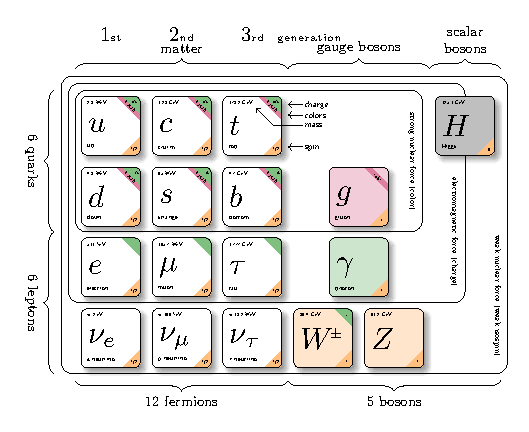
\includegraphics[width=0.8\textwidth]{figures/SM_figure.pdf}
\end{figure}
\section{The Standard Model}\label{ch:SM} %TODO: expand
In order to describe the three quantizable forces of nature, we gather the mediators of each force -- the vector bosons -- into local (gauge) symmetry groups. 
Each vector boson has one corresponding generator, the set of which constitutes the group.
The strong charge is mediated by eight massless gluons, which correspond to the eight independent generators of $\text{SU}(3)_C$. 
The weak charge is mediated by the three massive gauge bosons $W^\pm$ and $Z$, and the massless photon $\gamma$, 
which constitute the generators of $\text{SU}(2)_L$ and $\text{U}(1)_Y$. 

The subscript of each group denotes by which mechanism that force is mediated. The gluons mediate the strong force through interactions of color,
emphasized with subscript $C$. The weak force only sees left-handed particles, 
which we distinguish with the subscript $L$. And the electroweak interaction that a particle undergoes is determined by its hypercharge $Y$. 
For example, the quarks all have a non-zero color and non-zero hypercharge, 
so they participate in the strong and electromagnetic interactions. If a quark is left-handed, it will also feel the weak interaction. 
The neutrinos, on the other hand, have neither charge nor color, 
so they are invisible to both the strong and electromagnetic force. We express this by letting their fields transform as singlets under those symmetry groups.

\subsection{Beyond the Standard Model}
Together, these three interactions make up the Standard Model gauge group $\mathrm{SU}(3)_{\mathrm{C}} \times \mathrm{SU}(2)_{L} \times \mathrm{U}(1)_{Y}$. 
This determines the form of the three coupling constants, which numerical values must be experimentally measured. 
Since the vector bosons are represented by the generators, they are uniquely determined by the symmetry group. However, the scalar boson(s) and fermions are free as long as they
belong to representations of the symmetry group. By this construction, modifications to fermions rather than bosons are generally easier to make, allowing us to propose amendments to the model. Even the
number of fermions must be experimentally verified and can be altered from a phenomenological standpoint. In this work,
we will use this leniency to introduce a new particle and examine to which extent 
these modifications might be supported by experimental evidence. Moreover, we will examine the possibility of adding a new completely new force, which manifests itself as modifications to the neutrino-matter interactions.

\section{Mass Generation}
In the Standard Model, fermion masses are generated by the Higgs mechanism through Yukawa couplings with the fermion's right and left-handed components.
All neutrinos are left-handed and all antineutrinos are right-handed~\cite{giunti}. Thus, they do not pick up a Yukawa coupling, 
and will not undergo the Higgs mechanism, which leaves them massless.
Additionally, all terms of a Lagrangian that we construct must respect the gauge invariance. This removes the possibility of the neutrino mass to be 
generated at loop level because any such attempt will violate the total lepton number by two units.
In order to keep our theory renormalizable, we have one option left if we want to generate neutrino masses: introducing right-handed neutrinos and left-handed antineutrinos. 

We consider a right-handed neutrino field, $\nu_R$. Since the electroweak gauge group $\text{SU}(2)_L \times U(1)_Y$ only couple to 
left-handed particles and right-handed antiparticles, $\nu_R$ transforms as a singlet under the Standard Model symmetry 
group $\mathrm{SU}(3)_{\mathrm{C}} \times \mathrm{SU}(2)_{L} \times \mathrm{U}(1)_{Y}$. 

%TODO: write eq for lepton doublet

We extend the Standard Model by adding a right-handed component of this field with neutrino Yukawa couplings $Y_{\alpha \beta}^{\prime \nu}$ to the Higgs-lepton Yukawa part of the interaction Lagrangian 
\begin{align} % TODO: its not a Lorentz scalar, there has to be a bar somewhere. Is it incorrect?
    \mathcal{L}_{int} \subseteq -\left( \frac{v + H}{\sqrt{2}} \right) \left[\ell_{\alpha L}^{\prime} Y_{\alpha \beta}^{\prime \ell} \ell_{\beta R}^{\prime} + \nu_{\alpha L}^{\prime} Y_{\alpha \beta}^{\prime \nu} \nu_{\beta R}^{\prime}\right]\,,
\end{align}
where $v$ is the Higgs vacuum expectation value, $H$ the Higgs field, $\ell_{\alpha L}^\prime (\ell_{\beta R}^\prime)$ the left (right) handed charged lepton field. $Y_{\alpha \beta}^{\prime \ell}$ are the charged lepton Yukawa couplings, and $\nu^\prime_{\alpha L}(\nu^\prime_{\beta R})$ are the left (right) handed neutrino fields .
Now, the Yukawa coupling matrices $Y^{\prime \ell}$ and $Y^{\prime \nu}$ are non-diagonal. 
%TODO: Y  is not symmetric. We need to do a bi-unitary transformation. If you are not sure, just drop this.
%We need two diagonalizations here
This can be remedied by diagonalizing $Y^{\prime \nu}$ with a unitary matrix $V^\nu$ as
\begin{align}
    V_{\alpha k L}^{\nu \dagger} Y^{\prime \nu}_{\alpha \beta} V_{\beta j R}^{\nu}=Y^{\nu}_{kj} \,.
\end{align}
Similarly, we diagonalize and $Y^{\prime \nu}$ with a unitary matrix $V^\nu$. We note that this will not yet generate neutrino masses, 
since no flavor rotation can make massless fields massive.
Now we state a crucial difference between the properties of the charged lepton and the neutrino fields.
While the charged lepton flavor eigenstate was uniquely determined by its mass eigenstate, the neutrino flavor is a superposition of mass eigenstates. 
This is because neutrinos are indirectly detected via the observation of its associated charged lepton, so there is no requirement for neutrino flavor eigenstates to have a definite mass. 
The flavor of a neutrino is then, by definition, the flavor of the associated charged lepton. 
This fact is denoted as giving the mass eigenstates Latin numerals and letters, while the flavor eigenstates stay as Greek letters.

So, let the neutrino field in the mass basis have components with Latin numerals to distinguish them from the flavour components, i.e 
\begin{align}\label{eq:nu_rotation} 
    \nu_{k} =  V_{k\beta}^{\nu \dagger} \nu_{\beta}^\prime\,.
\end{align}
The diagonalized Lagrangian now takes the form 
\begin{align}
    \mathcal{L}_{int} &\subseteq -\left( \frac{v + H}{\sqrt{2}} \right) \left[\ell_{\alpha L}^{\prime} Y_{\alpha \beta}^{\prime \ell} \ell_{\beta R}^{\prime} + \nu_{\alpha L}^{\prime} Y_{\alpha \beta}^{\prime \nu} \nu_{\beta R}^{\prime}\right] \nonumber \\
    &= -\left( \frac{v + H}{\sqrt{2}} \right) \left[\ell_{\alpha L}^{\prime} V_{\alpha \beta L}^{\ell} Y_{\alpha \beta}^{ \ell} V_{\alpha \beta R}^{\ell \dagger} \ell_{\beta R}^{\prime}
    + \nu_{\alpha L}^{\prime} V_{\alpha k L}^{\nu} Y_{kj}^{\nu} V_{\beta j  R}^{\nu \dagger} \nu_{\beta R}^{\prime}\right] \nonumber \\
    &= -\left( \frac{v + H}{\sqrt{2}} \right) \left[\ell_{\alpha L}^\dagger Y_{\alpha \beta}^{ \ell} \ell_{\beta R} + \nu_{k L}^{\dagger} Y_{kj}^{ \nu} \nu_{j R}\right] \nonumber \\
    &= -\left( \frac{v + H}{\sqrt{2}} \right) \left[\bar{\ell}_{\alpha L} Y_{\alpha \beta}^{ \ell} \ell_{\beta R} + \bar{\nu}_{k L} Y_{kj}^\nu \nu_{j R}\right]
\end{align}
By construction, $Y^\ell$ and $Y^\nu$ are diagonal, so we write their components as $y_{\alpha}^{\ell} \delta_{\alpha \beta}$ and $y_{k}^{\nu} \delta_{k j}$ respectively, leaving the Lagrangian as 
\begin{align}\label{eq:L_H}
    \mathcal{L}_{int} 
    &\subseteq-\left( \frac{v + H}{\sqrt{2}} \right) \left[\bar{\ell}_{\alpha L} y_{\alpha}^{\ell} \delta_{\alpha \beta} \ell_{\beta R} + \bar{\nu}_{k L} y_{k}^{\nu} \delta_{k j} \nu_{j R}\right] \nonumber \\
    &=-\left( \frac{v + H}{\sqrt{2}} \right) \left[\bar{\ell}_{\alpha L} y_{\alpha}^{\ell}  \ell_{\alpha R} + \bar{\nu}_{k L} y_{k}^{\nu} \nu_{k R}\right] \nonumber \\
    &=-\left( \frac{v + H}{\sqrt{2}} \right) \left[ y_{\alpha}^{\ell}  \bar{\ell}_{\alpha L}\ell_{\alpha R} +  y_{k}^{\nu}\bar{\nu}_{k L} \nu_{k R}\right] 
\end{align}
Now, by the introduction of the right-handed field $\nu_R$, the Dirac neutrino field is
\begin{align}
    \nu_k = \nu_{kL} + \nu_{kR}\,.
\end{align}
Multiplying $\nu_k$ with its conjugate $\bar{\nu}_k$, we get 
\begin{align}
    \bar{\nu}_k \nu_k 
    & = \bar{\nu}_{k L} \nu_{k L} +\bar{\nu}_{k R}\nu_{k L} + \bar{\nu}_{k L}\nu_{k R} + \bar{\nu}_{k R}\nu_{k R} \nonumber \\
    & = \bar{\nu}_{k L}\nu_{k R} + \bar{\nu}_{k R}\nu_{k L} \nonumber \\
    & = \bar{\nu}_{k L}\nu_{k R} + \t{h.c.}
\end{align}
The same calculation for the charged lepton field yields the same result for $\ell_k$. Substituting this result and multiplying the Higgs vacuum expectation value $v$ into the fields gives us
\begin{align}
    \mathcal{L}_{H} 
    &=-\left( \frac{v + H}{\sqrt{2}} \right) \left[ y_{\alpha}^{\ell}   \bar{\ell}_\alpha \ell_\alpha  +  y_{k}^{\nu} \bar{\nu}_k \nu_k \right] \nonumber \\
    &=- \frac{y_{\alpha}^{\ell} v}{\sqrt{2}}   \bar{\ell}_\alpha \ell_\alpha   -  \frac{ y_{k}^{\nu} v}{\sqrt{2}} \bar{\nu}_k \nu_k  - \frac{y_{\alpha}^{\ell}}{\sqrt{2}}   \bar{\ell}_\alpha \ell_\alpha H  -  \frac{ y_{k}^{\nu}}{\sqrt{2}} \bar{\nu}_k \nu_k H\,.
\end{align}
Thus, this extension to the SM generates by the Higgs mechanism neutrino masses with terms
\begin{align}
    m_k = \frac{y_k^\nu v}{\sqrt{2}}\,,
\end{align}
where the Yukawa couplings $y^\nu_k$ needs to be experimentally determined.
% \documentclass[a4paper,10pt,draft]{thesis}
\usepackage{physics,amsmath, amsfonts, siunitx, amssymb, graphicx, slashed,subcaption}
\usepackage[utf8]{inputenc}
\usepackage[margin=1in]{geometry}
\usepackage[hidelinks]{hyperref}
\usepackage{xr-hyper}
\newcommand{\n}[1]{\nu_{#1}}
\newcommand{\na}{\nu_\alpha}
\newcommand{\nb}{\nu_\beta}
\newcommand{\ana}{\bar{\nu}_\alpha}
\newcommand{\an}[1]{\bar{\nu}_{\text{#1}}}
\newcommand{\anb}{\bar{\nu}_\beta}
\renewcommand{\a}{\alpha}
\renewcommand{\b}{\beta}
\newcommand{\ab}{\alpha\beta}


\renewcommand{\ne}{\nu_e}
\newcommand{\nm}{\nu_\mu}
\newcommand{\nt}{\nu_\tau}
\newcommand{\ns}{\nu_s}

\newcommand{\ane}{\bar{\nu}_e}
\newcommand{\anm}{\bar{\nu}_\mu}
\newcommand{\ant}{\bar{\nu}_\tau}
\newcommand{\ans}{\bar{\nu}_s}

\newcommand{\nee}{\nu_e \to \nu_e}
\newcommand{\nem}{\nu_e \to \nu_\mu}
\newcommand{\net}{\nu_e \to \nu_\tau}
\newcommand{\nes}{\nu_e \to \nu_s}

\newcommand{\nme}{\nu_\mu \to \nu_e}
\newcommand{\nmm}{\nu_\mu \to \nu_\mu}
\newcommand{\nmt}{\nu_\mu \to \nu_\tau}
\newcommand{\nms}{\nu_\mu \to \nu_s}



\newcommand{\Pee}{P_{e  e}}
\newcommand{\Pem}{P_{e  \mu}}
\newcommand{\Pet}{P_{e  \tau}}
\newcommand{\Pes}{P_{e  s}}

\newcommand{\Pme}{P_{\mu  e}}
\newcommand{\Pmm}{P_{\mu\mu}}
\newcommand{\Pmt}{P_{\mu  \tau}}
\newcommand{\Pms}{P_{\mu  s}}


\newcommand{\Pte}{P_{P_{\tau e}}}
\newcommand{\Ptm}{P_{\tau  \mu}}
\newcommand{\Ptt}{P_{\tau  \tau}}
\newcommand{\Pts}{P_{\mu  s}}

\newcommand{\Paeae}{P_{\bar{e}  \bar{e}}}
\newcommand{\Paeam}{P_{\bar{e}  \bar{\mu}}}
\newcommand{\Paeat}{P_{\bar{e}  \bar{\tau}}}
\newcommand{\Paeas}{P_{\bar{e}  \bar{s}}}

\newcommand{\Pamae}{P_{\bar{\mu}  \bar{e}}}
\newcommand{\Pamam}{P_{\bar{\mu}  \bar{\mu}}}
\newcommand{\Pamat}{P_{\bar{\mu}  \bar{\tau}}}
\newcommand{\Pamas}{P_{\bar{\mu}  \bar{s}}}


\newcommand{\Patae}{P_{\bar{\tau}  \bar{e}}}
\newcommand{\Patam}{P_{\bar{\tau}  \bar{\mu}}}
\newcommand{\Patat}{P_{\bar{\tau}  \bar{\tau}}}
\newcommand{\Patas}{P_{\bar{\mu}  \bar{s}}}

\renewcommand{\th}[1][]{%
  \theta\ifx\\#1\\\else_\text{#1}\fi
}
\newcommand{\thm}[1][]{%
  \theta^\text{M}\ifx\\#1\\\else_\text{#1}\fi
}
\renewcommand{\t}[1]{\text{{#1}}}
\newcommand{\avg}[1]{\left\langle {#1} \right \rangle}
\newcommand*{\dm}[1][]{%
  \Delta m^2\ifx\\#1\\\else_\text{#1}\fi
}
\newcommand{\zreco}{\cos{(\theta_z^{reco})}}
\newcommand{\ztrue}{\cos{(\theta_z^{true})}}
\newcommand{\z}{\cos{(\theta_z)}}
\newcommand{\Ereco}{E^{reco}}
\newcommand{\Etrue}{E^{true}}
\newcommand{\Aeff}{A^\text{eff}}
\newcommand{\emm}{\epsilon_{\mu\mu}}
\newcommand{\emt}{\epsilon_{\mu\tau}}
\newcommand{\eet}{\epsilon_{e\tau}}
\newcommand{\eem}{\epsilon_{e\mu}}
\newcommand{\ett}{\epsilon_{\tau\tau}}
\newcommand{\ep}{\epsilon^\prime}

% \begin{document}

\section{Neutrino Mixing}\label{ch:oscillation}
In 1998, the Super-Kamiokande collaboration detected a $\nm$ deficit that could not be explained by any other mechanism
than the conversion muon neutrinos to electron neutrinos. This was the first conclusive evidence of a $\nm \to \ne$ oscillation.
The most interesting conclusion from the observation of neutrino flavor oscillations is the equivalence between oscillations and neutrino mass, 
with the latter being identically zero acording to the Standard Model. Thus, we are required to extend the Standard Model to incorporate neutrino 
masses and hence, neutrino oscillations.

\subsection{Mass Generation}
In the Standard Model, fermion masses are generated by the Higgs mechanism through Yukawa couplings with the fermions right and left-handed components.
All neutrinos are left-handed and all antineutrinos are right-handed. Thus, neutrinos are massless since they do not undergo the Higgs mechanism.
Additionally, all terms of a Lagrangian that we construct must respect the gauge invariance. This removes the possibility of the neutrino mass to be 
generated at loop level because any such attempt will violate the total lepton number by two units.
In order to keep our theory renormalizable, we have one option left if we want to generate neutrino masses: introducing additional fermions. 

We consider a right-handed neutrino field, $\nu_R$. Since the electroweak gauge group $\text{SU}(2)_L \times U(1)_Y$ only couple to 
left-handed particles and right-handed antiparticles, $\nu_R$ transforms as a singlet under the Standard Model symmetry 
group $\mathrm{SU}(3)_{\mathrm{C}} \times \mathrm{SU}(2)_{L} \times \mathrm{U}(1)_{Y}$. 
This neutrino field is \emph{sterile} since it doesn't participate any of the Standard Model interactions. 

We extend the Standard Model by adding a right-handed component of this field with neutrino Yukawa couplings $Y_{\alpha \beta}^{\prime \nu}$ to the Higgs-lepton Yukawa Lagrangian 
\begin{align}
    \mathcal{L}_{H}=-\left( \frac{v + H}{\sqrt{2}} \right) \left[\ell_{\alpha L}^{\prime} Y_{\alpha \beta}^{\prime \ell} \ell_{\beta R}^{\prime} + \nu_{\alpha L}^{\prime} Y_{\alpha \beta}^{\prime \nu} \nu_{\beta R}^{\prime}\right]\,.
\end{align}
Now, the Yukawa coupling matrices $Y^{\prime \ell}$ and $Y^{\prime \nu}$ are non-diagonal, with the former resulting in the charged lepton masses being non-definite. 
This can be remedied by diagonalizing $Y^{\prime \ell}$ with a unitary matrix $V^\ell$ as
\begin{align}
    V_{\alpha k L}^{\nu \dagger} Y^{\prime \nu}_{\alpha \beta} V_{\beta j R}^{\nu}=Y^{\nu}_{kj} \,.
\end{align}
Similarily, we diagonalize and $Y^{\prime \nu}$ with a unitary matrix $V^\nu$. We note that this will not yet generate neutrino masses, since no flavor rotation can make massless fields massive.
Now we state a crucial difference between the properties of the charged lepton and the neutrino fields.
While the charged lepton flavor eigenstate was uniquely determined by its mass eigenstate, the neutrino flavor is a superposition of mass eigenstates. 
This is because neutrinos are indirectly detected via the observation of its associated charged lepton, so there is no requirement of neutrino flavor eigenstates to have a definite mass. 
The flavor of a neutrino is then, by definition, the flavor of the associated charged lepton. 
This fact is introduced as giving the mass eigenstates Latin numerals and letters, while the flavor eigenstates stay as Greek letters.

So, let the neutrino field with chriality $X$ be denoted $\nu_X$, with components having Latin numerals to distinguish them from the flavour components, i.e 
\begin{align}\label{eq:nu_rotation}
    \nu_{k X} =  V_{k\beta X}^{\nu \dagger} \nu_{\beta X}^\prime\,.
\end{align}
The diagonalized Lagrangian now takes the form 
\begin{align}
    \mathcal{L}_{H} &= -\left( \frac{v + H}{\sqrt{2}} \right) \left[\ell_{\alpha L}^{\prime} Y_{\alpha \beta}^{\prime \ell} \ell_{\beta R}^{\prime} + \nu_{\alpha L}^{\prime} Y_{\alpha \beta}^{\prime \nu} \nu_{\beta R}^{\prime}\right] \nonumber \\
    &= -\left( \frac{v + H}{\sqrt{2}} \right) \left[\ell_{\alpha L}^{\prime} V_{\alpha \beta L}^{\ell} Y_{\alpha \beta}^{ \ell} V_{\alpha \beta R}^{\ell \dagger} \ell_{\beta R}^{\prime}
    + \nu_{\alpha L}^{\prime} V_{\alpha k L}^{\nu} Y_{kj}^{\nu} V_{\beta j  R}^{\nu \dagger} \nu_{\beta R}^{\prime}\right] \nonumber \\
    &= -\left( \frac{v + H}{\sqrt{2}} \right) \left[\ell_{\alpha L}^\dagger Y_{\alpha \beta}^{ \ell} \ell_{\beta R} + \nu_{k L}^{\dagger} Y_{kj}^{ \nu} \nu_{j R}\right] \nonumber \\
    &= -\left( \frac{v + H}{\sqrt{2}} \right) \left[\bar{\ell}_{\alpha L} Y_{\alpha \beta}^{ \ell} \ell_{\beta R} + \bar{\nu}_{k L} Y_{kj}^\nu \nu_{j R}\right]
\end{align}
By construction, $Y^\ell$ and $Y^\nu$ are diagonal, so we write their omponents as $y_{\alpha}^{\ell} \delta_{\alpha \beta}$ and $y_{k}^{\nu} \delta_{k j}$ respectively, leaving the Lagrangian as 
\begin{align}\label{eq:L_H}
    \mathcal{L}_{H} 
    &=-\left( \frac{v + H}{\sqrt{2}} \right) \left[\bar{\ell}_{\alpha L} y_{\alpha}^{\ell} \delta_{\alpha \beta} \ell_{\beta R} + \bar{\nu}_{k L} y_{k}^{\nu} \delta_{k j} \nu_{j R}\right] \nonumber \\
    &=-\left( \frac{v + H}{\sqrt{2}} \right) \left[\bar{\ell}_{\alpha L} y_{\alpha}^{\ell}  \ell_{\alpha R} + \bar{\nu}_{k L} y_{k}^{\nu} \nu_{k R}\right] \nonumber \\
    &=-\left( \frac{v + H}{\sqrt{2}} \right) \left[ y_{\alpha}^{\ell}  \bar{\ell}_{\alpha L}\ell_{\alpha R} +  y_{k}^{\nu}\bar{\nu}_{k L} \nu_{k R}\right] 
\end{align}
Now, by the introduction of the sterile field $\nu_R$, the Dirac neutrino field is
\begin{align}
    \nu_k = \nu_{kL} + \nu_{kR}\,.
\end{align}
Multiplying $\nu_k$ with its conjugate $\bar{\nu}_k$, we get 
\begin{align}
    \bar{\nu}_k \nu_k 
    & = \bar{\nu}_{k L} \nu_{k L} +\bar{\nu}_{k R}\nu_{k L} + \bar{\nu}_{k L}\nu_{k R} + \bar{\nu}_{k R}\nu_{k R} \nonumber \\
    & = \bar{\nu}_{k L}\nu_{k R} + \bar{\nu}_{k R}\nu_{k L} \nonumber \\
    & = \bar{\nu}_{k L}\nu_{k R} + \t{h.c.}
\end{align}
The same calculation for the charged lepton field yields the same result for $\ell_k$. Substituting this result and expanding the Higgs vacuum expectation value $v$ into the fields gives us
\begin{align}
    \mathcal{L}_{H} 
    &=-\left( \frac{v + H}{\sqrt{2}} \right) \left[ y_{\alpha}^{\ell}   \bar{\ell}_\alpha \ell_\alpha  +  y_{k}^{\nu} \bar{\nu}_k \nu_k \right] \nonumber \\
    &=- \frac{y_{\alpha}^{\ell} v}{\sqrt{2}}   \bar{\ell}_\alpha \ell_\alpha   -  \frac{ y_{k}^{\nu} v}{\sqrt{2}} \bar{\nu}_k \nu_k  - \frac{y_{\alpha}^{\ell}}{\sqrt{2}}   \bar{\ell}_\alpha \ell_\alpha H  -  \frac{ y_{k}^{\nu}}{\sqrt{2}} \bar{\nu}_k \nu_k H\,.
\end{align}
Thus, this extension to the SM generates by the Higgs mechanism neutrino masses with terms
\begin{align}
    m_k = \frac{y_k^\nu v}{\sqrt{2}}\,,
\end{align}
where the Yukawa couplings $y^\nu_k$ needs to be experimentally determined.
\subsection{The Mixing Matrix}
Substituting the new transformation from Eq.~\ref{eq:nu_rotation} into the expression for the weak charged current, we get
\begin{align}\label{eq:j_CC2}
    j^\rho_L &= 2\bar{\nu}^\prime_{\alpha L} \gamma^\rho \ell_{\alpha L}^\prime \nonumber \\
             &= 2\bar{\nu}_{k L} V^{\prime \nu \dagger}_{k \alpha}V^{\prime \ell}_{\alpha \alpha} \gamma^\rho  \ell_{\alpha L}
\end{align}
Now, the current in Eq.~\ref{eq:j_CC2} conserves lepton number, since the neutrino field with flavor $\alpha$ only couples to the lepton field with flavor $\alpha$. 
Thus, neutrino interactions still conserve lepton number.
However, the Higgs-lepton Yukawa Lagrangian 
in Eq.~\ref{eq:L_H} violates lepton number conservation since it couples the charged lepton flavor $\alpha$ to the neutrino mass eigenstate $k$, which is a superposition of flavors. 
There is no transformation that leaves both the interaction and kinetic Lagrangian invariant, thus violating this symmetry.


Call $V^{\prime \nu \dagger}_{k \alpha}V^{\prime \ell}_{\alpha \alpha} = U^\dagger_{k \alpha}$. We will refer to the matrix $U$ built by the components $U_{k \alpha}$ as the
Pontecorvo-Maki-Nakagawa-Sakata (PMNS) matrix~\cite{pontecorvo1957,maki1962}. %TODO: source
We now have 
\begin{align}\label{eq:j_CC3} %TODO: put sums on all above?
    j^\rho_L &= 2 \sum_\alpha \sum_k U^\dagger_{\alpha k} \bar{\nu}_{k L} \gamma^\rho  \ell_{\alpha L}\,.
\end{align}

What form does this new matrix $U$ take? By construction, it provides the unitary transformation between the flavor and mass bases.
Any unitary $3\times3$ matrix can be parametrized using three mixing angles and six phases. However, not all phases affect the 
charged and weak currents and are thus not observable. Moreover, both the Lagrangian and the currents are invariant under global $U(1)$ transformations,
leaving only one physical phase for us to measure. Thus we are down to four degrees of freedom in the three dimensional case: three mixing angles
of the form $\sin{(\theta_{ij})}/\cos{(\theta_{ij})} = s_{ij}/c_{ij}$, and one phase of the form $e^{i\delta}$.

We construct the PMNS matrix using the rotation matrixes from $SO(3)$ as
\begin{align}
    U &= R_{23}R_{13,\delta_{\text{CP}}}R_{12} \nonumber \\
      & = 
    \begin{pmatrix}1 & 0 & 0 \\ 0 & c_{23} & s_{23} \\ 0 & -s_{23} & c_{23}\end{pmatrix}
\begin{pmatrix}c_{13} & 0 & s_{13} e^{-i \delta_{\mathrm{CP}}} \\ 0 & 1 & 0 \\ -s_{13} e^{i \delta_{\mathrm{CP}}} & 0 & c_{13}\end{pmatrix}
\begin{pmatrix}c_{12} & s_{12} & 0 \\ -s_{12} & c_{12} & 0 \\ 0 & 0 & 1\end{pmatrix}\,.
\end{align}
The term $\delta_\text{CP}$ determines the degree of charge-parity violation. In this work, we will assume CP invariance by always
setting $\delta_{CP} = \SI{0}{\degree}$. Thus,

\begin{align}
    U &=
    \begin{pmatrix}1 & 0 & 0 \\ 0 & c_{23} & s_{23} \\ 0 & -s_{23} & c_{23}\end{pmatrix}
\begin{pmatrix}c_{13} & 0 & s_{13} \\ 0 & 1 & 0 \\ -s_{13}  & 0 & c_{13}\end{pmatrix}
\begin{pmatrix}c_{12} & s_{12} & 0 \\ -s_{12} & c_{12} & 0 \\ 0 & 0 & 1\end{pmatrix} \nonumber \\
    &= 
    \begin{pmatrix}c_{12} c_{13} & s_{12} c_{13} & s_{13} \\ 
        -s_{12} c_{23}-c_{12} s_{23} s_{13} & c_{12} c_{23}-s_{12} s_{23} s_{13} & s_{23} c_{13} \\ 
        s_{12} s_{23}-c_{12} c_{23} s_{13}  & -c_{12} s_{23}-s_{12} c_{23} s_{13} & c_{23} c_{13}
    \end{pmatrix}\,.
\end{align}

In this work, we will be using the best-fit values from~\cite{nufit} with the exception of the CP-violating phase $\delta_\text{CP}$. The $90\% $ CL values are
\begin{align}\label{eq:nufitparams}
    \theta_{12} = \SI{33.44}{\degree},\hspace{1em} \theta_{13} = \SI{8.57}{\degree},\hspace{1em} \theta_{23} = \SI{49.2}{\degree}, \hspace{1em} \delta_\text{CP} = 0\,.
\end{align}
The PMNS matrix is then real, with numerical values 
\begin{align}\label{eq:Uvalues}
    U = \begin{pmatrix}
        U_{e 1} & U_{e2} & U_{e3} \\
        U_{\mu 1} & U_{\mu 2} & U_{\mu 3} \\
        U_{\tau 1} & U_{\tau 2} & U_{\tau 3}
    \end{pmatrix} 
    = \begin{pmatrix}
        0.825 & 0.545 & 0.149 \\
        -0.455 & 0.485 & 0.746 \\
        0.334 & -0.684 & 0.649
    \end{pmatrix} \,.
\end{align}
In our study, we will only use neutrinos originating from conventional cosmic ray interactions in the atmosphere. 
In this so-called atmospheric neutrino flux, $\nm$ are the most abundant, while the $\nt$ flux is neglible. We see that $U_{\mu\tau}$ is the largest $U_{\mu\beta}$ term,
suggesting that $\nm$ primarily mixes into $\nt$, at least in vacuum. It turns out that matter effects indeed preserves this ordering, making the $\nm \to \nt$ transition
the most abundant. This means we will be able to stringently constrain parameters relating to $\mu\tau$ mixing.

\subsection{Neutrino Propagation}
Since we now know how the neutrino mass and flavor eigenstates combine, and have an expression for the flavor interaction with 
the neutrino's charged lepton partner, we are now ready to study the flavor oscillations themselves.

Now, the Fourier expansion of the field operator $\bar{\nu}_{k L}$ in the current of Eq.~\ref{eq:j_CC3} contains creation operators $a^\dagger_{\nu_k}$
of massive neutrinos with mass $m_k$. This means that the summation over the mass index $k$ constructs a flavor neutrino, which interacts with the charged lepton field $\ell_{\a L}$.
In other words, the charged current generates a flavor neutrino $\na$, which is a superposition of the mass eigenstates 
$\nu_k$ with weights $U_{\a k}^\dagger$. In the ket-formalism, we express this as
\begin{align}\label{eq:osc_1}
    \ket{\na} = \sum_k U^\dagger_{\a k} \ket{\nu_k}\,.
\end{align}
It is the mass eigenstates $\ket{\nu_k}$ that are eigenstates of the Hamiltonian, with eigenvalues
\begin{align}\label{eq:disp}
    E_k = \sqrt{\vec{p}^2 + m_k^2}\,.
\end{align}
The solution to the time-dependent Schrödinger equation 
\begin{align}\label{eq:TDSE}
    i \dv{}{t} \ket{\nu_k(t)} = H_0\ket{\nu_k(t)}\,,
\end{align}
where $H_0$ is the Hamiltonian and the subscript signifies that we are in vacuum. 

The solution to Eq.~\ref{eq:TDSE} gives ut the time evolution
in the form of plane wave solutions: 
\begin{align}
    \ket{\nu_k(t)} = e^{-iE_kt}\ket{\nu_k}\,.
\end{align}
Inserting the plane wave solution into Eq.~\ref{eq:osc_1}, we get 
\begin{align}\label{eq:nat}
    \ket{\na(t)} = \sum_k U^\dagger_{\a k} e^{-iE_kt}\ket{\nu_k}\,.
\end{align}
Now we know how to evolve and combine the mass eigenstates to form a flavor eigenstate, but how about the reverse?
 We swap the index $k\to j$ in Eq.~\ref{eq:osc_1} and multiply by $U_{\a k}$:
\begin{align}\label{eq:osc_k}
    \sum_\a U_{\a k}\ket{\na} &= \sum_{\alpha, j} U_{\a k} U_{\a j}^\dagger \ket{\nu_j} \nonumber \\
    \sum_\a U_{\a k}\ket{\na} &= \sum_{j} \delta_{kj} \ket{\nu_j} \nonumber \\
    \sum_\a U_{\a k}\ket{\na} &= \ket{\nu_k}\,,
\end{align}
where we have used the unitarity of the leptonic mixing matrix. Eqs.~\ref{eq:osc_1} and \ref{eq:nat} yield 
\begin{align}
    \ket{\na(t)} &= \sum_k U^\dagger_{\a k} e^{-iE_kt}\ket{\nu_k} \nonumber \\
    \ket{\na(t)} &= \sum_k U^\dagger_{\a k} e^{-iE_kt}\left(\sum_\b U_{\b k}\ket{\nb}\right) \nonumber \\
    \ket{\na(t)} &= \sum_{k,\b} U^\dagger_{\a k}U_{\b k} e^{-iE_kt} \ket{\nb}\,.
\end{align}
The probability of the flavor transition $\na \to \nb$ at time $t$ is $\abs{\bra{\nb}\ket{\na (t)}}^2$:
\begin{align}
    P_{\na \to \nb}(t) = \sum_{k,j} U^\dagger_{\a k}U_{\b k}U^*_{\b j}U_{\a j} e^{-i(E_k-E_j)t}\,.
\end{align}

We assume the neutrino masses $m_k$ to be extremely small compared to their associated energies $E_k$. 
Thus, $v\sim 1$, and $\abs{\vec{p}} \sim E$ making the energy-dispersion relation of Eq.~\ref{eq:disp} to first order:
\begin{align}\label{eq:ultra_rel}
    E_k &= \sqrt{\vec{p}^2 + m_k^2} \nonumber \\
        &= \vec{p}^2\sqrt{1 + \frac{m_k^2}{\vec{p}^2}} \nonumber \\
        &\approx E + \frac{m_k^2}{2E}
\end{align}
Hence, the exponential can be simplified, and simplifying the notation $P_{\na \to \nb}(t) \to P_{\ab}(t)$ we get 
\begin{align}
    P_{\ab}(t) = \sum_{k,j} U^\dagger_{\a k}U_{\b k}U^\dagger_{\b j}U_{\a j} e^{-i(m_k^2-m_j^2)t/2E}\,.
\end{align}
Now, our approximation $v\approx 1$ implies $x\approx t $, thus
\begin{align}
    P_{\ab}(x) &= \sum_{k,j} U^\dagger_{\a k}U_{\b k}U^\dagger_{\b j}U_{\a j} e^{-i(m_k^2-m_j^2)x/2E} \nonumber \\
                       &= \sum_{k,j} U^\dagger_{\a k}U_{\b k}U^\dagger_{\b j}U_{\a j} \exp(-i\frac{\dm_{kj}x}{2E})\,,
\end{align}
where we in the last step have defined the \emph{mass squared-difference} $\dm_{kj} = m_k^2 - m_j^2$. Since the oscillation probability depends on this quantity
rather than the individual masses, it is impossible
to measure the mass $m_k$ through neutrino oscillations.
Squaring the unitarity condition $\sum_k U_{\a k}U_{\b k}^\dagger = \delta_{\a \b}$ yields 
\begin{align}
    \sum_k \abs{U_{\a k}}^2\abs{U_{\b k}}^2 = \delta_{\a \b} - 2 \sum_{k>j}\Re[U_{\a k}^\dagger U_{\b k} U_{\a j} U_{\b j}^\dagger]
\end{align}
Since we take the PMNS matrix to be real and thus Hermitian, we drop the complex transpose in the following calculation. We have
\begin{align}\label{eq:Pab}%TODO: shorten?
    P_{\ab} &= \sum_{k,j} U_{\a k}U_{\b k}U_{\b j}U_{\a j} \exp(-i\frac{\dm_{kj}x}{2E}) \nonumber \\
            &=  \sum_k \abs{U_{\a k}}^2\abs{U_{\b k}}^2 + \sum_{k \neq j} U_{\a k}U_{\b k}U_{\b j}U_{\a j} \exp(-i\frac{\dm_{kj}x}{2E}) \nonumber \\
            &= \delta_{\a \b} - 2 \sum_{k>j}U_{\a k} U_{\b k} U_{\b j} U_{\a j} +\sum_{k \neq j} U_{\a k}U_{\b k}U_{\b j}U_{\a j} \exp(-i\frac{\dm_{kj}x}{2E}) \nonumber \\
            &= \delta_{\a \b} - 2 \sum_{k>j}U_{\a k} U_{\b k} U_{\b j} U_{\a j} + 2\sum_{k > j} U_{\a k}U_{\b k}U_{\b j}U_{\a j} \exp(-i\frac{\dm_{kj}x}{2E}) \nonumber \\
            &= \delta_{\a \b} - 2\sum_{k > j} U_{\a k}U_{\b k}U_{\b j}U_{\a j} \left[1-\exp(-i\frac{\dm_{kj}x}{2E})\right] \nonumber \\
            &= \delta_{\a \b} - 2\sum_{k > j} U_{\a k}U_{\b k}U_{\b j}U_{\a j} \left[1-\cos(\frac{\dm_{kj}x}{2E})\right] \nonumber \\
            &= \delta_{\a \b} - 2\sum_{k > j} U_{\a k}U_{\b k}U_{\b j}U_{\a j} \sin^2{\left(\frac{\dm_{kj}x}{4E}\right)}\,,
\end{align}
which is the probability of neutrino vacuum oscillations. %TODO: maybe plot?
The calculation for antineutrinos yield the same result if one continues to assume the realness of the mixing matrix. 
In Fig.~\ref{fig:vac_osc}, we show the energy spectra of these oscillations in the low \si{\GeV} range for neutrinos that travel \SI{12000}{\km}\footnote{This baseline
is approximately the Earth diameter, and will be the maximum travel distance which we will use later on.}.
In the left-most panel, we see a supressed $\nu_\mu \to e$ transition. We can understand this behavior by studying Eq.~\ref{eq:Pab} and the 
numerical values of the mixing matrix in Eq.~\ref{eq:Uvalues}.
\si{\GeV} oscillations are driven by the $\dm[31]$ mass-squared difference. Hence, the most important mixing matrix 
elements for $P_{\a\b}$ are $U_{\a3}, U_{\a1}$ and $U_{\b3}, U_{\b1}$. The smallness of $U_{e3}$ then supresses the
amplitude of $\Pme$.
\begin{figure}
    \centering
    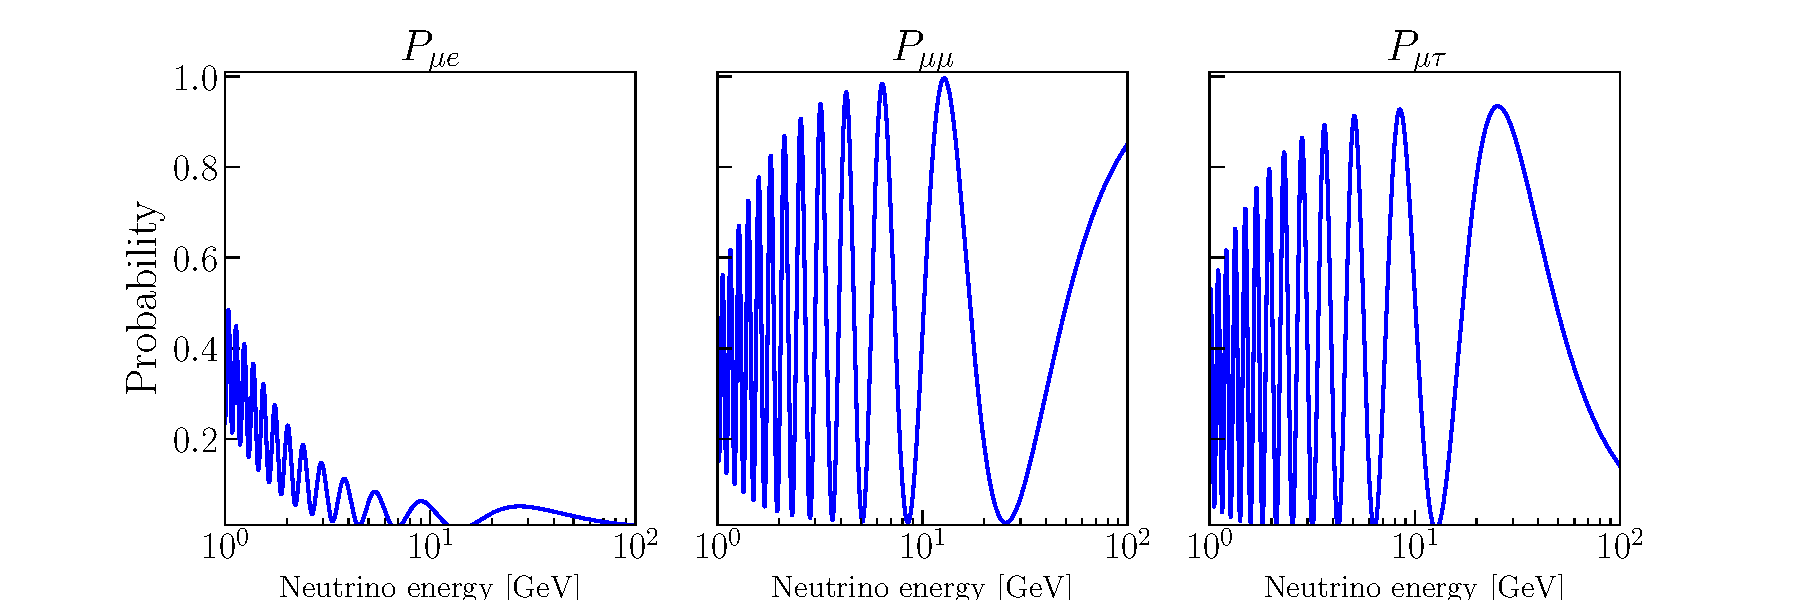
\includegraphics[width=0.9\textwidth]{figures/vac_osc.pdf}
    \caption{$\nm$ vacuum oscillations from Eq.~\ref{eq:Pab}}\label{fig:vac_osc}
\end{figure}

For our purposes, the probabilities in Eq.~\ref{eq:Pab} are rather uninteresting, since they are only valid in vacuum.
Despite this fact, this form elucidates an important aspect of neutrino oscillations. The mixing matrix elements
determine the amplitude of the oscillations, while the mass-squared differences together with the ratio $L/E$ determine the 
frequency. 

\subsection{Effective Potentials}

\begin{figure}
    \centering
    \begin{subfigure}{0.3\textwidth}
        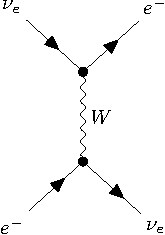
\includegraphics[width=0.9\textwidth]{figures/w-boson.pdf} 
        \caption{Charged current weak interaction between an electron neutrino and an electron,
        mediated by either a $W^+$ or $W^-$ boson.}
    \end{subfigure}
    \quad
    \begin{subfigure}{0.3\textwidth}
        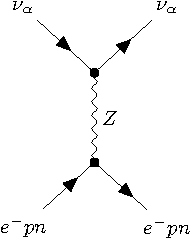
\includegraphics[width=1\textwidth]{figures/z-boson.pdf} 
        \caption{Neutral current weak interaction between a neutrino of any flavor and a Earth-like fermion,
        mediated by a neutral $Z$ boson.}
    \end{subfigure}%TODO: they are different sizes
    \caption{Feyman diagrams showing the two interactions that neutrinos participate in according to the Standard Model.}\label{fig:w_and_z}
\end{figure}
In this work, we are concerned about the interactions with the neutrino and Earth-like matter, i.e.~electrons, protons, and neutrons. 
The possible interactions are shown in Fig.~\ref{fig:w_and_z}. The left panel shows that the only flavor that can go through charged current (CC) 
interactions is the electron flavor. This is because the Earth doesn't consist of any muons or tau particles. 
The right panel shows any neutrino flavor interaction via the neutral current (NC) with Earth-like matter\footnote{The Earth is entirely composed
of electrons, protons, and neutrons. Thus, the fundamental particles composing Earth are electrons, and up and down quarks. We refer to this as \emph{Earth-like matter}.}, mediated by the neutral $Z$ boson
The interaction mediated by the $W$ boson will give rise to a effective matter potential $V_{CC}$, while
the $Z$ boson is responsible for $V_{NC}$. Our task is now to find expressions for these.

We start with the effective Hamiltonian for the CC process. The Feynman rules for the left panel give us 
\begin{align}
    H_{CC} = \frac{G_F}{\sqrt{2}}\left[ \bar\ne \gamma^\rho\, (1- \gamma^5)\, e \right] \left[\bar e \,\gamma_\rho\, (1- \gamma^5)\, \ne \right]
\end{align}
By using the Fierz transformation 
\begin{align}
    \mathcal{L}^{V-A}(\psi_1,\psi_2,\psi_3,\psi_4) = \mathcal{L}^{V-A}(\psi_1,\psi_4,\psi_3,\psi_2)\,,
\end{align}
we can permute the terms inside the brackets, yielding
\begin{align}\label{eq:H_fierz}
    H_{CC} = \frac{G_F}{\sqrt{2}}\left[ \bar\ne \gamma^\rho\, (1- \gamma^5)\, \ne \right] \left[\bar e \,\gamma_\rho\, (1- \gamma^5)\, e \right]\,.
\end{align}
Now, lets consider a finite volume $V$ with electron states defined as 
\begin{align}\label{eq:e_states}
    \ket{e(p_e,h_e)} = \frac{1}{2E_eV}a_e^{(h_e)\dagger}(p_e)\ket{0}\,,
\end{align}
i.e. using the creation operator $a_e^{(h_e)\dagger}(p_e)$ to create electron states from vacuum with momenta $p_e$, energy $E_e$, and helicity $h_e$.
The density distribution of electrons in $V$ is $f(E_e,T)$, which we normalize to the total number of electrons as we integrate out the momenta $p_e$:
\begin{align}\label{eq:e_density}
    \int \dd p_e^3 f(E_e,T) = N_e V = n_e
\end{align}
Here, the electron density $N_e$ will ultimately determine the strength of the effective matter potential. 
To obtain the average effective Hamiltonian, project it on the electron states in Eq.~\ref{eq:e_states} and integrate over the density and sum over the helicities:

\begin{align}\label{eq:avg_H1}
    \avg{H_{CC}} &= \int \dd p_e^3 \bra{e(p_e,h_e)} \times \frac{1}{2} \sum_{h_e} H   f(E_e,T) \ket{e(p_e,h_e)} \nonumber \\
           &= \frac{G_F}{\sqrt{2}} \int \dd p_e^3 \bra{e(p_e,h_e)} \left[ \bar\ne \gamma^\rho\, (1- \gamma^5)\, \ne \right]  f(E_e,T) \times \frac{1}{2} \sum_{h_e} \left[\bar e(x) \,\gamma_\rho\, (1- \gamma^5)\, e(x) \right] \ket{e(p_e,h_e)} \nonumber \\
           &= \frac{G_F}{\sqrt{2}} \bar\ne \gamma^\rho\, (1- \gamma^5)\, \ne \int \dd p_e^3  f(E_e,T) \times \frac{1}{2} \sum_{h_e} \bra{e(p_e,h_e)} \bar e(x) \,\gamma_\rho\, (1- \gamma^5)\, e(x)   \ket{e(p_e,h_e)}\,.
\end{align}
First, calculate the sum using trace technology %TODO: explain this more
\begin{align}\label{eq:helicity_sum}
    \frac{1}{2} \sum_{h_e} \bra{e(p_e,h_e)} \bar e(x) \,\gamma_\rho\, (1- \gamma^5)\, e(x)   \ket{e(p_e,h_e)} &= \frac{1}{4E_e V} \sum_{h_e} \bar{u}_e^{h_e}(p_e) \,\gamma_\rho\, (1- \gamma^5)\, u_e^{h_e}(p_e) \nonumber \\
    &= \frac{1}{4 E_e V} \Trace{\left[ \sum_{h_e} \bar{u}_e^{h_e}(p_e) u_e^{h_e}(p_e) \,\gamma_\rho\, (1- \gamma^5)\, \right]} \nonumber \\
    &= \frac{1}{4 E_e V} \Trace{\left[ (\slashed{p}_e + m_e ) \,\gamma_\rho\, (1- \gamma^5)\, \right]} \nonumber \\
    &= \frac{(p_e)_\rho}{E_e V}\,.
\end{align}
Eq.~\ref{eq:avg_H1} now becomes 
\begin{align}\label{eq:avg_H2}
    \avg{H_{CC}} &= \frac{G_F}{\sqrt{2}E_e V} \bar\ne \, (1- \gamma^5)\, \ne \int \dd p_e^3\, \slashed{p}_e\, f(E_e,T)\,.
\end{align}
Expand the integral, and use the fact that $\vec{p}_e$ is odd:
\begin{align}
    \int \dd p_e^3\, \slashed{p}_e\, f(E_e,T) &= \int \dd p_e^3\, f(E_e,T) (\gamma^0 E_e - \vec{p}_e \cdot \vec{\gamma}) \nonumber \\
                                              &= \int \dd p_e^3\, f(E_e,T) \gamma^0 E_e \nonumber \\
                                              &= \gamma_0 E_e N_e V\,.
\end{align}
Inserting this into Eq.~\ref{eq:avg_H2}, we have
\begin{align}
    \avg{H_{CC}} &= \frac{G_F N_e}{\sqrt{2}} \bar{\nu}_e \, (1- \gamma^5)\, \ne \gamma_0 \nonumber \\
            &= \sqrt{2}G_F N_e \bar{\nu}_{eE} \gamma^0 \nu_{eL}\,,
\end{align}
where the projection operator $(1- \gamma^5)$ in the first line ensures that only the left-hand compontent of the neutrino fields interact. Thus,
\begin{align}\label{eq:V_CC1}
    V_{CC} = \sqrt{2}G_F N_e\,, \quad H_{CC}\ket{\nu_k} = V_{CC}\ket{\nu_k}\,.
\end{align}
Here we see a crucial difference between the eigenvectors between the vacuum Hamiltonian defined in Eq.~\ref{eq:osc_1} and $H_{CC}$, namely
that the CC interactions happen in the flavor basis rather than in the mass basis\footnote{A similar calculation for the NC reveals the same fact:
neutrinos interact in the flavor basis.}. In other words,
neutrinos propagate in their mass eigenstates, but interact in their flavor eigenstate. The mixing of mass eigenstates during propagation
determines if the flavor eigenstate has oscillated or not. The interactions still conserve lepton number, but the kinetic Lagrangian will not.

For neutral current, we replace the electron field $e(x)$ in Eq.~\ref{eq:H_fierz} by the fermion field $f(x)$, and the projection operator 
$(1-\gamma^5)$ with $(g_V^f - g_A^f\gamma^5)$. Again, the $\gamma^5$ will cause the spacial component of $p_f$ to disappear after integration, and the 
only difference between the average effective Hamiltonian for the neutral current is then the factor $g_V^f$:
\begin{align}
    V^f_{NC} = \sqrt{2}G_F N_A g_V^f\,.
\end{align}
Summing over the fermions, and assuming electrical neutrality and equal abundance of protons and neutrons, we have
\begin{align}
    V_{NC} &= \sum_{f \in {e,p,n}} V^f_{NC} \nonumber \\
           &= \sqrt{2}G_F N_A \sum_{f \in {e,p,n}} g_V^f \nonumber \\
           &= \sqrt{2}G_F N_A\left[ -\frac{1}{2}+2\sin^2{(\theta_W)} + \frac{1}{2}-2\sin^2{(\theta_W)} -\frac{1}{2} \right] \nonumber \\
           &= -\frac{1}  {\sqrt{2}} G_F N_e\,,
\end{align}
where the electrical neutrality condition allows us to simply sum the vectorial couplings together, cancelling the electron and proton contributions (and hence, also the Weinberg angle dependence).

\subsection{Matter Oscillations}
Since only $\ne$ undergo CC interactions in Earth-like matter, the $V_{CC}$ potential is zero for all other flavors. However, since all flavors undergo NC interactions the total matter potential in matrix form is
\begin{align}\label{eq:V_matrix}
    V = \begin{bmatrix}
        V_{CC} + V_{NC} & 0 & 0 \\
        0 & V_{NC} & 0 \\
        0 & 0 & V_{NC} \\
    \end{bmatrix} = V_{CC}\, \delta_{\alpha e} + V_{NC}\,.
\end{align}
Just as in Eq.~\ref{eq:TDSE}, we start with a Hamiltonian that solves the time-dependent Schrödinger equation. This time, let the Hamiltonian be 
\begin{align}
    H = H_0 + H_{I}\,,
\end{align}
where $H_0$ is the Hamiltonian in vacuum, and $H_{I}$ is our interaction Hamiltonian associated with our matter potentials.
Let the wavefunction that describes the $\nu_\a \to \nu_\b$ transition be 
\begin{align}
    \bra{\nu_\b}\ket{\nu_\a (t)}\,,
\end{align}
i.e.~the evolution of the state of a neutrino emitted at $t =0$ with flavor $\alpha$ to flavor $\beta$ at time $t$.

Now using Eq.~\ref{eq:osc_1} and Eq.~\ref{eq:V_CC1}, we are ready to see what form our Hamiltonians take.
Let us start with the vaccum Hamiltonian $H_0$, and act on its Schrödinger equation with $\bra{\nu_\b}\,$:
\begin{align}
    i \dv{}{t}\ket{\nu_\a (t)} = H_0\ket{\nu_\a (t)} \implies i \dv{}{t}\psi_{\a\b} = \bra{\nu_\b}H_0\ket{\nu_\a (t)}\,.
\end{align}
Reminding ourselves that the vacuum Hamiltonian $H_0$ has eigenstates in the mass basis, we write the following expression where 
use the relations Eq.~\ref{eq:osc_1} and Eq.~\ref{eq:osc_k} to switch between the flavor and mass basis with the PMNS elements:
\begin{align}
    \bra{\nu_\b} H_0 &= \sum_k U_{\b k} \bra{\nu_k}H_0 \nonumber \\
                     &= \sum_k U_{\b k} E_k \bra{\nu_k} \nonumber \\
                     &= \sum_\eta \sum_k U_{\b k} E_k U^*_{\eta k} \bra{\nu_\eta}\,.
\end{align}
Thus,
\begin{align}
    \bra{\nu_\b}H_0\ket{\nu_\a (t)} &= \sum_\eta \sum_k U_{\b k} E_k U^*_{\eta k} \bra{\nu_\eta}\ket{\nu_\a (t)} \nonumber \\
                                    &= \sum_\eta \sum_k U_{\b k} E_k U^*_{\eta k} \psi_{\a\eta}(t)\,.
\end{align}
Using the ultrarelativistic approximation from Eq.~\ref{eq:ultra_rel}:
\begin{align}
    \sum_\eta \sum_k U_{\b k} E_k U^*_{\eta k} \psi_{\a\eta}(t) &= \sum_\eta \sum_k U_{\b k} \left(p + \frac{m^2_k}{2E}\right) U^*_{\eta k} \psi_{\a\eta}(x) \nonumber \\
    &= \sum_\eta \sum_k U_{\b k} \left(p + \frac{m^2_k}{2E}\right) U^*_{\eta k} \psi_{\a\eta}(x)\,.
\end{align}
Use the fact that $\sum_k m_k^2 =  \sum m_1^2 +_k m^2_k - m^2_1 =\sum_k m_1^2 +  \dm_{k1}$ to pull out common terms out of the summation:
\begin{align}\label{eq:t1}
    \sum_\eta \sum_k U_{\b k} \left(p + \frac{m^2_k}{2E}\right) U^*_{\eta k} \psi_{\a\eta}(x) &= \sum_\eta \sum_k U_{\b k} \left(p + \frac{m^2_1}{2E} + \frac{\dm_{k1}}{2E}\right) U^*_{\eta k} \psi_{\a\eta}(x) \nonumber \\
    &= \sum_\eta\sum_k \left(p + \frac{m^2_1}{2E}\right) U_{\b k} U^*_{\eta k} \psi_{\a\eta}(x) + \sum_\eta\sum_k U_{\b k} \frac{\dm_{k1}}{2E} U^*_{\eta k} \psi_{\a\eta}(x)\,.
\end{align}
Unitarity gives $ \sum_k U_{\b k} U^*_{\eta k} = \delta_{\eta\b}$, and the first term in the last step of Eq.~\ref{eq:t1} becomes
\begin{align}
    \sum_\eta \left(p + \frac{m^2_1}{2E}\right) \delta_{\beta \eta} \psi_{\a\eta}(x)
    =& \left(p + \frac{m^2_1}{2E}\right) \psi_{\a\b}(x)\,.
\end{align}

Our treatment of the interaction Hamiltonian is similar except for the fact that its eigenstates lie in the flavor basis, conviniently allowing us
to letting it act directly on the flavor eigenstates:
\begin{align}
    \bra{\nu_\b}H_I &= V_\beta \bra{\nu_\b} \nonumber \\
                    &= \delta_{\b\eta} V_\beta \bra{\nu_\eta}\,.
\end{align}
Using Eq.~\ref{eq:V_matrix}, we rewrite this as
\begin{align}\label{eq:V_rewrite}
    \delta_{\b\eta} V_\beta \bra{\nu_\eta} &= \delta_{\b\eta} (V_{CC}\delta_{\beta e} + V_{NC}) \bra{\nu_\eta} \nonumber \\
                                           &= V_{CC}\delta_{\b\eta}\delta_{\beta e} \bra{\nu_\eta} + V_{NC}\bra{\nu_\beta} \nonumber \\
    \implies \bra{\nu_\b}H_I\ket{\nu_\a}   &= V_{CC}\delta_{\b\eta}\delta_{\beta e} \bra{\nu_\eta}\ket{\nu_\a} + V_{NC}\bra{\nu_\beta}\ket{\nu_\a} \nonumber \\
                                           &= V_{CC}\delta_{\b\eta}\delta_{\beta e} \psi_{\a\eta} + V_{NC}\psi_{\a\b}
\end{align}
Now, combining Eq.~\ref{eq:t1} and Eq.~\ref{eq:V_rewrite}, we have for the full Hamiltonian
\begin{align}
    \bra{\nu_\b}H\ket{\nu_\a (x)} &= \left(p + \frac{m^2_1}{2E} + V_{NC}\right) \psi_{\a\b}(x) + \sum_\eta\sum_k \left(U_{\b k} \frac{\dm_{k1}}{2E} U^*_{\eta k} + V_{CC}\delta_{\b\eta}\delta_{\eta e} \right) \psi_{\a\eta}(x)
\end{align}
In this form, we see that the term $p + \frac{m^2_1}{2E} + V_{NC}$  which does not affect the probability since it is a common term to all flavor states. It can be rotated away.
Thus
\begin{align}\label{eq:components}
    \bra{\nu_\b}H\ket{\nu_\a (x)} &= \sum_\eta\sum_k \left(U_{\b k} \frac{\dm_{k1}}{2E} U^*_{\eta k} + V_{CC}\delta_{\b\eta}\delta_{\eta e}\right) \psi_{\a\eta}(x) \nonumber \\
                                  &= i \dv{}{x}\psi_{\a\b}(x)\,.
\end{align}
If we form the vector 
\begin{align}
    \Psi_\a = \begin{pmatrix}
        \psi_{\a e} \\
        \psi_{\a \mu} \\
        \psi_{\a \tau}
    \end{pmatrix}\,,
\end{align}
we can write the Schrödinger equation on matrix form ($i \dv{}{x}\Psi_\a = H_F \Psi_\a$) and compare it with Eq.~\ref{eq:components} to see that the flavor Hamiltonian takes the form 
\begin{align}\label{eq:H_3gen}
    H_F &= \frac{1}{2E}(U M^2 U^\dagger + A) \nonumber \\
        &= \frac{1}{2E}\left[U \begin{pmatrix}
            0 & 0 & 0 \\
            0 & \dm_{21} & 0 \\
            0 & 0 & \dm_{31}
        \end{pmatrix} U^\dagger\right] + \sqrt{2}G_F N_e \begin{pmatrix}
            1 & 0 & 0 \\
            0 & 0 & 0 \\
            0 & 0 & 0
        \end{pmatrix}\,. 
\end{align}
This is the three-flavor neutrino oscillation Hamiltonian that we will solve numerically to obtain the evolution of $\Psi_\a$, whose squared components
are the probabilities
\begin{align}
    P_\alpha = \abs{\Psi_a}^2 &=\begin{pmatrix}
        \abs{\psi_{\a e}}^2 \\
        \abs{\psi_{\a \mu}}^{2} \\
        \abs{\psi_{\a \tau}}^{2}
    \end{pmatrix} \nonumber \\
    &=\begin{pmatrix}
        P_{\a e} \\
        P_{\a \mu} \\
        P_{\a \tau}
    \end{pmatrix} 
\end{align}

For $N_e = 0$, i.e. in vacuum, these probabilities are identical to the ones that we analytically derived in Eq.~\ref{eq:Pab}.
For matter oscillations with $N_e \neq 0$, we do have closed form solutions, but they are not considered further here.

We now need to know how the electrons are distributed within the Earth. The Preliminary Earth Reference Model~\cite{PREM} gives us spherically
symmetric piecewise polynomials for the Earth density in \si{\gram \cm^3} shown in the left panel of Fig.~\ref{fig:potential}.
We note a steep discontinuity at \SI{3480}{\km} where the density is nearly halved. This is the core-mantle boundary, and will be visible in our 
oscillations.

Using a value of $Y=0.5$ electron per nucleon, we express the matter potential as
\begin{align}
    V_{CC} &= \sqrt{2}G_F N_e = \sqrt{2}G_F Y N_A \,\rho \nonumber \\
           &= \SI{3.8e-23}{\eV\, \gram \cm^{-3}}\,,
\end{align}
a low number due to the smallness of $G_F$. This is plotted in the right panel of Fig.~\ref{fig:potential}
\begin{figure}
    \centering
    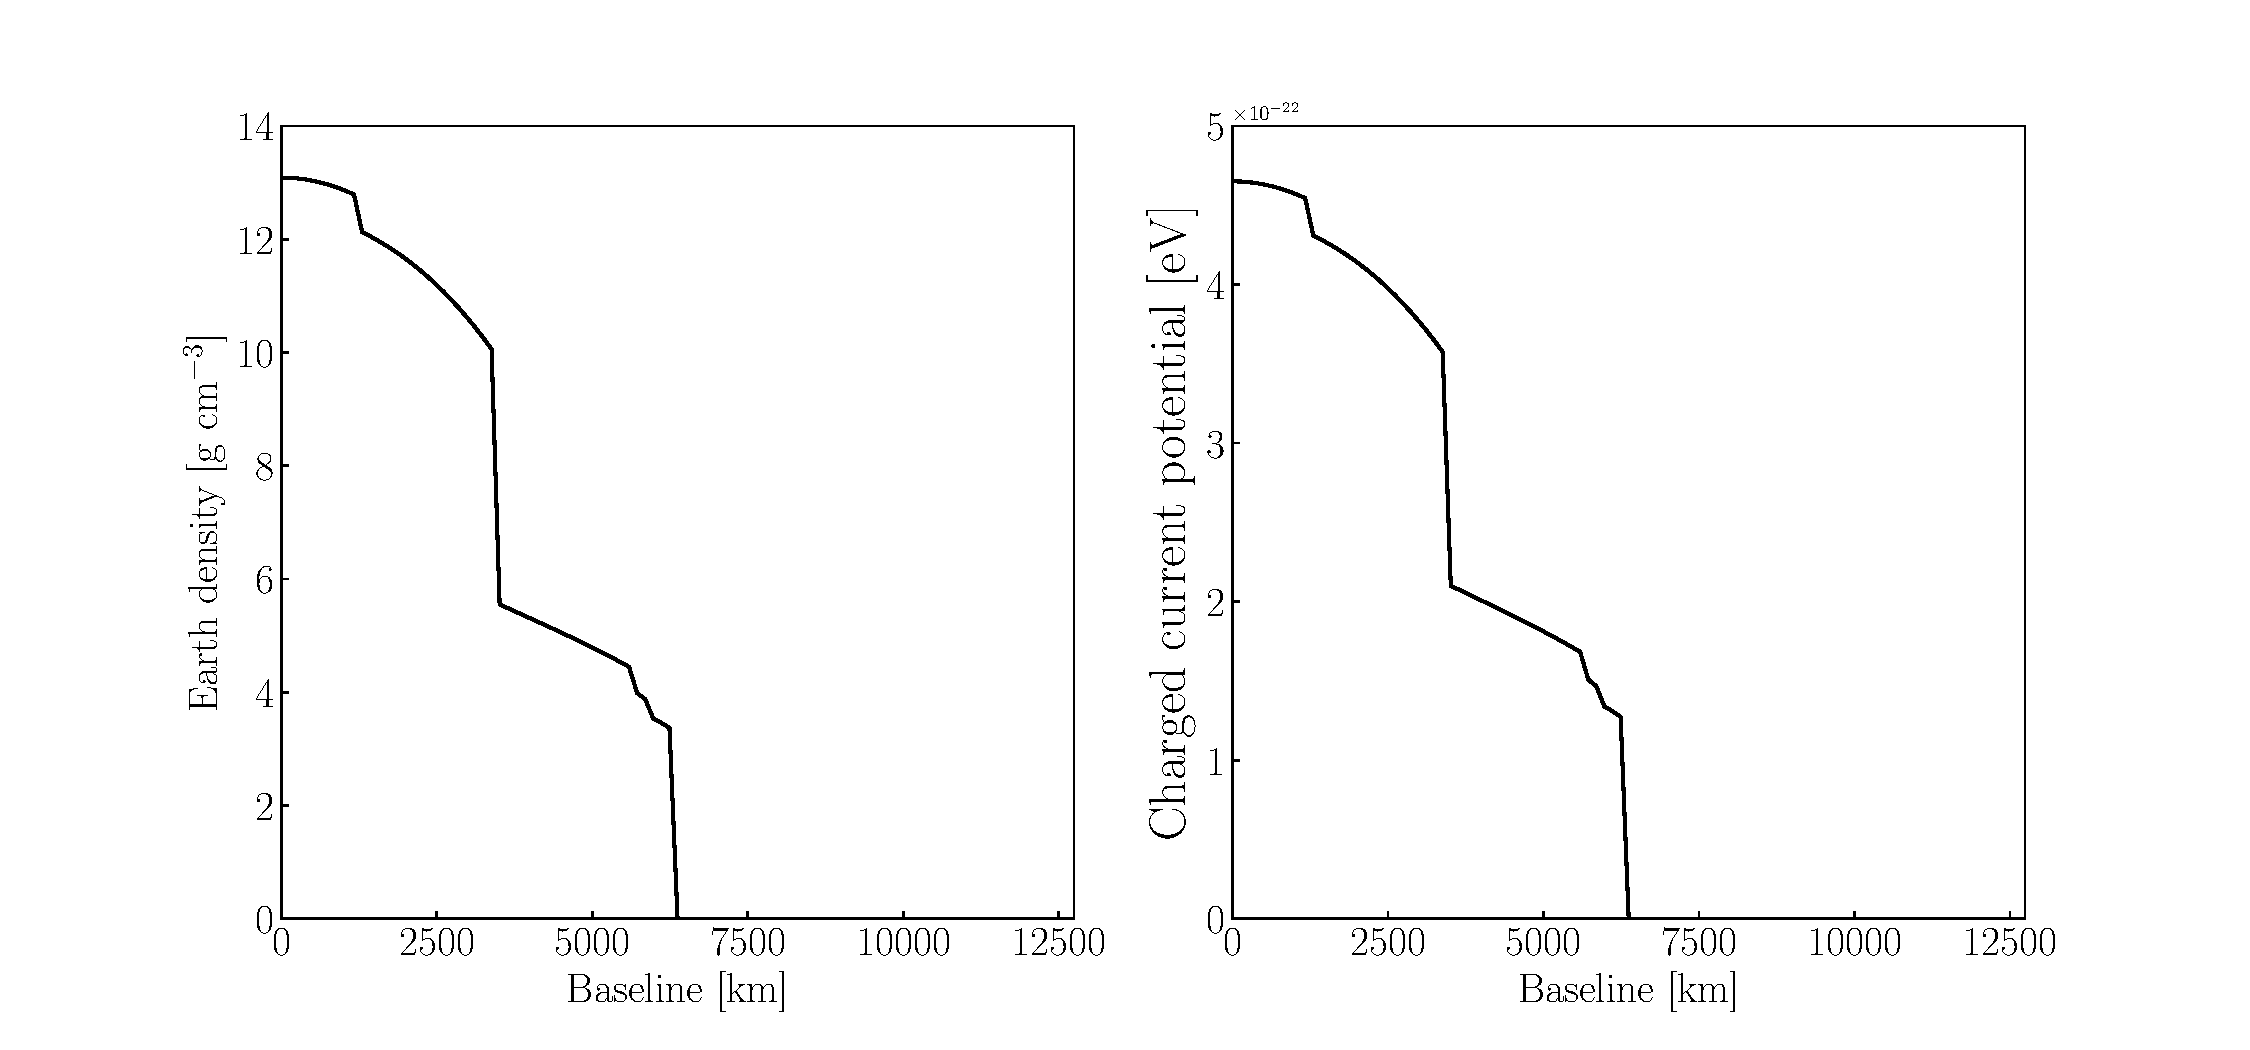
\includegraphics[width=0.7\textwidth]{figures/potential.pdf}
    \caption{\emph{Left panel:} The spherically symmetric Earth density according to PREM~\cite{PREM}, as of distance from the core.
    \emph{Right panel:} $V_{CC}$ using the PREM density and 1/2 electrons per nucleon.}\label{fig:potential}
\end{figure}

Now, solving the Schrödinger equation with the Hamiltonian from Eq.~\ref{eq:H_3gen} with the matter potential from the PREM,
we obtain the nine combinations of probabilities through the Earth diameter. We note that due to our assumption of CP-invariance
(and thus, T-invariance), the probabilities $P_{\a\b}$ and $P_{\b\a}$ are identically equivalent. The result for \si{\GeV} neutrinos 
is shown in Fig.~\ref{fig:oscillations}.

\begin{figure}
    \centering
    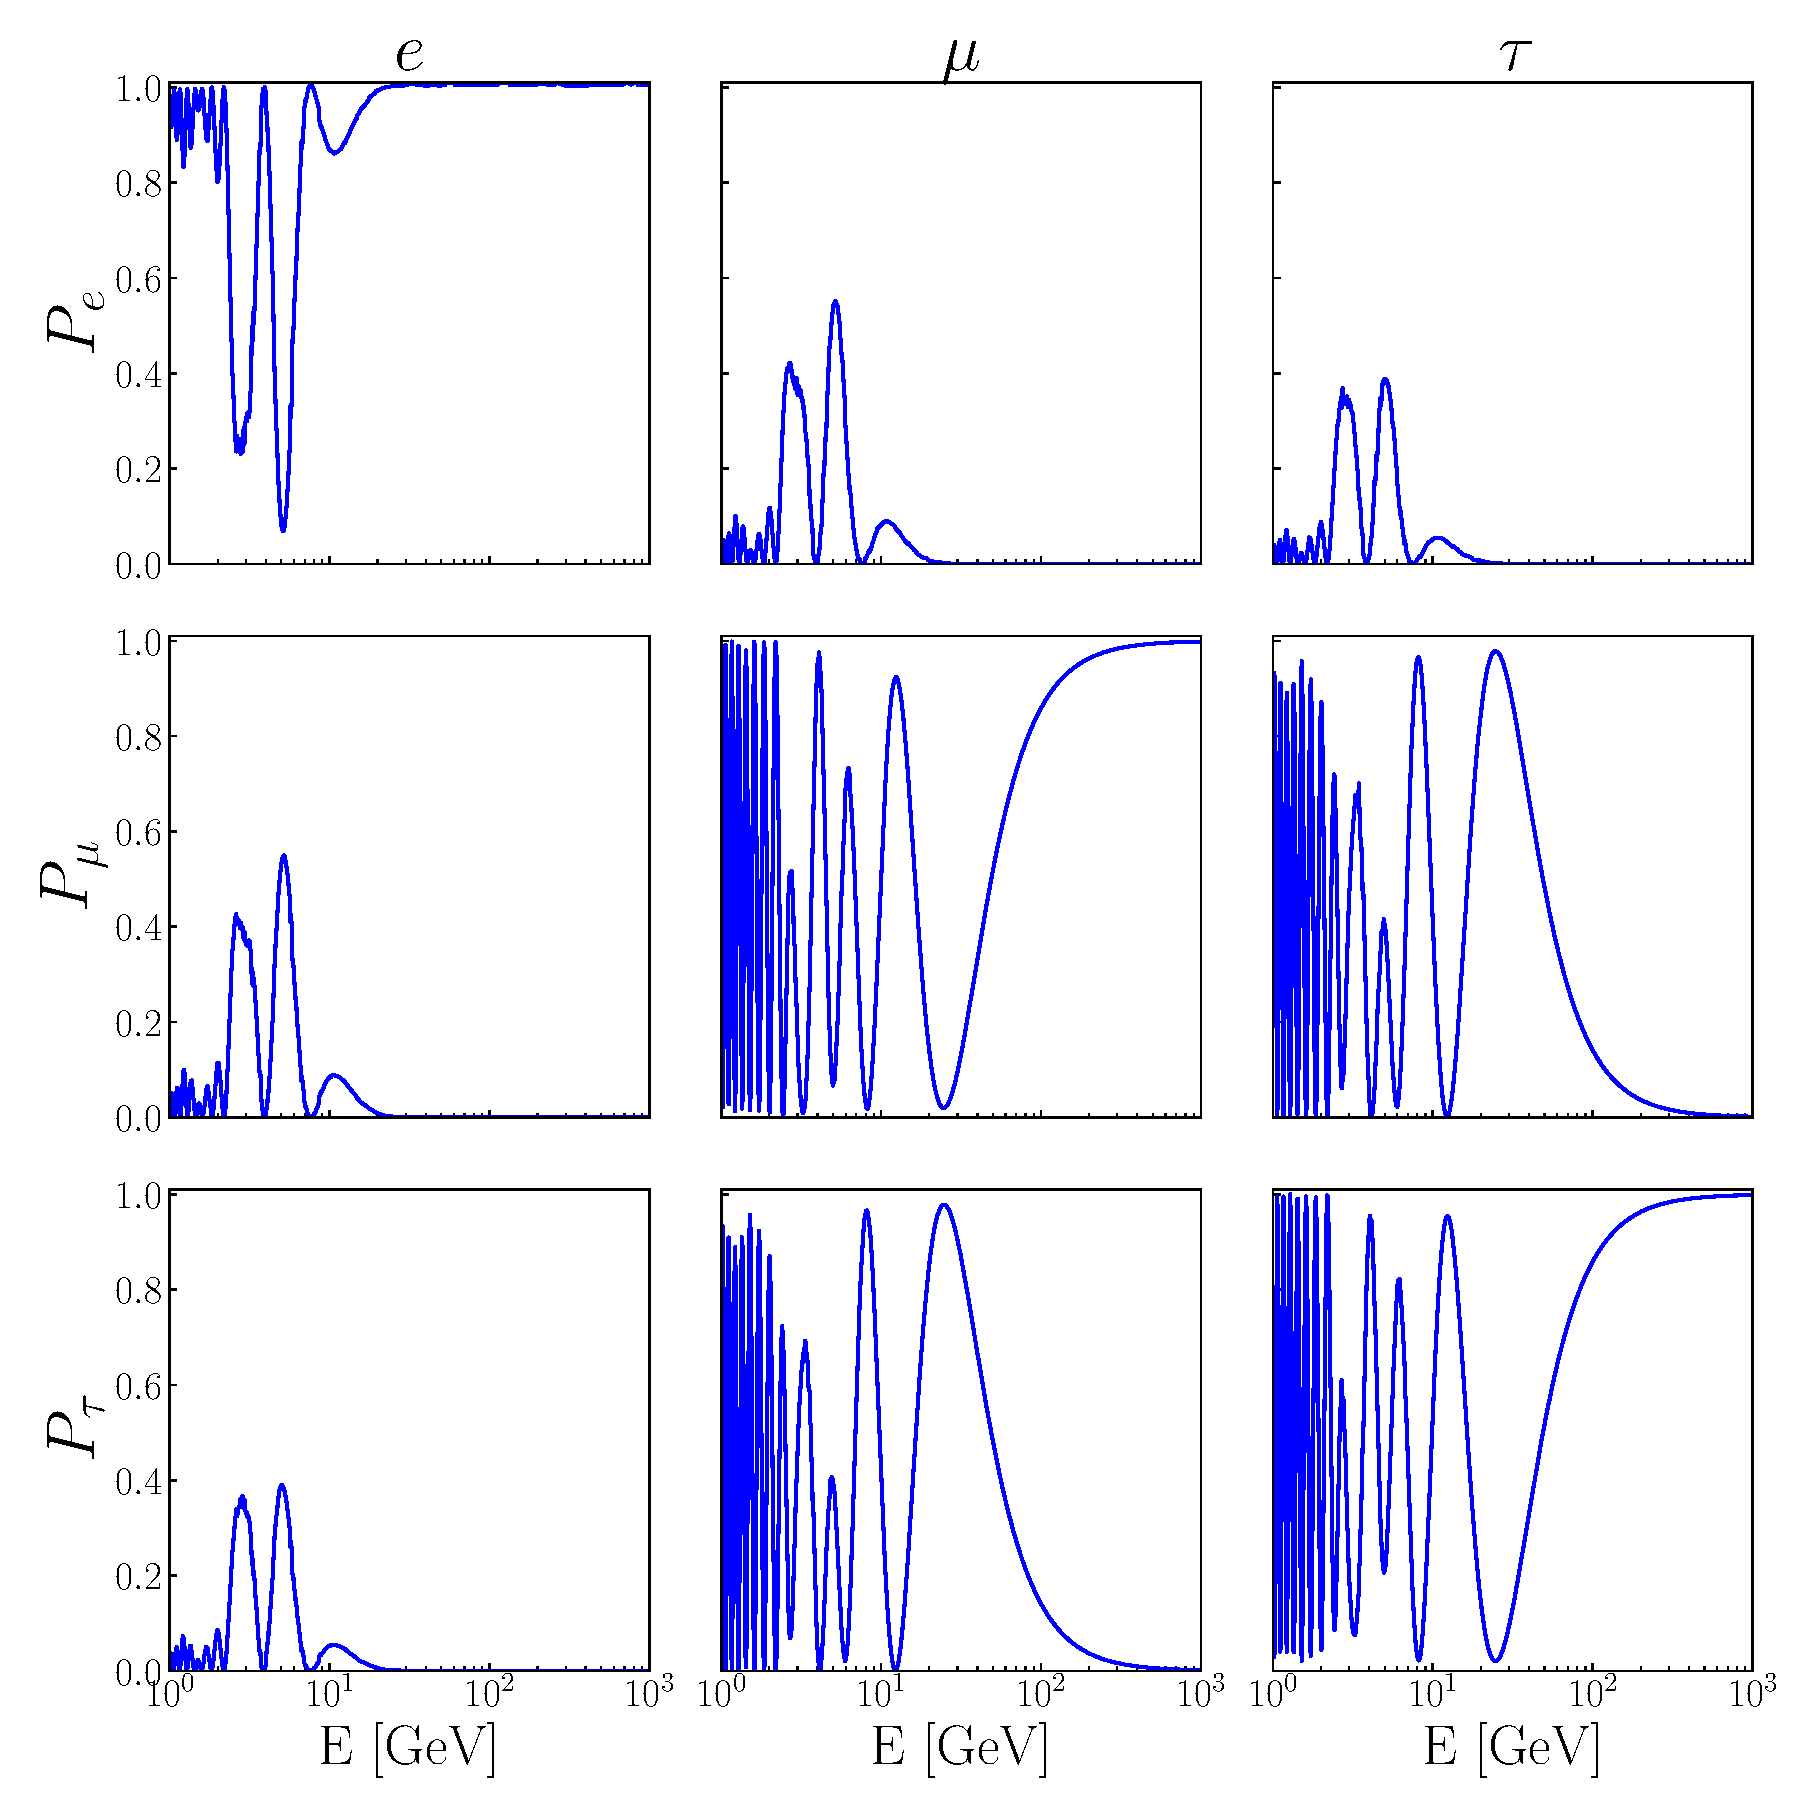
\includegraphics[width=0.7\textwidth]{figures/oscillations.pdf}
    \caption{}\label{fig:oscillations}
\end{figure}

Now we need to incorporate the \emph{zenith angle}, defined as the angle between the neutrino direction of travel and south.
This way, neutrinos traveling through the entire diameter of the Earth up through the South Pole are defined as `up-going', while
neutrinos that start at the South Pole are `down-going'. We will mostly work with the quantity $\cos{(\theta_z)}$.
Since we are interested in the matter effects, we reserve our IceCube study to up-going neutrinos, i.e. neutrinos with
zenith angle $-1<= \cos{(\theta_z)}<=0$. We now supplement our probability grid from Fig.~\ref{fig:oscillations} with the zenith dimension,
allowing us to fully see the Earth matter effect on the oscillations in full. This is shown in Fig.~\ref{fig:oscillograms}.

\begin{figure}
    \centering
    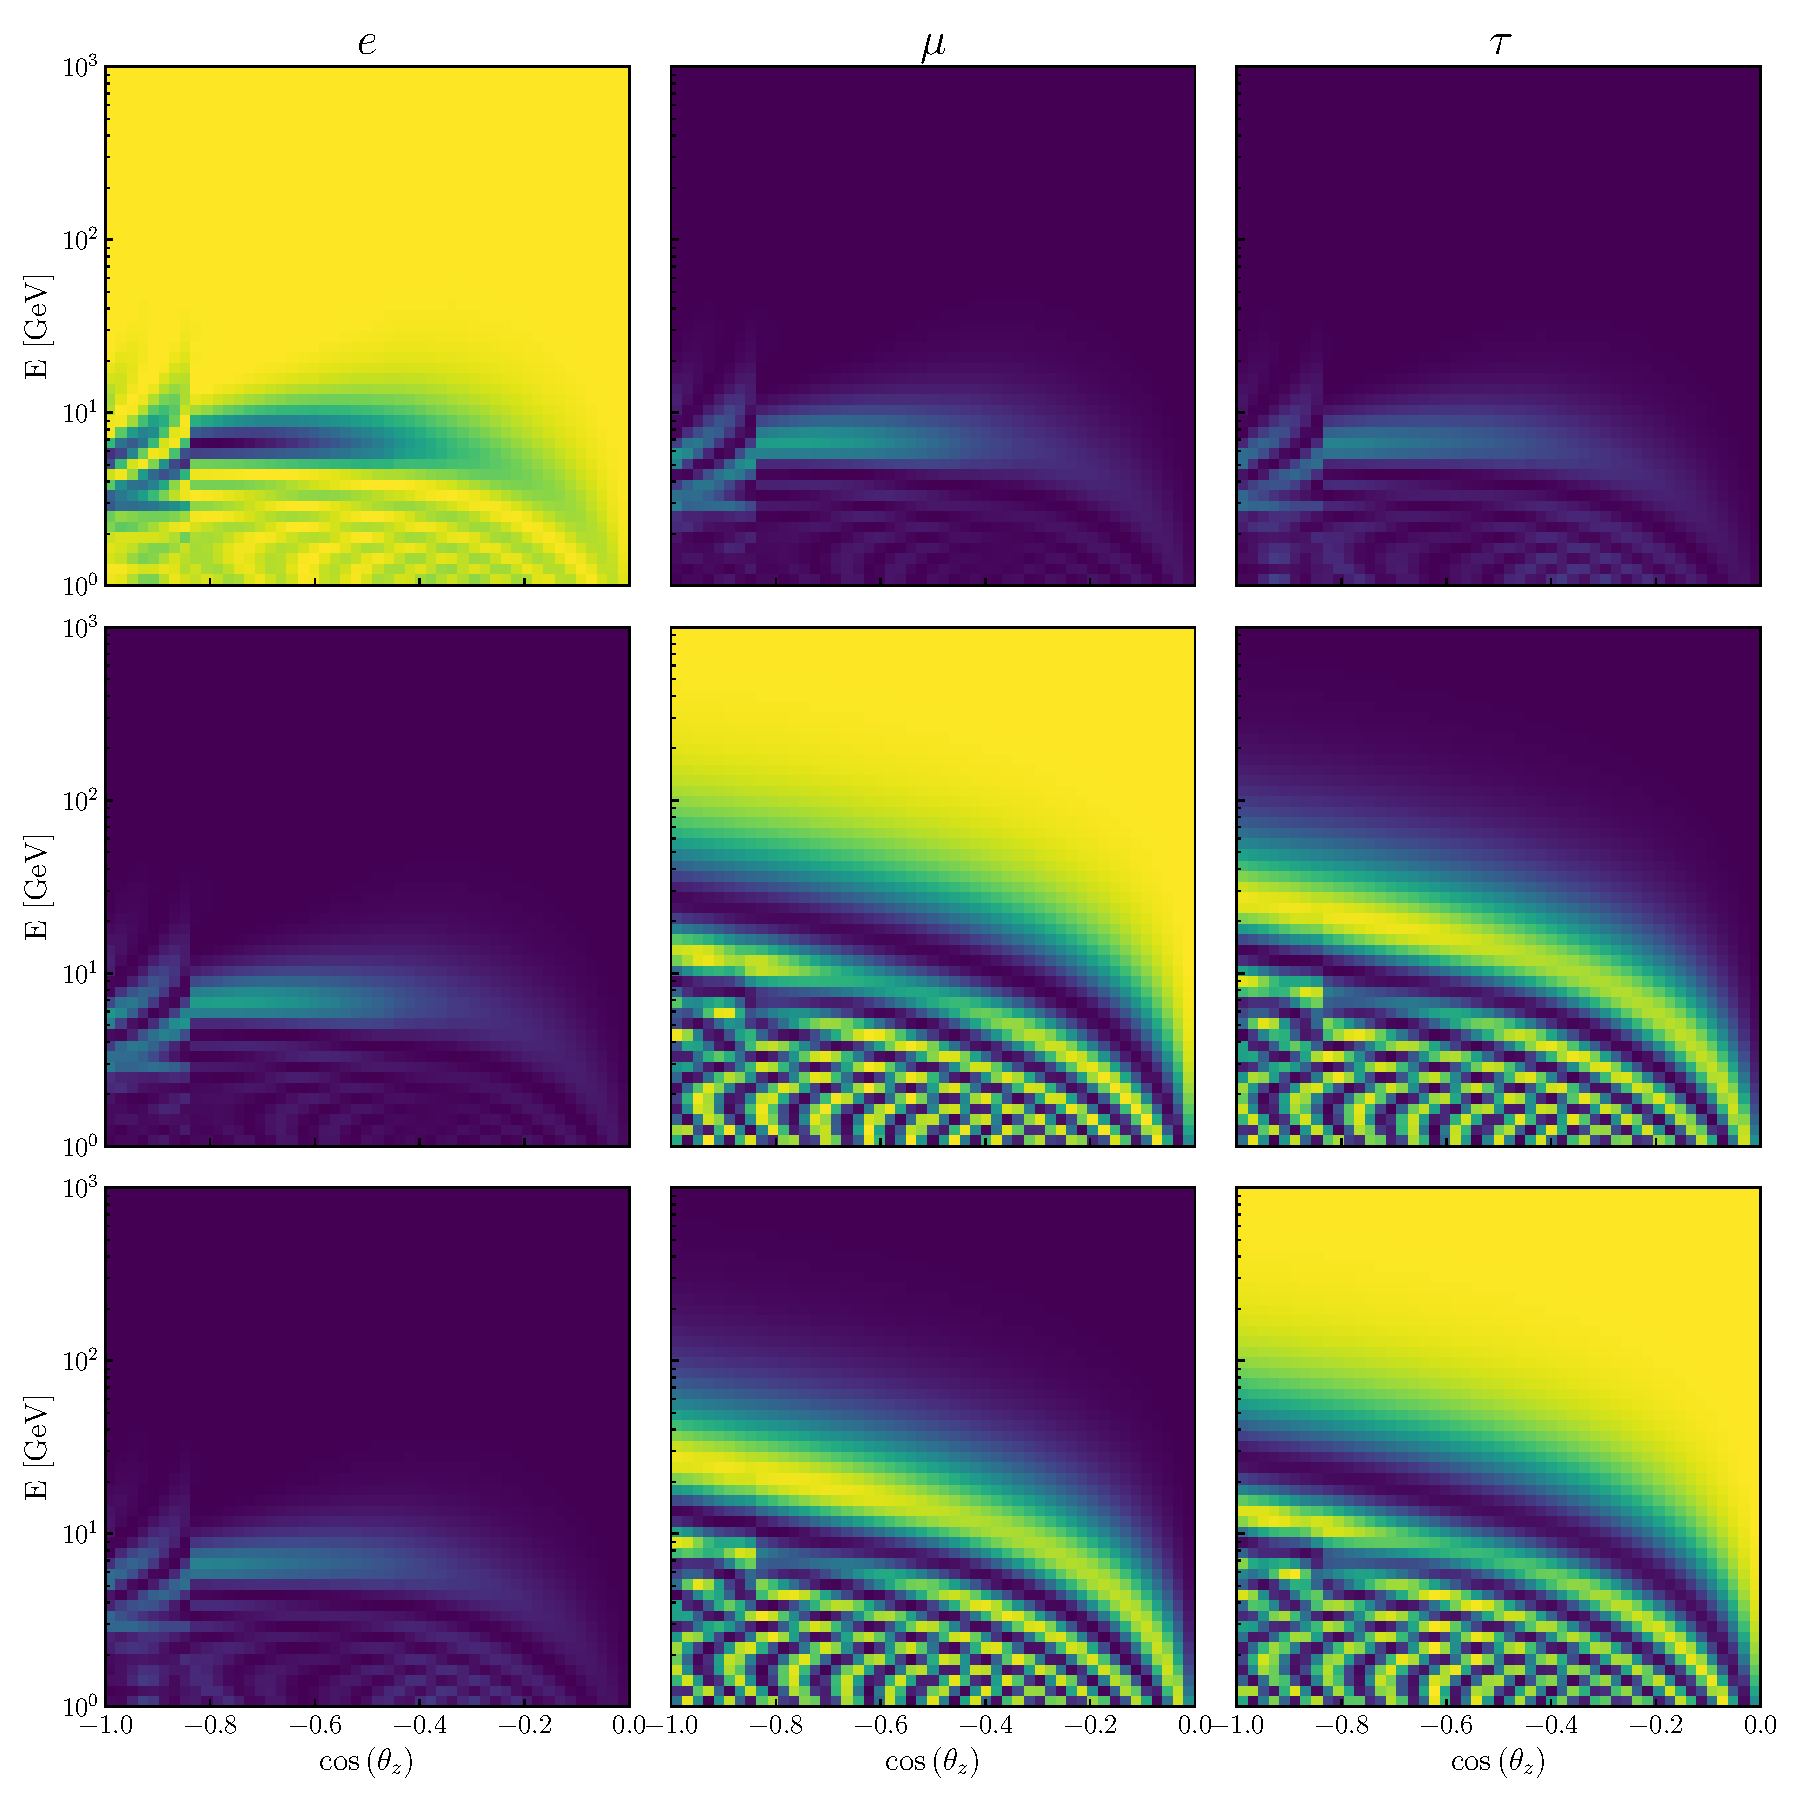
\includegraphics[width=0.7\textwidth]{figures/oscillograms.pdf}
    \caption{Oscillograms showing neutrino oscillations for all flavors in E-$\cos(\theta_z)$ space.}\label{fig:oscillograms}%TODO: redo finer
\end{figure}%TODO: remake with finer
The core-mantle boundary from Fig.\ref{fig:potential} is clearly displayed at $\cos{(\theta_z)} = -0.83$ as a sharp discontinuity for all flavors. 

% \end{document}
\chapter{The Antarctic Detectors}\label{ch:ic}
% \documentclass{thesis}
% \usepackage[margin=0.5in]{geometry}
% \usepackage{graphicx, slashed, siunitx, subcaption}
% \usepackage[utf8]{inputenc}
% \usepackage{xr-hyper}
% \documentclass[a4paper,10pt,draft]{thesis}
\usepackage{physics,amsmath, amsfonts, siunitx, amssymb, graphicx, slashed,subcaption}
\usepackage[utf8]{inputenc}
\usepackage[margin=1in]{geometry}
\usepackage[hidelinks]{hyperref}
\usepackage{xr-hyper}
\newcommand{\n}[1]{\nu_{#1}}
\newcommand{\na}{\nu_\alpha}
\newcommand{\nb}{\nu_\beta}
\newcommand{\ana}{\bar{\nu}_\alpha}
\newcommand{\an}[1]{\bar{\nu}_{\text{#1}}}
\newcommand{\anb}{\bar{\nu}_\beta}
\renewcommand{\a}{\alpha}
\renewcommand{\b}{\beta}
\newcommand{\ab}{\alpha\beta}


\renewcommand{\ne}{\nu_e}
\newcommand{\nm}{\nu_\mu}
\newcommand{\nt}{\nu_\tau}
\newcommand{\ns}{\nu_s}

\newcommand{\ane}{\bar{\nu}_e}
\newcommand{\anm}{\bar{\nu}_\mu}
\newcommand{\ant}{\bar{\nu}_\tau}
\newcommand{\ans}{\bar{\nu}_s}

\newcommand{\nee}{\nu_e \to \nu_e}
\newcommand{\nem}{\nu_e \to \nu_\mu}
\newcommand{\net}{\nu_e \to \nu_\tau}
\newcommand{\nes}{\nu_e \to \nu_s}

\newcommand{\nme}{\nu_\mu \to \nu_e}
\newcommand{\nmm}{\nu_\mu \to \nu_\mu}
\newcommand{\nmt}{\nu_\mu \to \nu_\tau}
\newcommand{\nms}{\nu_\mu \to \nu_s}



\newcommand{\Pee}{P_{e  e}}
\newcommand{\Pem}{P_{e  \mu}}
\newcommand{\Pet}{P_{e  \tau}}
\newcommand{\Pes}{P_{e  s}}

\newcommand{\Pme}{P_{\mu  e}}
\newcommand{\Pmm}{P_{\mu\mu}}
\newcommand{\Pmt}{P_{\mu  \tau}}
\newcommand{\Pms}{P_{\mu  s}}


\newcommand{\Pte}{P_{P_{\tau e}}}
\newcommand{\Ptm}{P_{\tau  \mu}}
\newcommand{\Ptt}{P_{\tau  \tau}}
\newcommand{\Pts}{P_{\mu  s}}

\newcommand{\Paeae}{P_{\bar{e}  \bar{e}}}
\newcommand{\Paeam}{P_{\bar{e}  \bar{\mu}}}
\newcommand{\Paeat}{P_{\bar{e}  \bar{\tau}}}
\newcommand{\Paeas}{P_{\bar{e}  \bar{s}}}

\newcommand{\Pamae}{P_{\bar{\mu}  \bar{e}}}
\newcommand{\Pamam}{P_{\bar{\mu}  \bar{\mu}}}
\newcommand{\Pamat}{P_{\bar{\mu}  \bar{\tau}}}
\newcommand{\Pamas}{P_{\bar{\mu}  \bar{s}}}


\newcommand{\Patae}{P_{\bar{\tau}  \bar{e}}}
\newcommand{\Patam}{P_{\bar{\tau}  \bar{\mu}}}
\newcommand{\Patat}{P_{\bar{\tau}  \bar{\tau}}}
\newcommand{\Patas}{P_{\bar{\mu}  \bar{s}}}

\renewcommand{\th}[1][]{%
  \theta\ifx\\#1\\\else_\text{#1}\fi
}
\newcommand{\thm}[1][]{%
  \theta^\text{M}\ifx\\#1\\\else_\text{#1}\fi
}
\renewcommand{\t}[1]{\text{{#1}}}
\newcommand{\avg}[1]{\left\langle {#1} \right \rangle}
\newcommand*{\dm}[1][]{%
  \Delta m^2\ifx\\#1\\\else_\text{#1}\fi
}
\newcommand{\zreco}{\cos{(\theta_z^{reco})}}
\newcommand{\ztrue}{\cos{(\theta_z^{true})}}
\newcommand{\z}{\cos{(\theta_z)}}
\newcommand{\Ereco}{E^{reco}}
\newcommand{\Etrue}{E^{true}}
\newcommand{\Aeff}{A^\text{eff}}
\newcommand{\emm}{\epsilon_{\mu\mu}}
\newcommand{\emt}{\epsilon_{\mu\tau}}
\newcommand{\eet}{\epsilon_{e\tau}}
\newcommand{\eem}{\epsilon_{e\mu}}
\newcommand{\ett}{\epsilon_{\tau\tau}}
\newcommand{\ep}{\epsilon^\prime}

% \begin{document}
\section{Neutrino detection}
We always observe neutrinos indirectly through their associated charged lepton. Regardless of the type of interaction (charged current via the $W$ boson, or neutral current
via the $Z$), a charged lepton exits with altered properties. The lepton is then detected, and the properties of the neutrino involved in the 
interaction is then deduced. This deduction is obviously imperfect, and this introduces complexities that we will handle in Ch.~\ref{ch:ICmethod}. 

In this work, we only study the detectors handeled by the IceCube collaboration. They are of Cherenkov type, which means that they detect 
the secondary charged lepton by its emitted Cherenkov light, produced from its travel through the Antarctic ice. 
If the charged leptons interact heavily with the ice, they will travel a short distance and emit a localized flash of 
Cherenkov light. This event is referred to as a cascade. The neutral current interactions involves quarks, which recoils and procudes
showers of hadrons. Also, charged current $\ne$ interactions also produce cascades. A cascade event 
is shown in Fig.~\ref{fig:events_cascade}.
If the charged leptons don't interact as much in the ice, they penetrate a larger part of it, emitting light and tertiary particles
as they go. This event is referred to as a track, and are often due to muon charged current interactions. A track event 
is shown in Fig.~\ref{fig:events_track}.

\begin{figure}\label{fig:events}
    \begin{center}
        \begin{subfigure}{0.4\textwidth}
            \centering
            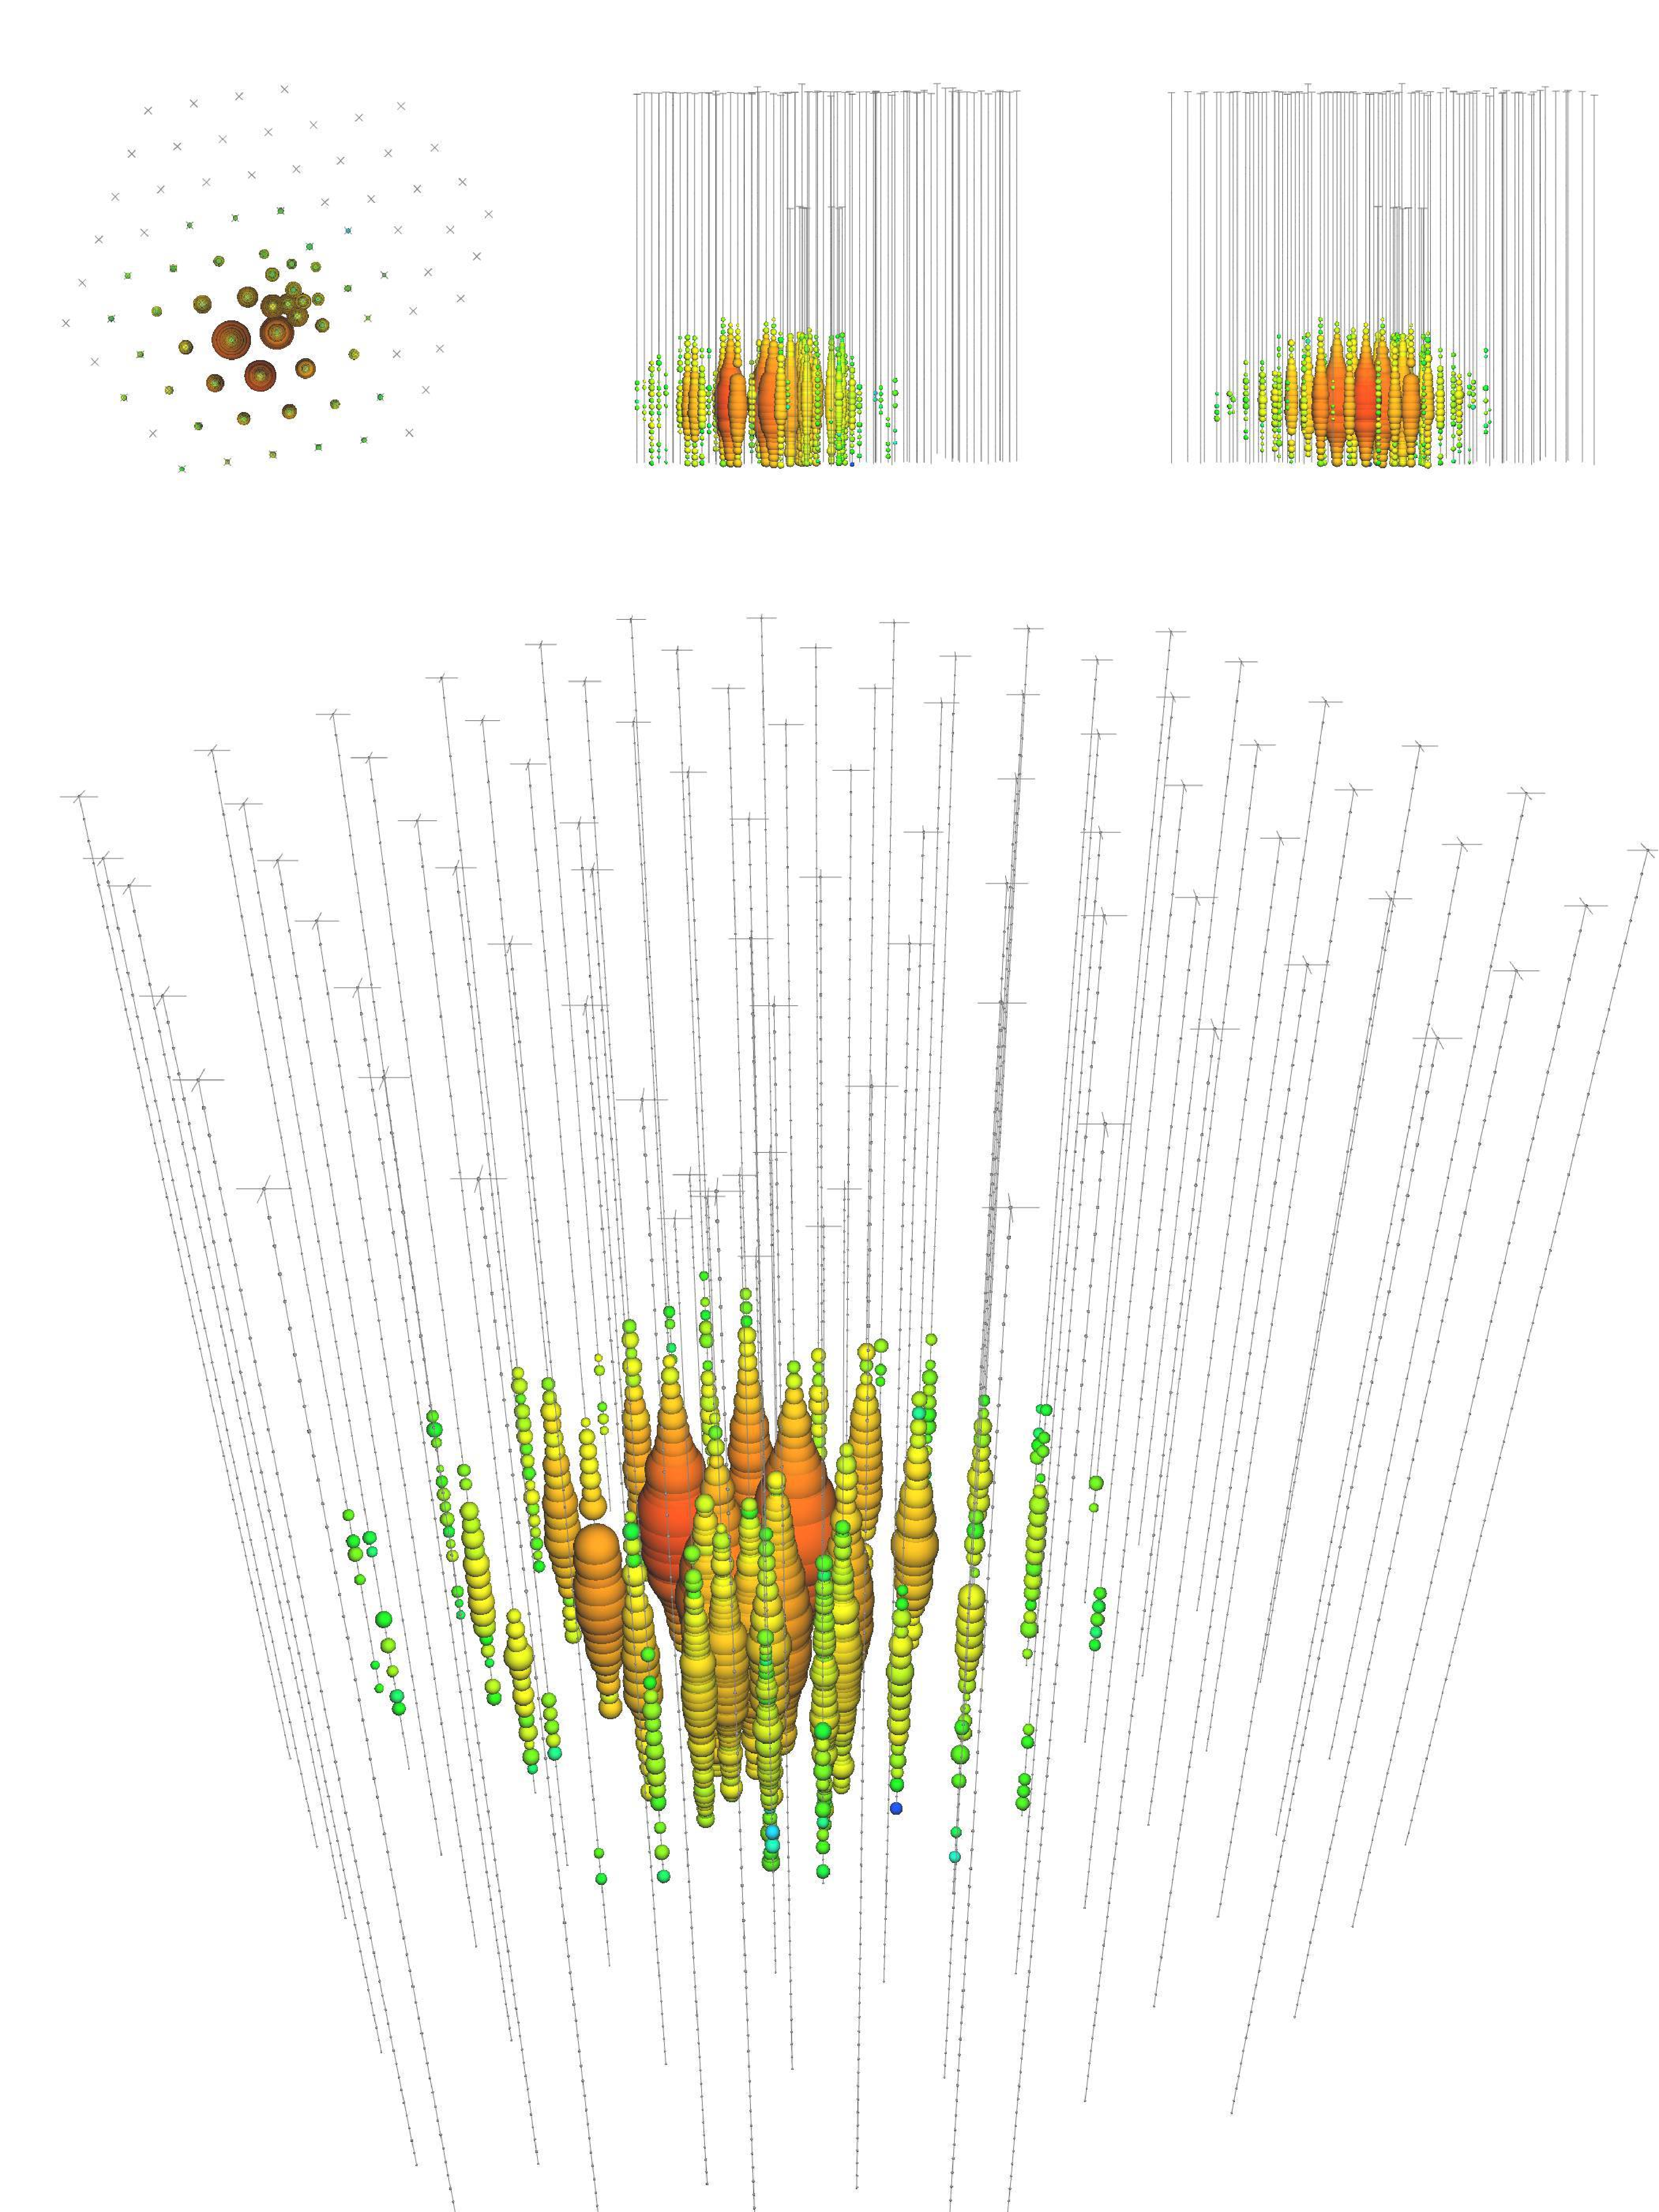
\includegraphics[clip, trim=0cm 0cm 0cm 30cm, width=1\textwidth]{figures/cascade_event.pdf}
            \caption{Event classified as cascade}  
            \label{fig:events_cascade}
          \end{subfigure}
        \begin{subfigure}{0.4\textwidth}
            \centering
            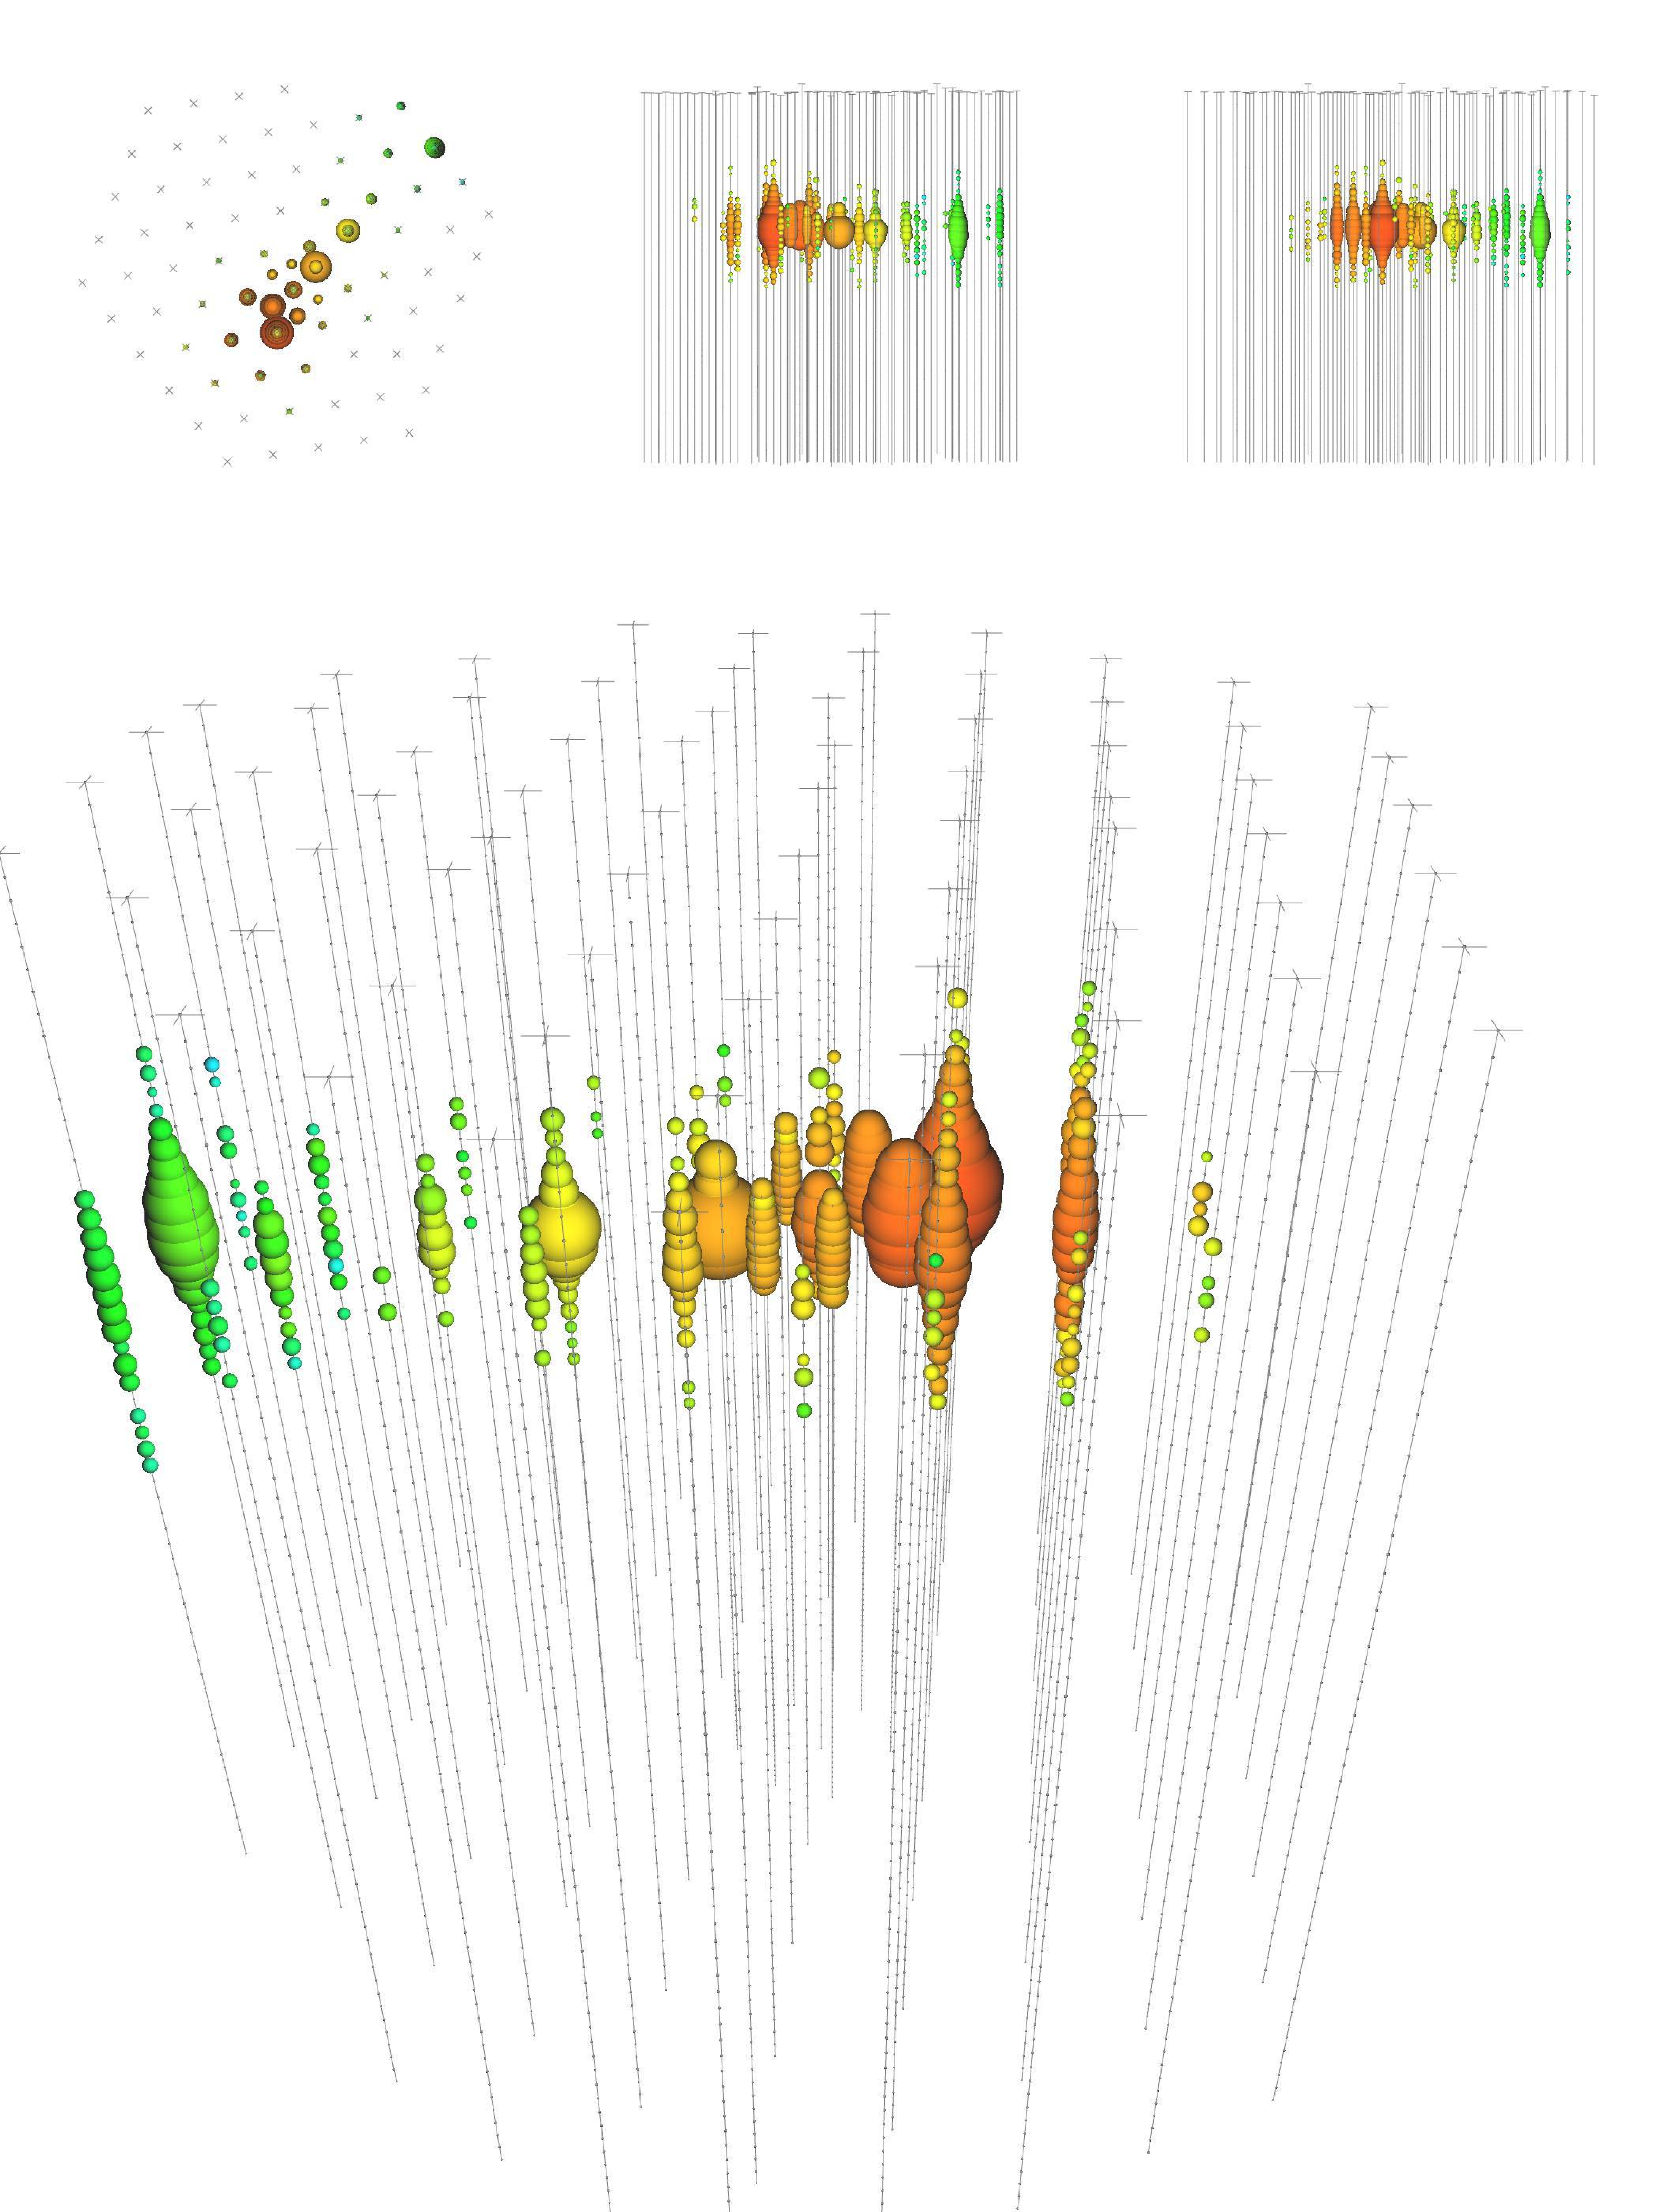
\includegraphics[clip, trim=0cm 0cm 0cm 30cm, width=1\textwidth]{figures/track_event.pdf}
            \caption{Event classified as track} 
            \label{fig:events_track}
        \end{subfigure}
        \caption{The two event types distinguished in the IceCube detector.}
    \end{center}
\end{figure}

To detect the Cherenkov light, 60 Digital Optical Modules (DOMs) are placed on a long string up to \SI{17}{\metre} apart. 86 of these strings are then lowered
into \SI{2.5}{\km} deep boreholes in the ice. The holes are then sealed by refreezing the ice, resulting in a total of 5160 DOMs in a volume of approximately \SI{1}{\km^3}~\cite{weaverThesis}.
%TODO: pic of cherenkov light/dom?

The strings and DOMs are not spaced evenly, making some parts of the detector more sensitive to certain energy ranges than other.
8 strings packed more tightly than the other 78, making that part of the detector sensitive to neutrino energies down to single digit \si{\GeV}. Due to 
this part being situated deep within the ice, it is referred to DeepCore. DeepCore will be treated as a separate and independent detector from the rest, which
retains the name IceCube. A view of the current setup can be seen in Fig.~\ref{fig:array}. In this work, we consider DeepCore data between \SIrange{5.6}{56}{\GeV} and IceCube data in the range \SIrange{0.5}{10}{\TeV}.
\begin{figure}\label{fig:array}
    \centering
    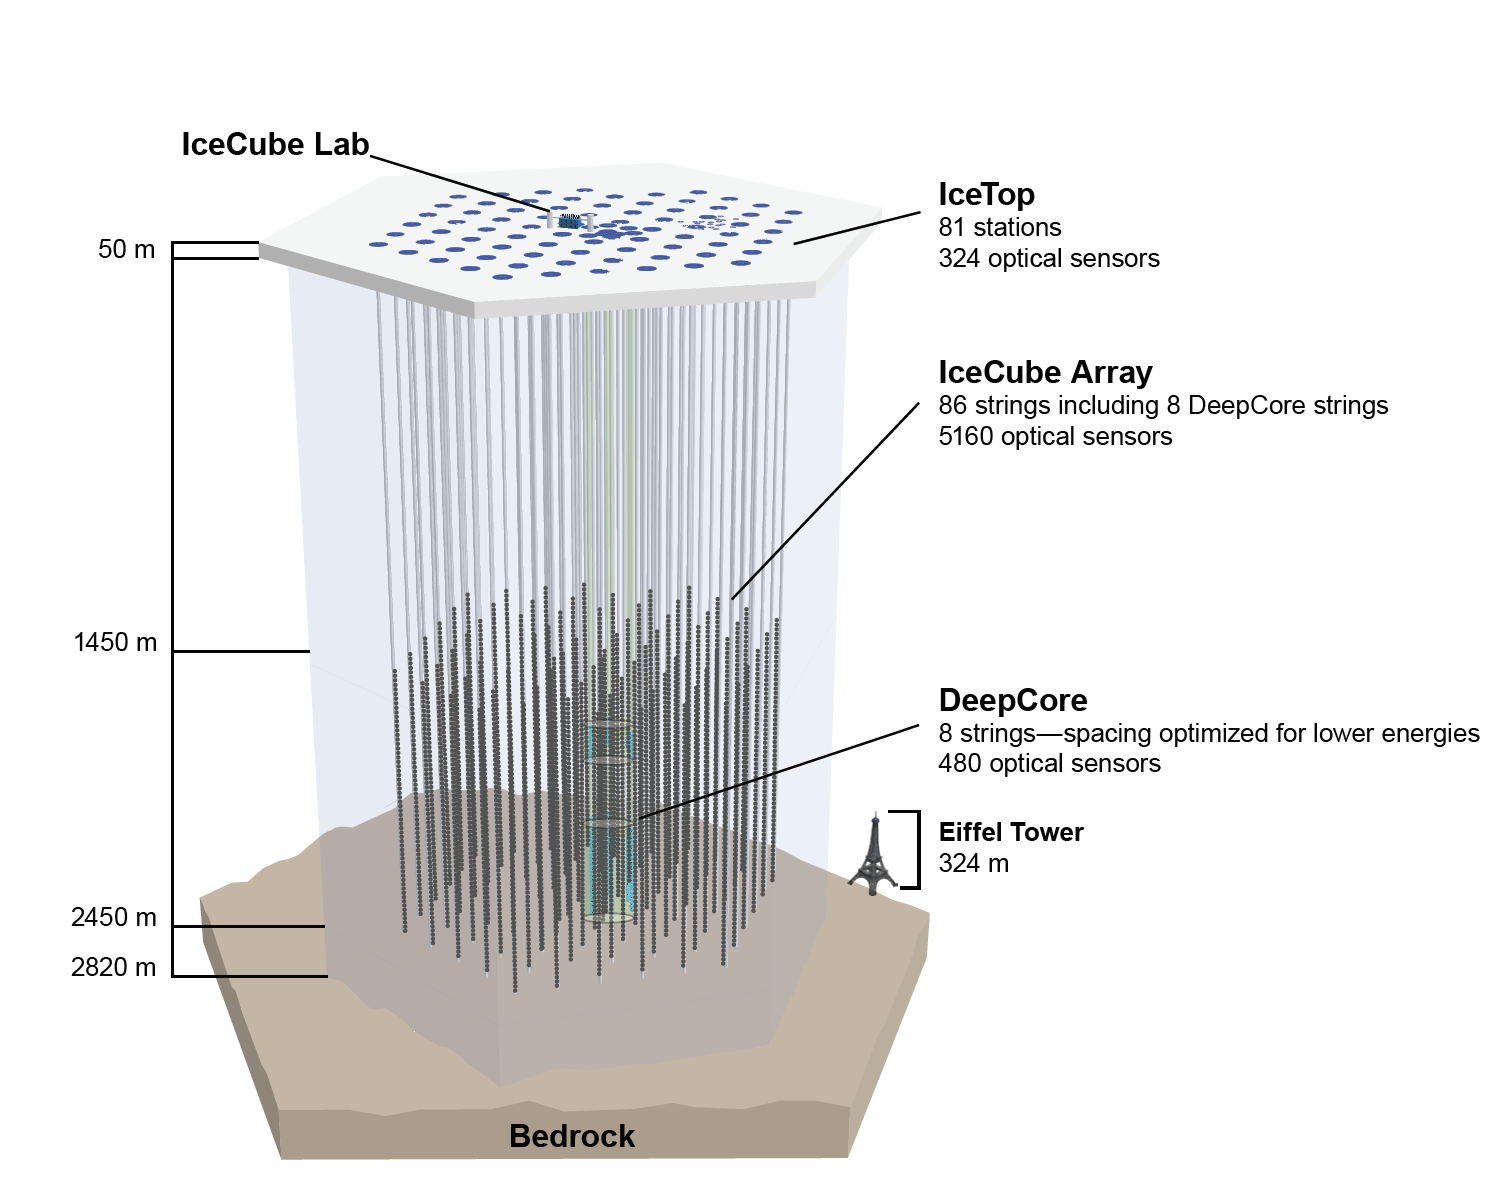
\includegraphics[width=0.5\textwidth]{figures/icecube2.png}
    \caption{View of the full IceCube array}
\end{figure}

In 2017, the PINGU Letter of Intent was published~\cite{PINGUletter}. The `Precision IceCube Next Generation Upgrade' is an upgrade that will 
supplement DeepCore, i.e. boosing the capabilites of neutrino detection at the \si{\GeV} scale. As the PINGU upgrade is not yet financed nor built, we are
not able to use any data from it. However, the collaboration has released preliminary simulations which we will use to see how the upgrade might improve
IceCube and DeepCore bounds. The PINGU simulations have the same structure as the DeepCore data, so any analysis referring to DeepCore will
also apply to PINGU except where noted. However, we treat the PINGU detector as independent of the DeepCore experiment.

\begin{figure}[t]\label{fig:flux_aeff}
    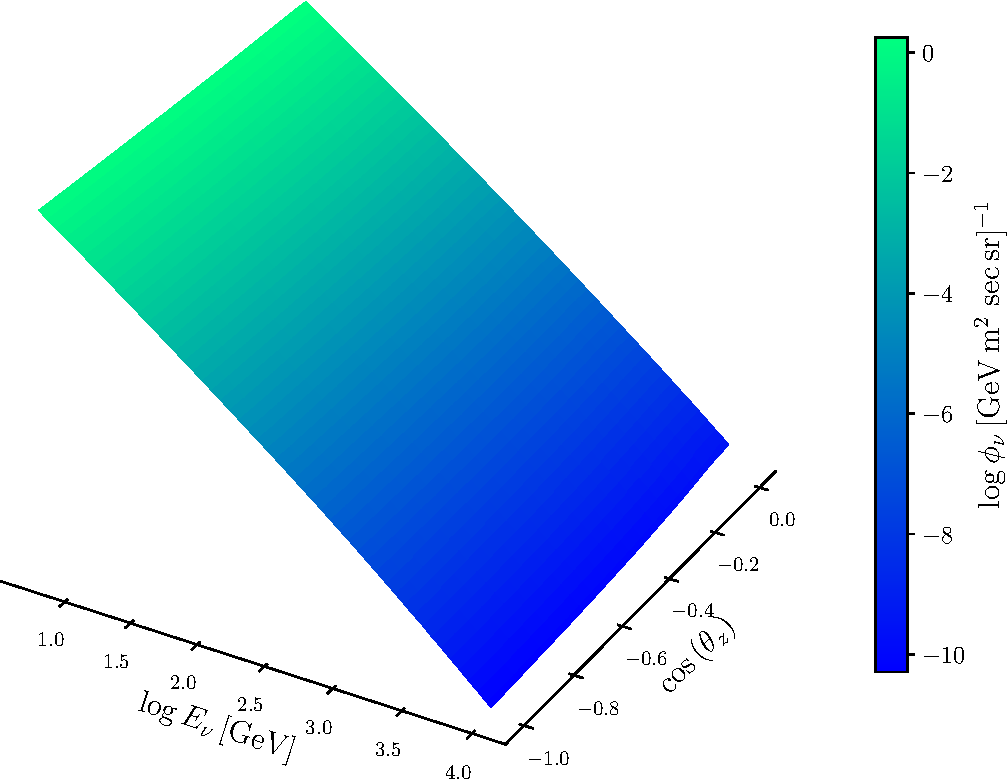
\includegraphics[width=0.5\textwidth]{figures/flux.pdf}\hspace{-1cm}
    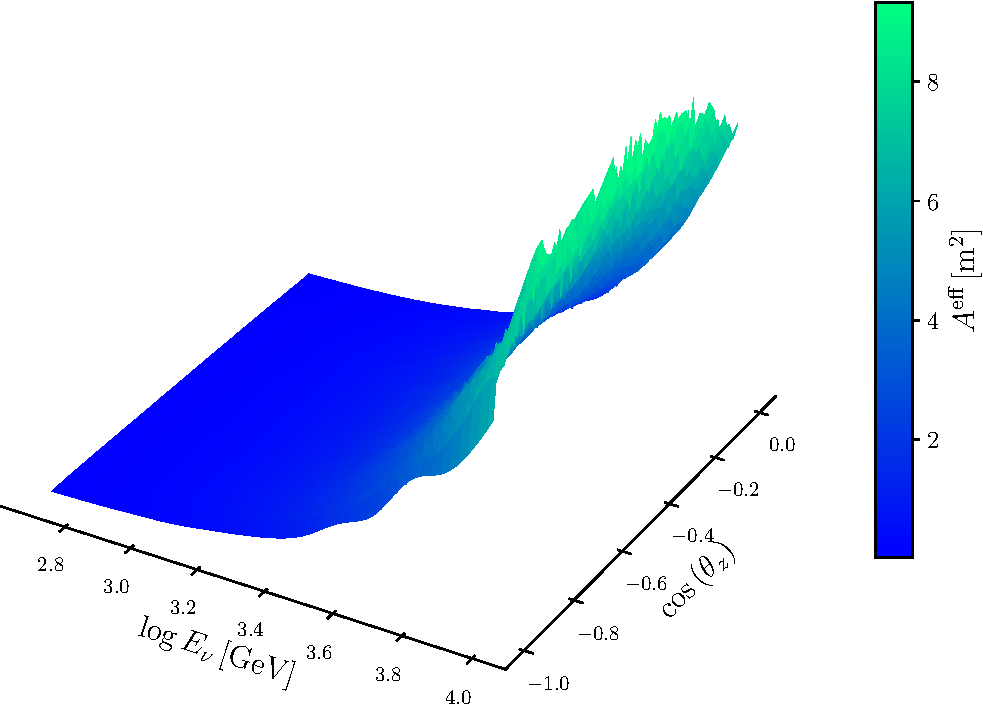
\includegraphics[width=0.5\textwidth]{figures/aeff.pdf}
    \vspace{-2.5cm}\caption{\emph{Left panel:} Interpolated South Pole atmospheric flux with data from~\cite{hondaArticle}.
    \emph{Right panel:} Interpolated IceCube effective area with data from~\cite{ICaeff}.}
\end{figure}

\subsection{Atmospheric neutrino flux}
Atmospheric neutrinos originates from cosmic rays composed of protons interacting with nuclei in the atmosphere.
These interactions ultimately produces pions, which decay as 
\begin{align}\label{eq:pion}
    &\pi^+ \to \mu^+ + \nm\,, \quad \pi^- \to \mu^- + \anm \nonumber \\
    &\pi^+ \to e^+ + \ne\,,\,\, \quad \pi^- \to e^- + \ane\,.
\end{align}
In the muonic decay channel, muons are emitted which will be detected by the IceCube detector. A part of the 
uncorrelated systematic error comes from this \emph{muon background}, i.e. events misclassified as muons from 
$\nm$ interactions rather than from pion decay. Moreover, the atmospheric flux is often associated with a large error.
In this work, we will use a flux normalization error of 24\%, and a zenith slope error of 4\%~\cite{hondapaper}.

The flux is provided in \cite{hondaData,hondaArticle}, and a selection is shown in Table~\ref{table:flux}
The flux data is binned in $\ztrue$. The fluxes are averaged over azimuthal direction and over solar minimum/maximum. 
The units of the fluxes are given as \si{\per\GeV \per\metre\squared \per\second \per\steradian} and are omitted
from the table for clarity. 
We note that the fluxes for $\nt$ and $\nu_{\bar{\tau}}$ are missing. Kaons can decay into neutral pions, which in turn 
can produce $\nt$, but this branching ratio is extremely small. Thus, we never have to use probabilities on the form 
$P_{\tau \beta}$, since we have no incoming atmospheric $\nu_\tau$ flux. 
Interpolating the data yields makes us capable of returning all four necessary fluxes for a given true energy and true zenith.
The result is shown in Fig.~\ref{fig:flux_aeff}.

\begin{table}[h]\label{table:flux}
    \begin{center}
        \begin{tabular}{lcccccc}
            \hline \hline
            $\Etrue$ [\si{\GeV}] &$\phi_\mu$ &$\phi_{\bar{\mu}}$ &$\phi_e$ &$\phi_{\bar{e}}$ & $\ztrue$\\\\
            \hline
            27825 &  \SI{6.06e-12}{} &  \SI{3.17e-12}{} &  \SI{1.56e-13}{} &  \SI{1.04e-13}{} &   [-0.2, -0.1] \\
            247707 &  \SI{5.94e-16}{} &  \SI{2.92e-16}{} &  \SI{1.36e-17}{} &  \SI{8.12e-18}{} &   [-0.7, -0.6] \\
                22 &  \SI{3.33e-02}{} &  \SI{2.78e-02}{} &  \SI{9.57e-03}{} & \SI{7.15e-03}{} &   [-0.3, -0.2] \\
            432876 &  \SI{5.19e-17}{} &  \SI{2.32e-17}{} &  \SI{1.46e-18}{} & \SI{9.83e-19}{} &   [-1.1, -1.0] \\
            64280 &  \SI{1.58e-13}{} &  \SI{8.10e-14}{} &  \SI{3.49e-15}{} &  \SI{2.21e-15}{} &   [-0.4, -0.3] \\
            \hline \hline
        \end{tabular}
    \end{center}
    \caption{A selection of processed atmospheric South Pole fluxes from~\cite{hondaData} by Honda et al.~\cite{hondaArticle}.}
\end{table}


\subsection{Event reconstruction}
After an event has occurred, the IceCube algorithms process the data coming from the detector to \emph{reconstruct} the event. This means that, given the parameters recorded by the detector, what are their "true" values?
We are interested in two variables: the energy and the direction. Each event is tagged with a probable energy and zenith angle, called the recostructed parameters $\Ereco$ and $\zreco$, which are the parameters according to the DOMs.
The collaboration then uses numerous sophisticated methods to backtrack the reconstructed parameters to the true parameters. So a charged lepton hits the DOMs, and we ultimately end up with the associated neutrino's true and reconstructed energy and zenith angle. The reconstructed parameters are what we are using to analyze the data (because this is what the detector actually sees), while the true parameters are used in the determination of that neutrino's "actual" flux and cross-section (because this is what nature sees).

How do we then translate between the reconstructed and true parameters? In this work, we are using two different methods, which are based on the form of data available to us. They will be outlined in Sec.\ref{ch:ICmethod} and Sec.~\ref{ch:DCmethod}.



% \bibliographystyle{nature}
% \bibliography{ref.bib}
% \end{document}
\section{IceCube}\label{ch:ICmethod}
As the neutrinos have propagated the Earth, they arrive at the South Pole, where they interact with charged leptons in the ice. The charged lepton then emits the Cherenkov light detected by the array.
We construct the event rate for each bin as
\begin{align}\label{eq:ICevents}
    N_{ij} &= T \sum_\beta\int_{(\cos{\theta_z^r})_i}^{(\cos{\theta_z^r})_{i+1}} \dd \cos{\theta^r_z} \int_{E^r_{j}}^{E^r_{j+1}} \dd E^r 
    \int_0^\pi R(\theta^r,\theta^t) \dd \cos{\theta^t} \int_0^\infty R(E^r,E^t) \phi_\beta^\text{det}  A^\text{eff}_\beta \dd E^t
    \,,
\end{align}
where $T$ is the live time of the detector, $\beta$ the final neutrino flavors, $\theta_z^r$ the reconstructed 
zenith angle, i.e.~the deduced direction of the incoming neutrino binned with index $i$. $\theta^t_z$ is the true zenith angle, i.e.~the actual direction of the incoming neutrino. 
$E^r$ is the reconstructed energy, binned with index $j$. $R(\theta^r,\theta^t)$ is a zenith resolution function 
that describes the relationship with the reconstructed and true zenith angles, specific to the 86-string configuration of IceCube.
$R(E^r,E^t)$ is an energy resolution function 
that describes the relationship with the reconstructed and true energies. $\phi_\beta^\text{det}$ is the conventional atmospheric neutrino flux for flavor $\beta$, propagated to detector level
in accordance with Eq.~\ref{eq:propFlux}.

We now are interested in the effective area $\Aeff$, 
i.e.~the cross-sectional area of the detector that the lepton is exposed to.
$\Aeff$ depends on several parameters, some of them being physical detector volume, $\Etrue$, $\ztrue$, and the particle type. 
Fortunately, the binned $\Aeff$ is provided to us by the collaboration~\cite{ICaeff}.
An excerpt from this data is shown in Table~\ref{table:aeff}.

\begin{table}[ht]
    \centering
    \begin{tabular}{lrrrrr}
        \hline \hline
        $\Etrue_{min}$ [\si{\GeV}] &     $\Etrue_{max}$ [\si{\GeV}]&   $\ztrue_{min}$ &   $\ztrue_{max}$ &     $\Aeff$ [\si{\metre\squared}] \\
        \hline
             251 &      316 &  -0.92 &  -0.91 &   0.0174 \\
          794300 &  1000000 &  -0.80 &  -0.79 &  69.3600 \\
            3981 &     5012 &  -0.78 &  -0.77 &   3.1490 \\
            1585 &     1995 &  -0.07 &  -0.06 &   0.4659 \\
            398 &      501 &  -0.73 &  -0.72 &   0.0555 \\
        \hline \hline
        \end{tabular}
    \caption{IceCube-86 effective area from~\cite{ICaeff}.}
    \label{table:aeff}
\end{table}

Here, $\Aeff$ has been averaged over $\Aeff_\mu$ and $\Aeff_{\bar{\mu}}$ by the collaboration. Thus, both $\mu$ and $\bar\mu$ will, on average, experience the same $\Aeff$ in our model. 
Just as with the fluxes, we interpolate this in $\Etrue$ and $\ztrue$, and show the result in Fig.~\ref{fig:aeff}
Since the IceCube array is slightly rectangular, the zenith angle affects the cross-sectional area to which the array the leptons are exposed to.
While the flux was almost flat in $\ztrue$, the introduction of the zenith dependent $\Aeff$ will make the result slightly more zenith dependent than the flux itself. 
Increasing linearly with energy, the effective area of the detector approaches its geometrical area of \SI{1e6}{\metre^2} but is still only in the single-digit range at \si{\TeV} energies.

\begin{figure}[ht]%TODO: fix whitespace
    \centering
    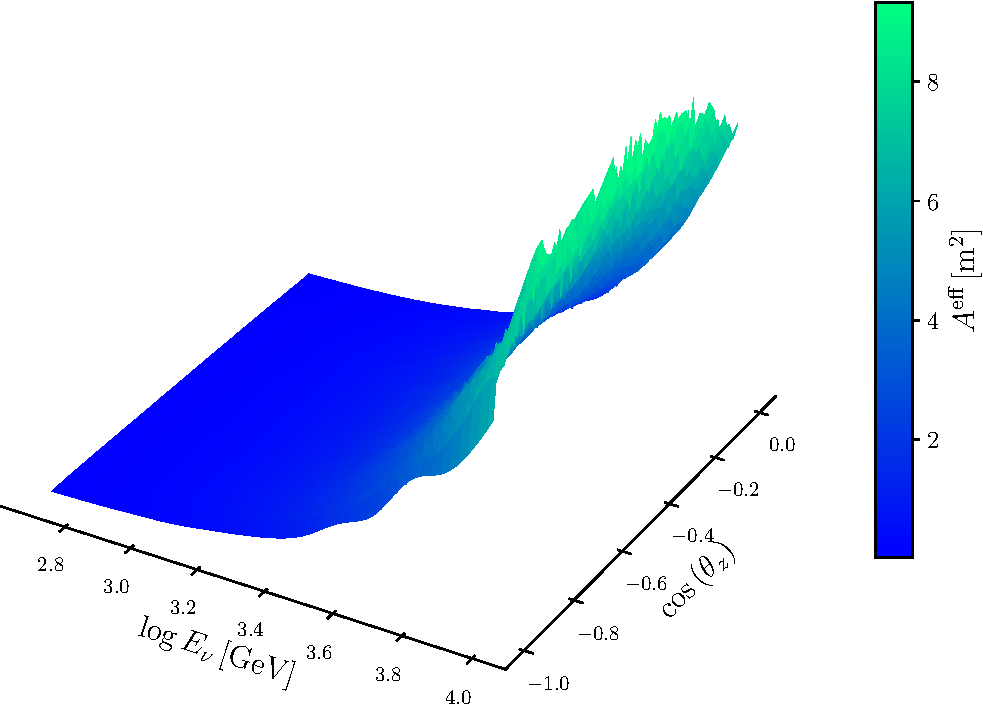
\includegraphics[scale=0.6]{figures/aeff.pdf}
    \caption{Interpolated IceCube effective area with data from~\cite{ICaeff}.}
    \label{fig:aeff}
\end{figure}

So now we have the physical quantities in the true parameters. 
As we discussed, we need a way to translate this into the reconstructed parameters that the detector gives us. We will call the relationship between 
$\Ereco$ and $\Etrue$ the energy resolution function, and the relationship between $\zreco$ and $\ztrue$ the zenith resolution function. 
We assume the relationship to follow a logarithmic Gaussian distribution, giving it the form 
\begin{align}\label{eq:gaussian}
    R(x^r, x^t) = \frac{1}{\sqrt{2\pi} \sigma_{x^r}x^r} \exp\left[-\frac{(\log x^r-\mu(x^t))^2}{2\sigma_{x^r}^2}\right]\,.
\end{align}
The parameters of the Gaussian are $\sigma_{x^r}(x^t)$ and $\mu(x^t)$, which are functions of the true parameters. By multiplying the Gaussian in Eq.~\ref{eq:gaussian}, we are reweighing the values by the 
probability density of that point. This process is also called \emph{smearing} because it effectively spreads out the data around a certain point. 

So how do we then obtain $\sigma_{x^r}(x^t)$ and $\mu(x^t)$ needed to construct the Gaussian? A Monte Carlo sample publicly released by the 
collaboration has all the ingredients that we need~\cite{IC2016}. In Table.~\ref{table:IC_MC} we show a selection of the data.
The `pdg' column refers to the Monte Carlo particle classification, where 13 is the tag for $\nm$, while -13 refers
to an $\anm$. Here we note a crucial property of the IceCube dataset that will impact our analysis: the MC released by the collaboration
only includes simulated muon events.

\begin{table}[ht]
    \centering
    \begin{tabular}{lrrrrr}
        \hline \hline
        pdg &      $\Ereco$ [\si{\GeV}] &     $\zreco$ &       $\Etrue$ [\si{\GeV}] &     $\ztrue$ \\
        \hline
         13 &  1665 & -0.645884 &    592 & -0.653421 \\
         13 &   587 & -0.373241 &    342 & -0.424979 \\
        -13 &  1431 & -0.177786 &   1169 & -0.189949 \\
        -13 &   831 & -0.807226 &   1071 & -0.805559 \\
         13 &   988 & -0.370746 &   1861 & -0.367922 \\
         \hline \hline
  \end{tabular}
  \caption{A selection of the data found in~\cite{IC2016}}
  \label{table:IC_MC}
\end{table}

First, we let $\zreco = \ztrue$ for all values. The angular resolution in IceCube for track-like events is less than $\SI{2}{\degree}$, making $\ztrue$ coincide with $\zreco$ for our study~\cite{IC2020}.
Thus, we only need to concern ourselves with the energy resolution function.
In Fig.~\ref{fig:IC_MC_gpr}, we have plotted all event counts found in the MC file, over 8 million. However, this is too much data to process efficiently, with many outliers that ultimately do not weigh in 
that much in the final event count. To resolve this, we have opted to train a Gaussian process regressor on the dataset, from which we can extract the predicted mean and standard deviation for a point.
When doing this over $\Ereco$, we sample $\Etrue$ in the 99th percentile around the predicted mean. We then obtain the shaded band shown in Fig.~\ref{fig:IC_MC_gpr}.

Note that since atmospheric neutrino flux scales as $E^{-2.7}$, the log-normal Gaussian $R(E^r, E^t)$ as $E^{-2}$,
and the effective area is approximately linear in $E$.
Thus, the event count in~\ref{eq:ICevents} will be proportional to $E^{-1.7}$. Having almost a quadratic drop-off, the event count as 
observed by IceCube will be lower and lower as we probe higher energies, severely limiting our confidence in \si{\TeV} analyses due to 
lower statistical significance.

Now, Eq.~\ref{eq:ICevents} handles the Gaussian smearing, but we are not provided systematic error sources, DOM efficiencies, and other nuisance parameters. To correct this,
we will aim to come as close as possible to the IceCube Monte Carlo, and then normalize with it. That way, we know that our null hypotheses will align while we are free to form additional hypotheses with different 
physics parameters.


\begin{figure}[ht]
    \begin{center}
       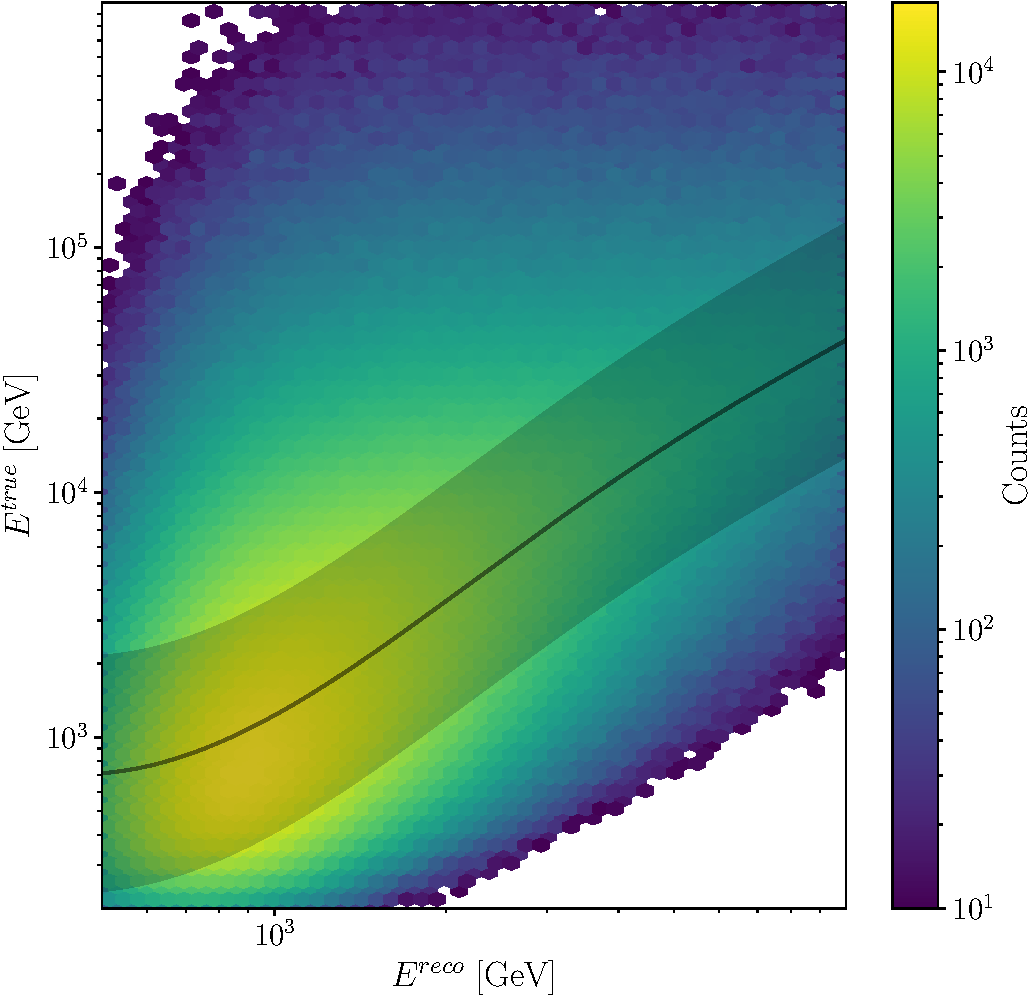
\includegraphics[width=0.7\linewidth]{figures/IC_MC_gpr.pdf}
    \end{center}
    \caption{Relationship between the true and reconstructed muon energy in the IceCube MC sample~\cite{IC2016}.
    The color indicates the frequency of each simulated point.
    Shaded area shows the 99th percentile limits predicted by the regressor trained on this set. It is within this band 
    that then will sample the $\Etrue$ values for each $\Ereco$.}\label{fig:IC_MC_gpr}
 \end{figure}

The latest available data collected and processed by the collaboration contains 305,735 muon track events, collected over eight years~\cite{IC2020}. 
The data has 13 logarithmically spaced bins in $\Ereco \in [500,9976]$ \si{\GeV}, and 20 linear bins in $\zreco \in [-1,0]$. The data is shown in Fig.~\ref{fig:IC_data}.

\begin{figure}[ht]
    \centering
    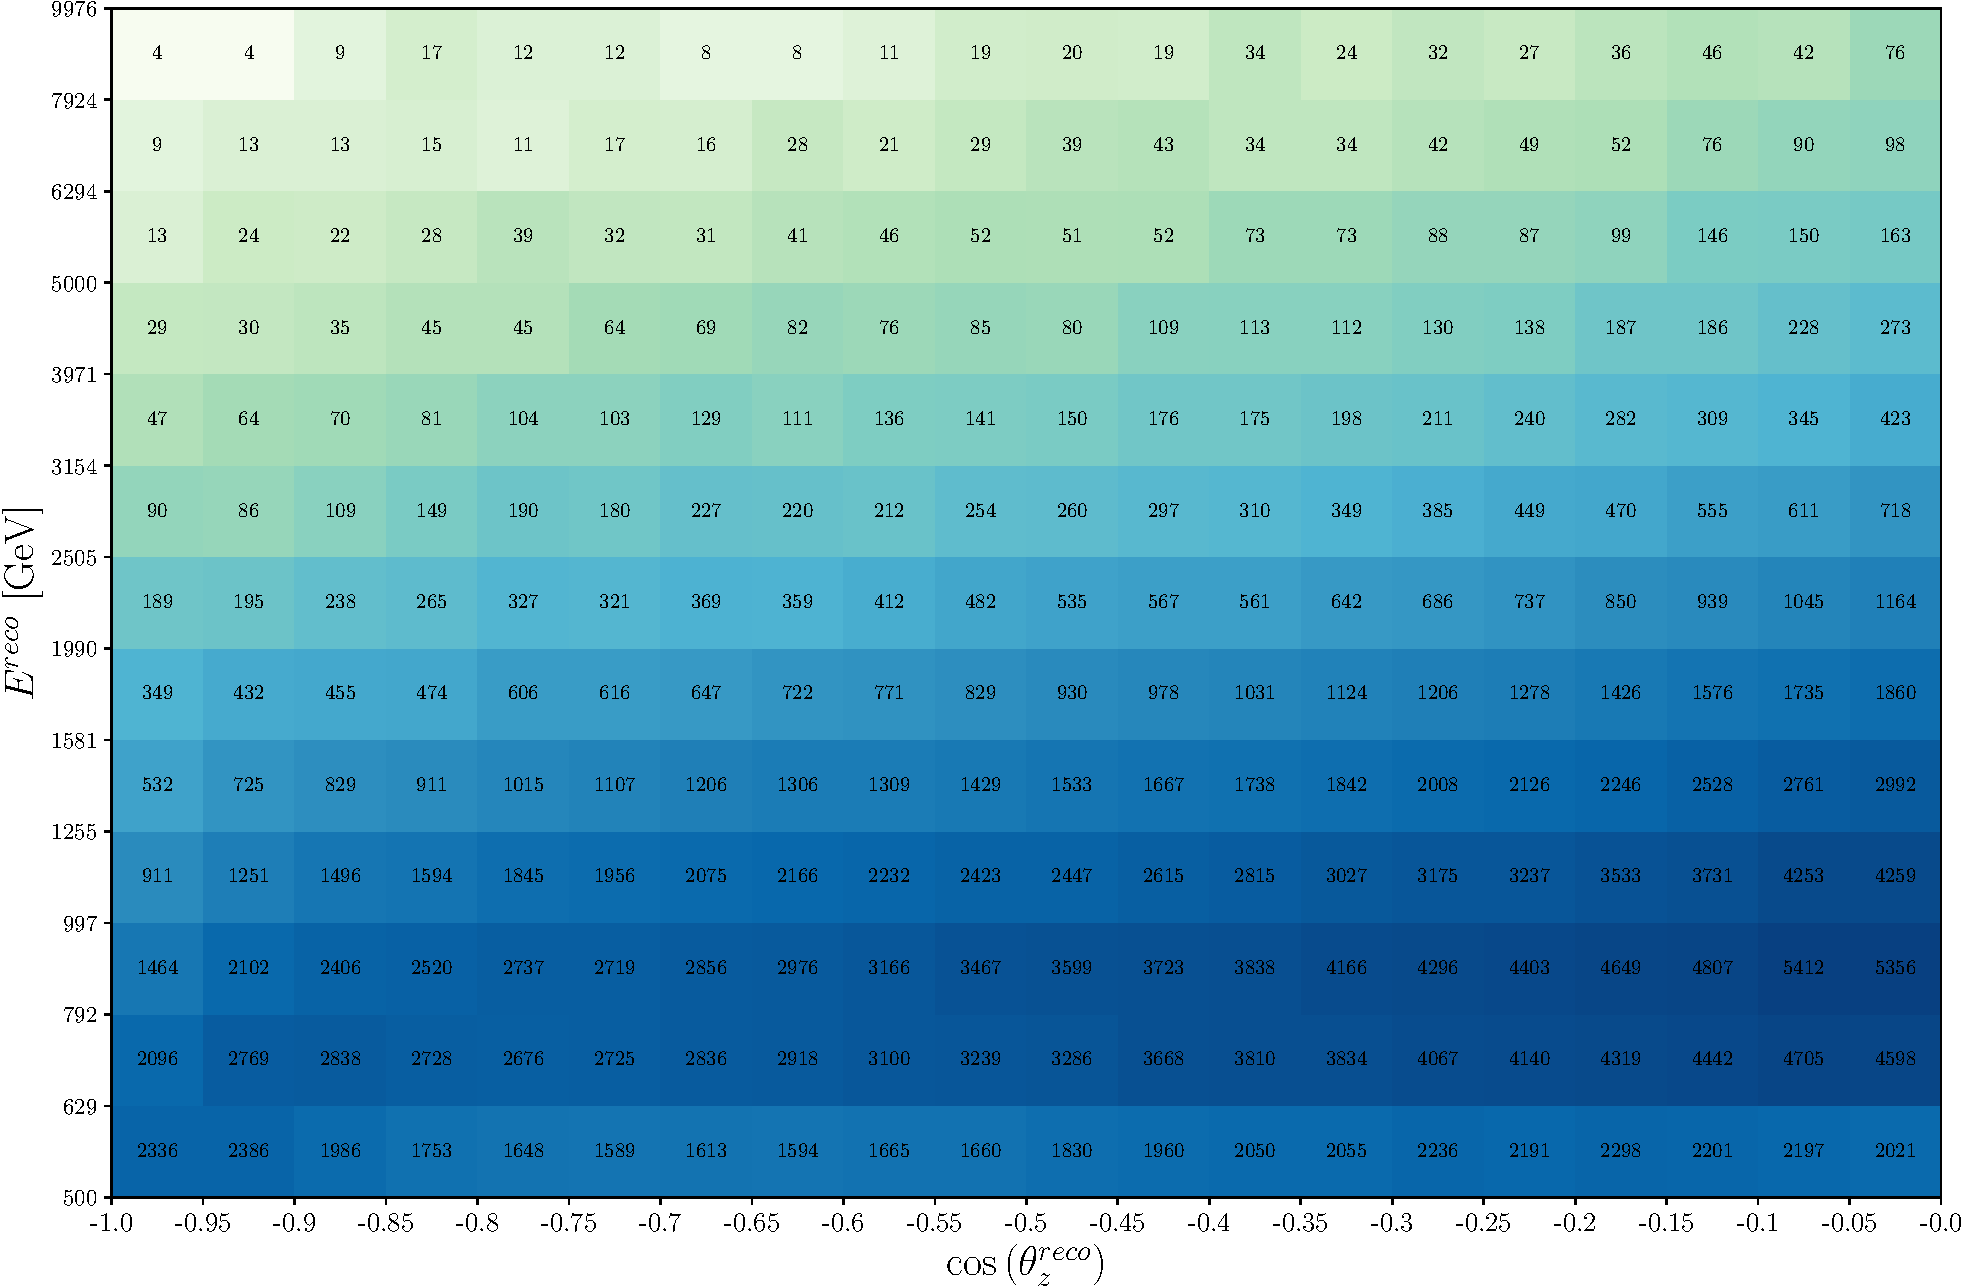
\includegraphics[scale=0.4]{figures/IC_data.pdf}
    \caption{IceCube track events from~\cite{IC2020}, displaying the $E^{-1.7}$ drop-off in event count.}\label{fig:IC_data}
\end{figure}

\subsection*{Monte Carlo normalization}
Independent researchers outside of the IceCube collaboration will not be able to simulate the detector more precisely.
The IceCube Monte Carlo is a complex and proprietary machinery, so our goal in this 
section is merely to come as close as we can to it. After we are confident that 
our code displays the same overall features as the `official', we normalize our results $N_{ij}^\text{sim}$ as 
\begin{align}\label{eq:MC_norm}
    N_{ij} = \frac{N_{ij}^\text{null}}{N_{ij}^\text{MC}} N_{ij}^\text{sim}\,.
\end{align}
For each bin $i,j$, we then obtain a correction factor that contains information that we are unable
to obtain or sufficiently incorporate. One example of such information is the systematic errors of the DOMs.
Recent IceCube data releases do not include such information. Since the systematic errors are affecting the 
event count on a bin-by-bin basis, they can, in theory, drastically modify the binned results. Another example of
an error source that will be remedied by this method is the flux. We are using a fairly simple model of the atmospheric 
flux that excludes atmospheric prompt and astrophysical fluxes. The IceCube collaboration uses several different flux models, which are initialized 
by a parametrization of the cosmic ray flux.\footnote{Included in the cosmic ray models are e.g. the pion to kaon 
ratio, which are often used as a nuisance parameter. By not being able to include this in our error analysis, our method will 
be limited to only consider the overall flux normalization rather than the components that produce the flux in the first place.}

In Fig.~\ref{fig:IC_MC_norm}, we present the IceCube Monte Carlo obtained from their 2020 sterile analysis~\cite{IC2020}, along
with our null hypothesis times a constant factor. 
We used the best-fit values from NuFit~\cite{nufit} with the exception of the CP-violating phase $\delta_\text{CP}$, which was set to $0^\circ$ for simplicity. The values used are
\begin{align}\label{eq:nufitparams}
    \theta_{12} = \SI{33.44}{\degree},\hspace{1em} \theta_{13} = \SI{8.57}{\degree},\hspace{1em} \theta_{23} = \SI{49.2}{\degree}, \hspace{1em} \delta_\text{CP} = 0^\circ\,.
\end{align}

We deemed these shapes to be satisfactory, thus allowing us to multiply Eq.~\ref{eq:ICevents} by the 
correction factors of Eq.~\ref{eq:MC_norm}.
\begin{figure}[ht]
    \begin{centering}
    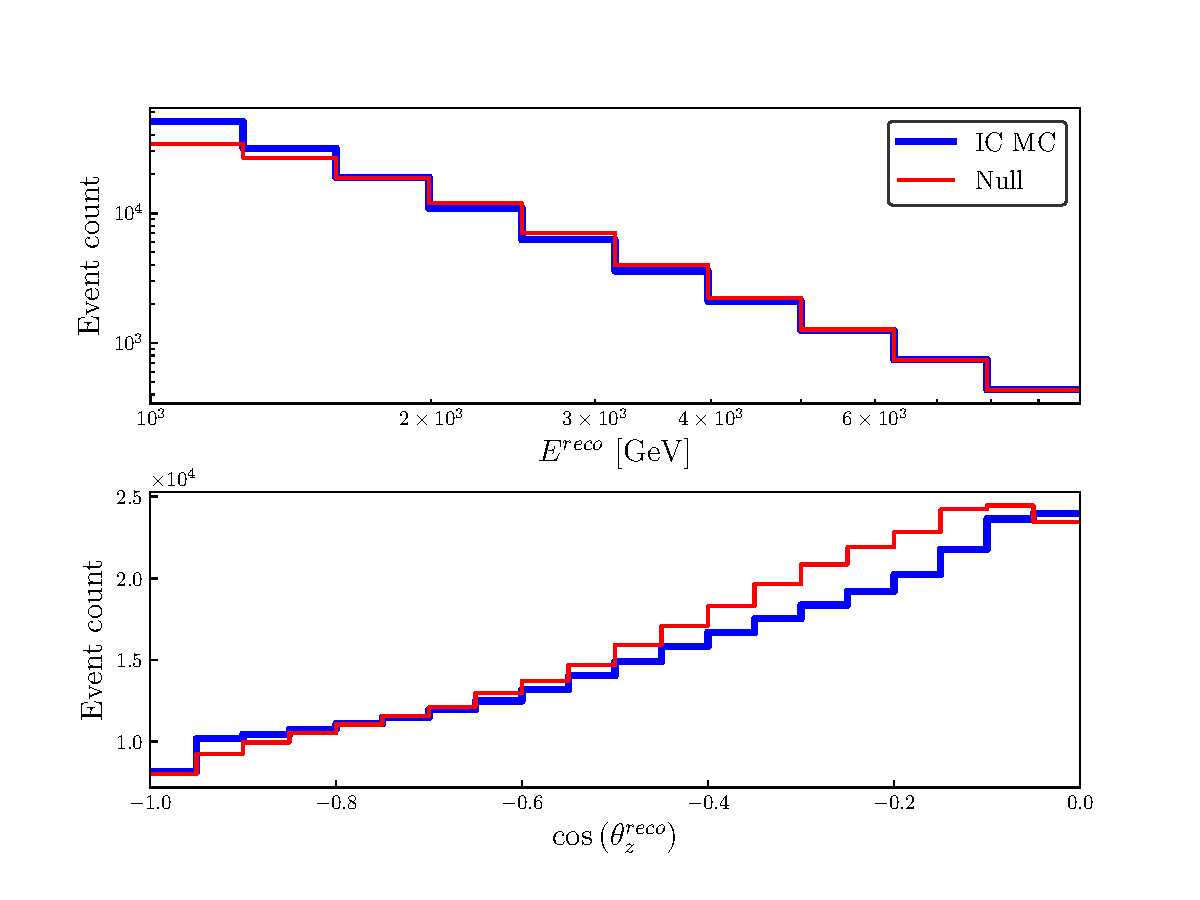
\includegraphics[scale=0.7]{figures/IC_MC_norm.pdf}
    \caption{IceCube Monte Carlo, binned in $\Ereco$ and $\zreco$. We compare this with our simulations shown as `Null' in red in the plots.}\label{fig:IC_MC_norm}
    \end{centering}
\end{figure} 
Thus, we are now able to sufficiently approximate the IceCube Monte Carlo, which makes us able to run simulations based on different physics scenarios.
% \documentclass[draft=True]{thesis}
% \usepackage[margin=0.5in]{geometry}
% \usepackage{graphicx, slashed, siunitx}
% \usepackage[utf8]{inputenc}
% \usepackage{xr-hyper}
% \documentclass[a4paper,10pt,draft]{thesis}
\usepackage{physics,amsmath, amsfonts, siunitx, amssymb, graphicx, slashed,subcaption}
\usepackage[utf8]{inputenc}
\usepackage[margin=1in]{geometry}
\usepackage[hidelinks]{hyperref}
\usepackage{xr-hyper}
\newcommand{\n}[1]{\nu_{#1}}
\newcommand{\na}{\nu_\alpha}
\newcommand{\nb}{\nu_\beta}
\newcommand{\ana}{\bar{\nu}_\alpha}
\newcommand{\an}[1]{\bar{\nu}_{\text{#1}}}
\newcommand{\anb}{\bar{\nu}_\beta}
\renewcommand{\a}{\alpha}
\renewcommand{\b}{\beta}
\newcommand{\ab}{\alpha\beta}


\renewcommand{\ne}{\nu_e}
\newcommand{\nm}{\nu_\mu}
\newcommand{\nt}{\nu_\tau}
\newcommand{\ns}{\nu_s}

\newcommand{\ane}{\bar{\nu}_e}
\newcommand{\anm}{\bar{\nu}_\mu}
\newcommand{\ant}{\bar{\nu}_\tau}
\newcommand{\ans}{\bar{\nu}_s}

\newcommand{\nee}{\nu_e \to \nu_e}
\newcommand{\nem}{\nu_e \to \nu_\mu}
\newcommand{\net}{\nu_e \to \nu_\tau}
\newcommand{\nes}{\nu_e \to \nu_s}

\newcommand{\nme}{\nu_\mu \to \nu_e}
\newcommand{\nmm}{\nu_\mu \to \nu_\mu}
\newcommand{\nmt}{\nu_\mu \to \nu_\tau}
\newcommand{\nms}{\nu_\mu \to \nu_s}



\newcommand{\Pee}{P_{e  e}}
\newcommand{\Pem}{P_{e  \mu}}
\newcommand{\Pet}{P_{e  \tau}}
\newcommand{\Pes}{P_{e  s}}

\newcommand{\Pme}{P_{\mu  e}}
\newcommand{\Pmm}{P_{\mu\mu}}
\newcommand{\Pmt}{P_{\mu  \tau}}
\newcommand{\Pms}{P_{\mu  s}}


\newcommand{\Pte}{P_{P_{\tau e}}}
\newcommand{\Ptm}{P_{\tau  \mu}}
\newcommand{\Ptt}{P_{\tau  \tau}}
\newcommand{\Pts}{P_{\mu  s}}

\newcommand{\Paeae}{P_{\bar{e}  \bar{e}}}
\newcommand{\Paeam}{P_{\bar{e}  \bar{\mu}}}
\newcommand{\Paeat}{P_{\bar{e}  \bar{\tau}}}
\newcommand{\Paeas}{P_{\bar{e}  \bar{s}}}

\newcommand{\Pamae}{P_{\bar{\mu}  \bar{e}}}
\newcommand{\Pamam}{P_{\bar{\mu}  \bar{\mu}}}
\newcommand{\Pamat}{P_{\bar{\mu}  \bar{\tau}}}
\newcommand{\Pamas}{P_{\bar{\mu}  \bar{s}}}


\newcommand{\Patae}{P_{\bar{\tau}  \bar{e}}}
\newcommand{\Patam}{P_{\bar{\tau}  \bar{\mu}}}
\newcommand{\Patat}{P_{\bar{\tau}  \bar{\tau}}}
\newcommand{\Patas}{P_{\bar{\mu}  \bar{s}}}

\renewcommand{\th}[1][]{%
  \theta\ifx\\#1\\\else_\text{#1}\fi
}
\newcommand{\thm}[1][]{%
  \theta^\text{M}\ifx\\#1\\\else_\text{#1}\fi
}
\renewcommand{\t}[1]{\text{{#1}}}
\newcommand{\avg}[1]{\left\langle {#1} \right \rangle}
\newcommand*{\dm}[1][]{%
  \Delta m^2\ifx\\#1\\\else_\text{#1}\fi
}
\newcommand{\zreco}{\cos{(\theta_z^{reco})}}
\newcommand{\ztrue}{\cos{(\theta_z^{true})}}
\newcommand{\z}{\cos{(\theta_z)}}
\newcommand{\Ereco}{E^{reco}}
\newcommand{\Etrue}{E^{true}}
\newcommand{\Aeff}{A^\text{eff}}
\newcommand{\emm}{\epsilon_{\mu\mu}}
\newcommand{\emt}{\epsilon_{\mu\tau}}
\newcommand{\eet}{\epsilon_{e\tau}}
\newcommand{\eem}{\epsilon_{e\mu}}
\newcommand{\ett}{\epsilon_{\tau\tau}}
\newcommand{\ep}{\epsilon^\prime}

% \begin{document}
\section{DeepCore}\label{ch:DCmethod}
In this part, we use the publically available DeepCore data sample~\cite{DC2019data} which is an updated version of what was used by the 
IceCube collaboration in a $\nu_\mu$ disapprearance analysis~\cite{DC2018mudisappearance}.

The detector systematics include ice absorption and scattering, and overall, lateral, and head-on optical efficiencies of the DOMs. 
They are applied as correction factors using the best-fit points from the DeepCore 2019 $\nu_\tau$ appearance 
analysis~\cite{DC2019tauappearance}.

The data include 14901 track-like events and 26001 cascade-like events, both divided into eight 
$ \log_{10}E^{reco} \in [0.75,1.75]$ bins, and eight $\zreco \in [-1,1]$ bins. Each event has a Monte Carlo weight $w_{ijk,\beta}$,
from which we can construct the event count as
\begin{align}\label{eq:MCevents}
    N_{ijk} &= C_{ijk}\sum_{\beta}w_{ijk,\beta} \phi_\beta^\text{det}\,,
\end{align}
where $C_{k\beta}$ is the correction factor from the detector systematic uncertainty and $\phi_\beta^\text{det}$ is defined as Eq.~\ref{eq:propFlux}. We have now substituted the effect of the Gaussian smearing 
by treating the reconstructed and true quantities as a migration matrix. 

The oscillation parameters used on our DeepCore simulations are from the
best-fit in the global analysis in~\cite{nufit}: $\theta_{12} = \SI{33.44}{\degree},\, \theta_{13} = \SI{8.57}{\degree},\, \Delta m^2_{21} =  \SI{7.42}{\electronvolt^2}$, and we 
marginalize over $\dm[31]$ and $\theta_{23}$.

\section{PINGU}
The methodology behind the PINGU simulations is the same as with our DeepCore study~. We use the public MC~\cite{PINGUdata}, which allows us to construct the event count as in Eq.~\ref{eq:MCevents}.
However, since no detector systematics is yet modeled for PINGU, the correction factors $C_{ijk}$ are all unity.
As with the DeepCore data, the PINGU Monte Carlo is divided into eight 
$\log_{10}E^{reco} \in [0.75,1.75]$ bins, and eight $\zreco \in [-1,1]$ bins for both track- and cascade-like events. 
We generate `data' by predicting the event rates at PINGU with the following best-fit parameters from~\cite{nufit}, except for the CP-violating phase which is set to zero for simplicity.

\begin{align}\label{eq:PINGUparams}
    &\Delta m^2_{21} =  \SI{7.42e-5}{\electronvolt^2},\hspace{0.5em} \dm[31] =  \SI{2.517e-3}{\electronvolt^2}, \nonumber \\
    &\theta_{12} = \SI{33.44}{\degree},\hspace{1em} \theta_{13} = \SI{8.57}{\degree},\hspace{1em} \theta_{23} = \SI{49.2}{\degree}, \hspace{1em} \delta_\text{CP} = 0\,.
\end{align}
% \bibliographystyle{nature}
% \bibliography{ref.bib}
% \end{document}
\chapter{Beyond the \texorpdfstring{\boldmath{$3\nu$}}{3 neutrino} Picture}\label{ch:theory}
%\documentclass[a4paper,10pt,draft]{thesis}
\usepackage{physics,amsmath, amsfonts, siunitx, amssymb, graphicx, slashed,subcaption}
\usepackage[utf8]{inputenc}
\usepackage[margin=1in]{geometry}
\usepackage[hidelinks]{hyperref}
\usepackage{xr-hyper}
\newcommand{\n}[1]{\nu_{#1}}
\newcommand{\na}{\nu_\alpha}
\newcommand{\nb}{\nu_\beta}
\newcommand{\ana}{\bar{\nu}_\alpha}
\newcommand{\an}[1]{\bar{\nu}_{\text{#1}}}
\newcommand{\anb}{\bar{\nu}_\beta}
\renewcommand{\a}{\alpha}
\renewcommand{\b}{\beta}
\newcommand{\ab}{\alpha\beta}


\renewcommand{\ne}{\nu_e}
\newcommand{\nm}{\nu_\mu}
\newcommand{\nt}{\nu_\tau}
\newcommand{\ns}{\nu_s}

\newcommand{\ane}{\bar{\nu}_e}
\newcommand{\anm}{\bar{\nu}_\mu}
\newcommand{\ant}{\bar{\nu}_\tau}
\newcommand{\ans}{\bar{\nu}_s}

\newcommand{\nee}{\nu_e \to \nu_e}
\newcommand{\nem}{\nu_e \to \nu_\mu}
\newcommand{\net}{\nu_e \to \nu_\tau}
\newcommand{\nes}{\nu_e \to \nu_s}

\newcommand{\nme}{\nu_\mu \to \nu_e}
\newcommand{\nmm}{\nu_\mu \to \nu_\mu}
\newcommand{\nmt}{\nu_\mu \to \nu_\tau}
\newcommand{\nms}{\nu_\mu \to \nu_s}



\newcommand{\Pee}{P_{e  e}}
\newcommand{\Pem}{P_{e  \mu}}
\newcommand{\Pet}{P_{e  \tau}}
\newcommand{\Pes}{P_{e  s}}

\newcommand{\Pme}{P_{\mu  e}}
\newcommand{\Pmm}{P_{\mu\mu}}
\newcommand{\Pmt}{P_{\mu  \tau}}
\newcommand{\Pms}{P_{\mu  s}}


\newcommand{\Pte}{P_{P_{\tau e}}}
\newcommand{\Ptm}{P_{\tau  \mu}}
\newcommand{\Ptt}{P_{\tau  \tau}}
\newcommand{\Pts}{P_{\mu  s}}

\newcommand{\Paeae}{P_{\bar{e}  \bar{e}}}
\newcommand{\Paeam}{P_{\bar{e}  \bar{\mu}}}
\newcommand{\Paeat}{P_{\bar{e}  \bar{\tau}}}
\newcommand{\Paeas}{P_{\bar{e}  \bar{s}}}

\newcommand{\Pamae}{P_{\bar{\mu}  \bar{e}}}
\newcommand{\Pamam}{P_{\bar{\mu}  \bar{\mu}}}
\newcommand{\Pamat}{P_{\bar{\mu}  \bar{\tau}}}
\newcommand{\Pamas}{P_{\bar{\mu}  \bar{s}}}


\newcommand{\Patae}{P_{\bar{\tau}  \bar{e}}}
\newcommand{\Patam}{P_{\bar{\tau}  \bar{\mu}}}
\newcommand{\Patat}{P_{\bar{\tau}  \bar{\tau}}}
\newcommand{\Patas}{P_{\bar{\mu}  \bar{s}}}

\renewcommand{\th}[1][]{%
  \theta\ifx\\#1\\\else_\text{#1}\fi
}
\newcommand{\thm}[1][]{%
  \theta^\text{M}\ifx\\#1\\\else_\text{#1}\fi
}
\renewcommand{\t}[1]{\text{{#1}}}
\newcommand{\avg}[1]{\left\langle {#1} \right \rangle}
\newcommand*{\dm}[1][]{%
  \Delta m^2\ifx\\#1\\\else_\text{#1}\fi
}
\newcommand{\zreco}{\cos{(\theta_z^{reco})}}
\newcommand{\ztrue}{\cos{(\theta_z^{true})}}
\newcommand{\z}{\cos{(\theta_z)}}
\newcommand{\Ereco}{E^{reco}}
\newcommand{\Etrue}{E^{true}}
\newcommand{\Aeff}{A^\text{eff}}
\newcommand{\emm}{\epsilon_{\mu\mu}}
\newcommand{\emt}{\epsilon_{\mu\tau}}
\newcommand{\eet}{\epsilon_{e\tau}}
\newcommand{\eem}{\epsilon_{e\mu}}
\newcommand{\ett}{\epsilon_{\tau\tau}}
\newcommand{\ep}{\epsilon^\prime}

%\begin{document}
\section{The Sterile State}\label{sec:anomalies}
In 1996, the LSND experiment reported an excess of $\ane$ events from an $\anm$ beam~\cite{lsnd}.  
Nine years later, MiniBooNE not only reproduced the $\ane$ anomaly but observed an excess in the
$\ne$ events too. Together with the so-called reactor and gallium anomalies, these reports suggested 
that the three massive neutrino framework could be amended.
By introducing a fourth heavy mass state $\nu_4$, both appearance and disappearance anomalies could be minimally accommodated.
However, we know from the decay width of the $Z$ boson that it only can interact with three flavor species\footnote{
    Direct measurements of the invisible $Z$ decay yields $N=2.92 \pm 0.05$~\cite{pdg}.
}, 
so this fourth mass state cannot be interacting weakly. In other words, it needs to transform as a
singlet under the gauge symmetry group $SU(2)_L \times U(1)_{Y}$.
We now distinguish between the three original neutrino flavors ($e$, $\mu$, and $\tau$) and the new fourth 
flavor by calling the former \emph{active} neutrinos
and the latter \emph{sterile} due to its non-interacting behavior.

The experiments listed above indicate that the mass-squared difference of the 
sterile neutrino is in the \si{\eV\squared} scale, while the two others
are three and five magnitudes smaller. To remind us of this hierarchy, we write $3+1$, since the sterile state 
proposed is heavier than the active states.


Two neutrino physics parameters probed by CMB lensing observations are the effective number of neutrinos
$N_\text{eff}$, and the sum of neutrino masses $\sum m_i$. 
The 2018 results from the Planck Collaboration in~\cite{planck2018} constrain the parameters to 
\begin{align}
    N_\text{eff} = 2.96^{+0.34}_{-0.33}\,, \quad \sum m_i < \SI{0.12}{\eV} \quad (95\%)\,,
\end{align}
consistent with the Standard Model with oscillations\footnote{Of course, the 
Standard Model \emph{without} neutrino masses dictates $N_\text{eff} = 3$ and $\sum m_i \equiv 0$.} prediction of $N_\text{eff} = 3.045$ degrees~\cite{desalas2016}.
Assuming the Planck data, one thermalized sterile neutrino $(N_\text{eff} = 4)$ is excluded at $6\sigma$. 
Thus, thermalized sterile 
neutrinos are strongly in tension with cosmological observations if one does not consider some special mechanism.
So if a fourth neutrino species is present in nature, it will have ramifications not only on neutrino physics itself, but on
our understanding of the CMB as well.


\subsection{The Hamiltonian}
The inclusion of the sterile state in the Hamiltonian is straightforward. We extend the PMNS matrix
with terms for the mixing between the new flavor $(U_{si})$ and mass $(U_{\a 4})$ eigenstates:
\begin{align}
    U_{4gen} =
    \begin{pmatrix}
    U_{e1} & U_{e2} & U_{e3} & U_{e4} \\
    U_{\mu1} & U_{\mu2} & U_{\mu3} & U_{\mu4} \\
    U_{\tau1} & U_{\tau2} & U_{\tau3} & U_{\tau4} \\
    U_{s1} & U_{s2} & U_{s3} & U_{s4}
    \end{pmatrix}\,,
\end{align}
where a common parametrization of this new mixing matrix is 
\begin{align}\label{eq:U4gen_param}
    U_{4gen} = R_{34}R_{24}R_{14}U_{3gen}\,.
\end{align}
This parametrization does not affect the physics, but determines the structure of the mixing angles.

The mass matrix extends analogously:
\begin{align}\label{eq:dm4gen}
    M^2_{4gen} =
    \begin{pmatrix}
        0 & 0 & 0 & 0\\
        0 & \dm_{21} & 0  & 0 \\
        0 & 0 & \dm_{31} & 0 \\
        0 & 0 & 0 & \dm_{41} \\
    \end{pmatrix}\,.
\end{align}

Now, the interaction with matter requires a careful reconsideration of the matter potential. We start off with the unaltered potential matrix from Eq.~\ref{eq:V_matrix}. 
Just as with the PMNS matrix, we extend this to $4\times4$:
\begin{align}\label{eq:Vsterile1}
    \begin{pmatrix}
        V_{CC} + V_{NC} & 0 & 0 & 0 \\
        0 &V_{NC} & 0 & 0 \\
        0 & 0 & V_{NC} & 0 \\
        0 & 0 & 0 & 0 
    \end{pmatrix}\,.
\end{align}
Now we need to include the terms that describes the matter potential felt by the sterile flavor state. Recalling our discussion above, we remind ourselves that the sterile neutrino by definition
does not participate in any interaction\footnote{The exception to this is of course gravity. The sterile neutrino is not massless.}. Thus, all potential terms involving the sterile state are zero. 
In other words, the potential matrix in Eq.~\ref{eq:Vsterile1} is complete, save for the usual subtraction by a constant times the identity matrix:

\begin{align}\label{eq:Vsterile}
    V_{4gen} &=
    \begin{pmatrix}
        V_{CC} + V_{NC} & 0 & 0 & 0 \\
        0 &V_{NC} & 0 & 0 \\
        0 & 0 & V_{NC} & 0 \\
        0 & 0 & 0 & 0 
    \end{pmatrix} - V_{NC}\begin{pmatrix}
        1 & 0 & 0 & 0 \\
        0 &1 & 0 & 0 \\
        0 & 0 & 1 & 0 \\
        0 & 0 & 0 & 1 
    \end{pmatrix} \nonumber \\
    &= \sqrt{2}G_F\begin{pmatrix}
        N_e & 0 & 0 & 0 \\
        0 &0 & 0 & 0 \\
        0 & 0 & 0 & 0 \\
        0 & 0 & 0 & -N_n/2
    \end{pmatrix} \nonumber \\
    &=\sqrt{2}G_F N_e\begin{pmatrix}
        1 & 0 & 0 & 0 \\
        0 &0 & 0 & 0 \\
        0 & 0 & 0 & 0 \\
        0 & 0 & 0 & -1/2
    \end{pmatrix}\,.
\end{align}
where we have assumed electrical neutrality in the last step, yielding $N_e = N_n$.
Thus, the final Hamiltonian with a fourth sterile neutrino is 
\begin{align}\label{eq:H_4gen}
    H_{4gen} &= \frac{1}{2E}\left[U \begin{pmatrix}
            0 & 0 & 0 & 0\\
            0 & \dm_{21} & 0  & 0 \\
            0 & 0 & \dm_{31} & 0 \\
            0 & 0 & 0 & \dm_{41} \\
        \end{pmatrix} U^\dagger\right] + \sqrt{2}G_F N_e 
        \begin{pmatrix}
            1 & 0 & 0 & 0 \\
            0 & 0 & 0 & 0 \\
            0 & 0 & 0 & 0 \\
            0 & 0 & 0 & -1/2
        \end{pmatrix}\,. 
\end{align}

Now, looking at Eqs.~\ref{eq:U4gen_param} and~\ref{eq:dm4gen}, we see that we have introduced four new parameters: $\dm[41]$, $\theta_{14}$
, $\theta_{24}$, $\theta_{34}$. In our analysis, we reduce the number of parameters by only considering $\dm[41]$ and $\theta_{24}$, which are 
the most important for the $\nm$ oscillations. 

\subsection{The Probability Effect of a Sterile Neutrino}
Since the new, sterile, neutrino does not interact weakly, how do we know if it's there? If the sterile mixing angle $\theta_{i4}$ is non-zero, 
we allow the sterile mass state to mix with the active state $i$. The most interesting case is when $\theta_{24} \neq 0$, 
which for $\dm[41] \sim \si{\eV \squared}$ gives rise to a resonant disappearance in the for $P_{\bar{\mu}\bar{\mu}}$, shown in Fig.~\ref{fig:sterile_resonance}.

\begin{figure}
    \centering
        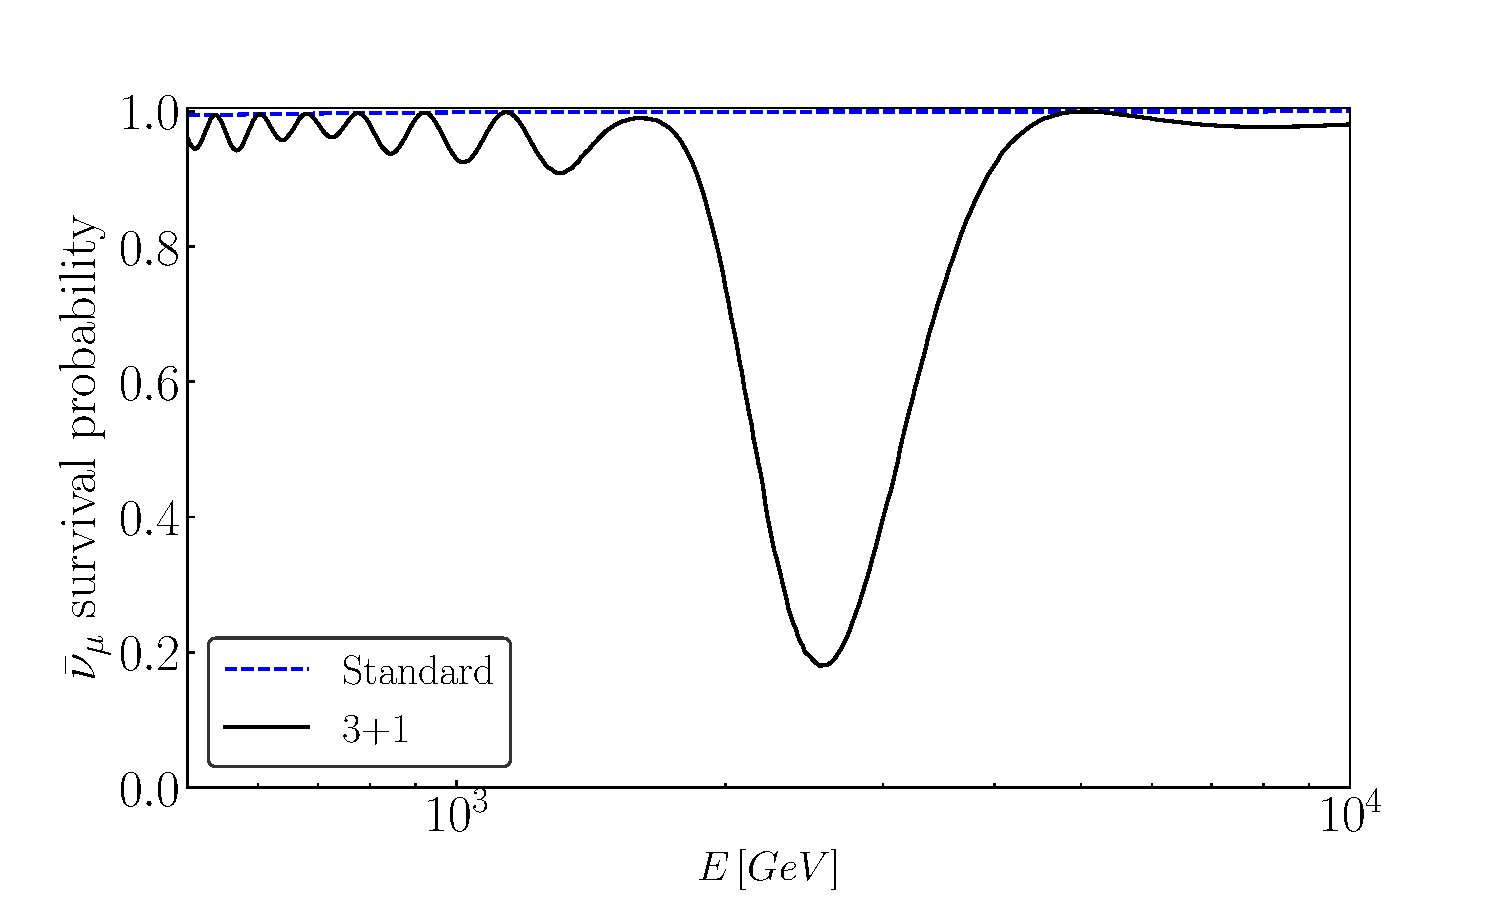
\includegraphics[width=1\linewidth]{figures/sterile_resonance.pdf}
        \caption{Comparing the standard 3+0 hypothesis to the
        3+1 hypothesis assuming $\dm[41] = \SI{1}{\eV \squared}$ and $\theta_{24} = 0.04$.
        The former, shown as a blue dashed line, shows no $\anm$ disappearance.
        The latter, shown as a black solid line, predicts a resonant $\anm$ disappearance at \SI{2.6}{\TeV}.
        The standard oscillation parameters are taken from NuFit~\cite{nufit}, and the 
        neutrino has traversed the entire Earth diameter.}\label{fig:sterile_resonance}
    \end{figure}
    \begin{figure}
        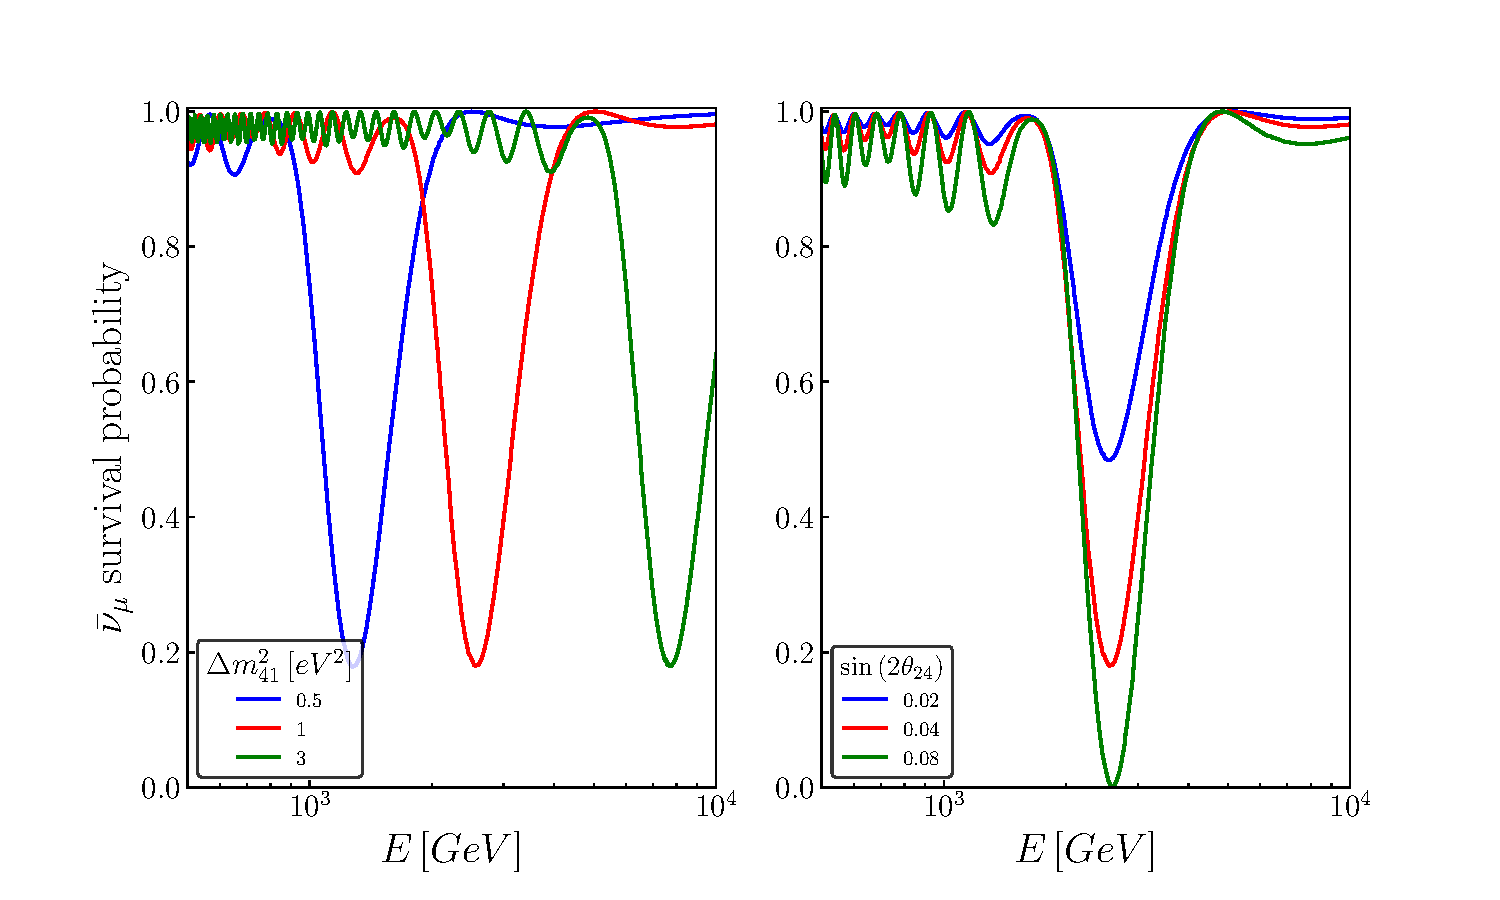
\includegraphics[width=1\linewidth]{figures/resonance_shift.pdf}
        \caption{Shifting and amplification of the resonance by altering $\dm[41]$ and $\theta_{24}$, respectively.
        Left panel has a fixed value of $\theta_[24] = 0.04$ while varying $\dm[41]$ from 0.5 to 3 \si{\TeV^2}.
        Right panel has a fixed value of $\dm[41] = \SI{1}{\TeV^2}$ while varying $\theta_[24]$ from 0.02 to 0.08.
        Standard oscillation parameters are taken from NuFit~\cite{nufit}, and shown in Eq.~\ref{eq:PINGUparams}.}\label{fig:resonance_shift}
\end{figure}
So for a \si{\eV^2}-scale sterile neutrino and a non-zero $\theta_{24}$, we expect a \si{\TeV} $\anm$ disappearance.
The resonance dip is affected by the value of $\dm[41]$ and $\theta_{24}$ as shown in Fig.~\ref{fig:resonance_shift}.
We see how the value of $\dm[41]$ shifts the resonance peak, while the mixing angle amplifies it. 
In the $3+0$ scenario, $\Pamam = 1$ in this range. Thus, if we are able to see a $\anm$ disappearance in the \si{\TeV} region,
we are in a good position to argue for an \si{\eV^2}-scale $\dm[41]$.  

Keeping in mind that the event count from Eq.~\ref{eq:ICevents} scales as $E^{-1.7}$,
signals at higher energies will be more difficult to detect. Since higher values of $\dm[41]$ shifts the $\Pamam$ resonance peak to higher 
energies, high $\dm[41]$ values will be harder to rule out because the event count is already lower, as compared to energies 
at single-digit \si{\TeV} values. There is then a range of parameters, in which our detector will 
be able to distinguish between the two hypotheses. Using the two-neutrino approximation\footnote{In this approximation, we only consider mixing between $\nm$ and $\ns$, essentially a `1+1' picture.}, 
we can rewrite the expression for MSW resonance from Eq.~\ref{eq:MSW} as 
\begin{align}
    E^* = \frac{\dm[41] \cos{2\theta_{24}}}{2\sqrt{2} G_F N_e}\,,
\end{align}
which for $\dm[41] = \SI{1}{\TeV^2}$ and $\theta_{24} = 0.04$, gives us a resonance at $E^* = \SI{2.58}{\TeV}$, matching the $3+1$ simulation shown in
Fig.~\ref{fig:sterile_resonance}. From the two-neutrino picture, 
we see that the resonance peak in the $\anm$ channel scales linearly with $\dm[41]$, while the mixing angle dependence 
shows up as $\cos{2\theta_{24}}$, which is between 0.987 and 0.999 for the $\theta_[24]$ values considered in Fig.~\ref{fig:resonance_shift}.
Since our $\theta_{24}$ values considered are so low, the location of the resonance peak is essentially only dependent on the value of $\dm[41]$.
Thus, we expect a more stringent constraint of low values of $\dm[41]$, regardless of the value of $\theta_{24}$.

We also note that lower values of $\theta_{24}$ suppresses the 3+1 signal, making it closer to the $3+0$ hypothesis. 
Regardless of the value of $\dm[41]$, the $3+1$ hypothesis asymptotically converges to the $3+0$ hypothesis as $\theta_{24} \to 0$.
\section{Non-Standard Interactions}\label{sec:nsiTheory}
We have no reason to believe that the Standard Model 
gauge group is the complete picture. We have already seen how the failure of the Standard Model to predict neutrino masses and 
oscillations forces us to amend it. 
Just as the electroweak theory $SU(2)_L \times U(1)_Y$ is 
spontaneously broken to $U(1)_{EM}$, a higher order theory at a different energy scale with completely different
properties might undergo a similar spontaneous symmetry break at high energies, 
producing at lower energies the Standard Model that we know. In fact, 
just as the fermion masses originate from the electroweak symmetry breaking, the neutrino masses might be generated from 
another broken symmetry resulting in the Standard Model gauge group.
In this sense, the Standard Model might be considered 
an effective low energy theory, which is yields impressive results in some areas, but failing in others. 

Compared to other fermions, the lightness of neutrino masses\footnote{The extreme lightness might be explained by a mass generation at a higher order theory.} along with their sparse SM interactions might 
indicate that these particles provide the best starting point for us to probe new physics, in which exotic neutrino interactions might occur~\cite{gavela2009}. We call these interactions non-standard interactions (NSI) in order to 
distinguish them from the `standard' interactions of the Standard Model.
 
Following the approach of the Standard Model that the group generators uniquely determine the gauge bosons, a different gauge
theory will have different interactions than those we presently know. These new interactions can be parametrized as model-independent four-fermion effective operators \cite{salvadoNSI,nsiFarzan}.
Following the discussion in~\cite{tommyNSI}, we see that the NSI parameters $\epsilon$ resulting from six-dimensional operators have the scale
\begin{align}
    \epsilon \propto \frac{m_W^2}{m_{\epsilon}^2} \sim \frac{10^{-2}}{m_\epsilon^2}\,
\end{align} 
in \si{\TeV}, so the new interactions generated at a mass scale of $m_\epsilon = \SI{1}{TeV}$ will produce parameters in the order of $10^{-2}$, 
two magnitudes below the standard matter effect. Thus, if we assume the new interactions to arise from a higher-energy theory above electroweak scale, 
we then predict that the parameters contribute with at most a factor of $10^{-2}$ to the standard matter effect, decreasing quadratically.


\subsection{Non-Standard Effects on Neutrino Matter Interactions}
Up until now, we have only considered weak neutrino interactions with electrons, protons, and neutrons.
We can phenomenologically allow these interactions to include the up and down quarks which are present 
in the Earth as the fundamental components of neutrons and protons, as seen in the Lagrangians
\begin{align*}
    \mathcal{L}_{\mathrm{CC}} &= -2 \sqrt{2} G_{F} \epsilon_{\alpha \beta}^{f f^{\prime} X}\left(\bar{\nu}_{\alpha} \gamma^{\mu} P_{L} \ell_{\beta}\right)\left(\bar{f}^{\prime} \gamma_{\mu} P_{X} f\right) \\
    \mathcal{L}_{\mathrm{NC}} &= -2 \sqrt{2} G_{F} \epsilon_{\alpha \beta}^{f X}\left(\bar{\nu}_{\alpha} \gamma^{\mu} P_{L} \nu_{\beta}\right)\left(\bar{f} \gamma_{\mu} P_{X} f\right)\,,
\end{align*}
where CC denotes the charged current interaction with the matter field $f\neq f^\prime \in \{u,d\}$, and NC denotes the neutral current interaction with 
$f \in \{e,u,d\}$. The CC NSI effect affects neutrino production and detection, and will not be considered further. NC NSI affect the matter potential, 
and is thus of interest to us.

We have no independent sensitivity for the neither chirality nor flavor type of $\epsilon^X$, so we sum over these and study the effective matter NSI parameter
 $\epsilon_{\ab}$:
\begin{align}
    \epsilon_{\ab} = \sum_{X \in \{L,R\}} \sum_{f \in \{e,u,d\}} \frac{N_f}{N_e} \epsilon^{fX}_{\ab}\,.
\end{align}
Our matter study will be wholly confined to the interior of the Earth, where we assume electrical neutrality and equal distribution of neutrons and protons, 
we get $N_u/N_e \simeq N_d/N_e \simeq 3$. Also we assume the components $\epsilon_{\a\b}$ to be real. Thus,
\begin{align}
    \epsilon_{\ab} =  \sum_X \epsilon_{\ab}^{eX} + 3(\epsilon_{\ab}^{uX} + \epsilon_{\ab}^{dX})
\end{align}
Now, $\epsilon_{\ab}$ enters the Hamiltonian as entries of a potential-like matrix. In Eq.~\ref{eq:NSIH}, $A_{CC}\text{diag}(1,0,0)$ is our 
familiar matter potential from the Standard Model. There is also our new term, $A_{CC} \epsilon$, which contains the components $\epsilon_{\a\b}$:
\begin{align}\label{eq:NSIH}
    H &= \frac{1}{2E} \left[UM^2U^\dagger + A_{CC}\,\text{diag}(1,0,0) + A_{CC}\, \epsilon \right] \nonumber \\
      &= \frac{1}{2E} \left[UM^2U^\dagger + A_{CC}
      \begin{pmatrix}
          1 + \epsilon_{ee} & \epsilon_{e\mu} & \epsilon_{e\tau}  \\
          \epsilon_{\mu e} & \epsilon_{\mu\mu} & \epsilon_{\mu\tau}  \\
          \epsilon_{\tau e} & \epsilon_{\tau\mu} & \epsilon_{\tau\tau}
      \end{pmatrix} \right]\,.
\end{align} 
In the limit $\epsilon_{\ab} \to 0$, we recover the standard interaction Hamiltonian from Eq.~\ref{eq:H_3gen}.
We can draw several conclusions from this form of the Hamiltonian. Any nonzero off-diagonal element $\epsilon_{\ab}, \a \neq \b$ contribute
to neutrino mixing, just as the off-diagonal elements of $U$ does in the SM. Moreover, since the SM potential has the same order in $A_{CC}$ as the NSIs, 
any $\epsilon_{\ab} \sim 1$ will make the new matter effect be the same order as the SM effect.

We have two more modifications to the matrix $\epsilon$. First, all terms of the Hamiltonian must of course be Hermitian, thus
\begin{align}
    \begin{pmatrix}
        \epsilon_{ee} & \epsilon_{e\mu} & \epsilon_{e\tau}  \\
        \epsilon_{\mu e} & \epsilon_{\mu\mu} & \epsilon_{\mu\tau}  \\
        \epsilon_{\tau e} & \epsilon_{\tau\mu} & \epsilon_{\tau\tau}
    \end{pmatrix} =
    \begin{pmatrix}
        \epsilon_{ee} & \epsilon_{e\mu} & \epsilon_{e\tau}  \\
        \epsilon_{e \mu} & \epsilon_{\mu\mu} & \epsilon_{\mu\tau}  \\
        \epsilon_{e\tau} & \epsilon_{\mu\tau} & \epsilon_{\tau\tau}
    \end{pmatrix}\,.
\end{align}
Now we have reduced the possible number of NSI parameters from 9 down to 6. 

By combining oscillation data and neutrino-nucleon scattering at the COHERENT experiment, 90 \% CL ranges of some of 
the NSI parameters were constrained in~\cite{coherent} to
\begin{align}\label{eq:coherentbounds}
    -0.090 < &\,\ett < 0.38 \nonumber \\
    -0.01 < &\,\emt < 0.009 \nonumber \\
    -0.073 < &\,\eem < 0.044 \nonumber \\
    -0.15 < &\,\eet < 0.13\,.
\end{align}


\subsection{IceCube Signal}
In our analysis of IceCube, we are constrained to muon track events. Thus, we are not able to test any theory which does not modify $P_{\a \mu}$. Moreover,
the IceCube data is available in the range \SI{500}{\GeV} to \SI{10}{\TeV} range, where any rapid oscillations have averaged out.

Since all standard matter potentials are diagonal, 
the elements $\epsilon_{\a\b},\, \a = \b$ will directly adjust the matter potential felt 
by flavor $\a$. The off-diagonal terms have a more interesting theoretical implication as they open up matter interactions across flavors. Remember, in the Standard model,
we are restricted to weak interactions that conserve lepton flavor. However, an off-diagonal NSI parameter allows flavor transitions during matter interactions. Thus,
the off-diagonal elements constitute new sources of flavor violation.
Moreover, $\epsilon_{\a\b}$ modifies the $\nu_\a \to \nu_\b$ transition independently
of the mixing matrix. Thus, we are not confined to the parameters of the mixing matrix: now we have introduced the 
possibility of additional interactions that can cause the flavor change. Moreover, since we have 6 NSI parameters, and the PMNS
matrix is parametrized with only 3 parameters, we have more degrees of freedom when adjusting the probabilities using the NSI matrix. Each term in the PMNS matrix consists of at least
two of the three mixing angles, making the individual angles more inter-dependent than the NSI parameters, since combinations of them must satisfy the constraints of the matrix elements.

As discussed in Eq.~\ref{eq:Uvalues}, the atmospheric $\nm \to \nt$ transition will be the most abundant, making $\emt$, $\emm$, $\ett$ the most suitable
NSI parameters to constrain from muon events. As we will see, $\eem$ is also a candidate, albeit a weaker one. 

In Fig.~\ref{fig:emt_ett_probs}, we see how the introduction of $\emt = 0.02$ alters the $\nm$ and $\anm$ survival probabilities
for neutrinos that traverse the entire Earth diameter (i.e. $\ztrue = -1$). $\emt$ does not dramatically change neither
amplitude nor frequency of the probabilities. Instead, it seems to stretch or compress the oscillations. Since the 
only difference between the way neutrinos and antineutrinos interact with matter is the sign of the potential, the probability for
$\nm$ with positive $\epsilon_{\a\b}$ is identical to the probability for $\anm$ with negative $\epsilon_{\a\b}$. Thus, the dashed line 
in the right panel not only shows the survival probability for $\anm$ with $\emt=0.02$, but also the survival probability for $\nm$ with $\emt=-0.02$.
Hence, we note that $\emt > 0$ stretches (compresses) $\Pmm$ for neutrinos (antineutrinos), while $\emt < 0$ compresses (stretches) $\Pmm$ for neutrinos (antineutrinos).

The value of $\ett$ affects neither $\Pmm$ nor $\Pamam$, in the IceCube region above \SI{500}{\GeV}. Hence, we will not be able
to say anything about $\ett$ in our IceCube study.  Comparing the probabilities in Fig.~\ref{fig:emt_ett_probs} with $\ett = 0.05$ with the ones for $\emt = 0.02$ in Fig.~\ref{fig:emt_ett_probs},
we see that even though we let $\ett$ take 2.5 times the value of $\emt$, its effect on $\Pmm$ is smaller. The weakening of the $\Pamam$ resonance will be visible in DeepCore, but we should expect a less stringent 
constraint due to the weakness of the effect compared to $\emt$. 

Thus, we will use IceCube to constrain $\emt$ only.


Moving on to $\eem$ and Fig.~\ref{fig:eem_eet_probs}, we see that both probabilities has shifted downwards for $\Etrue > \SI{500}{\GeV}$.
In Fig.~\ref{fig:eem_eet_probs}, we see that the muon channel remains largely unaffected of the value of $\eet$ as we expected. The exception of this lies 
in the DeepCore region of rapid oscillations, where mixing is more violent. 
\begin{figure}
    \begin{center}
        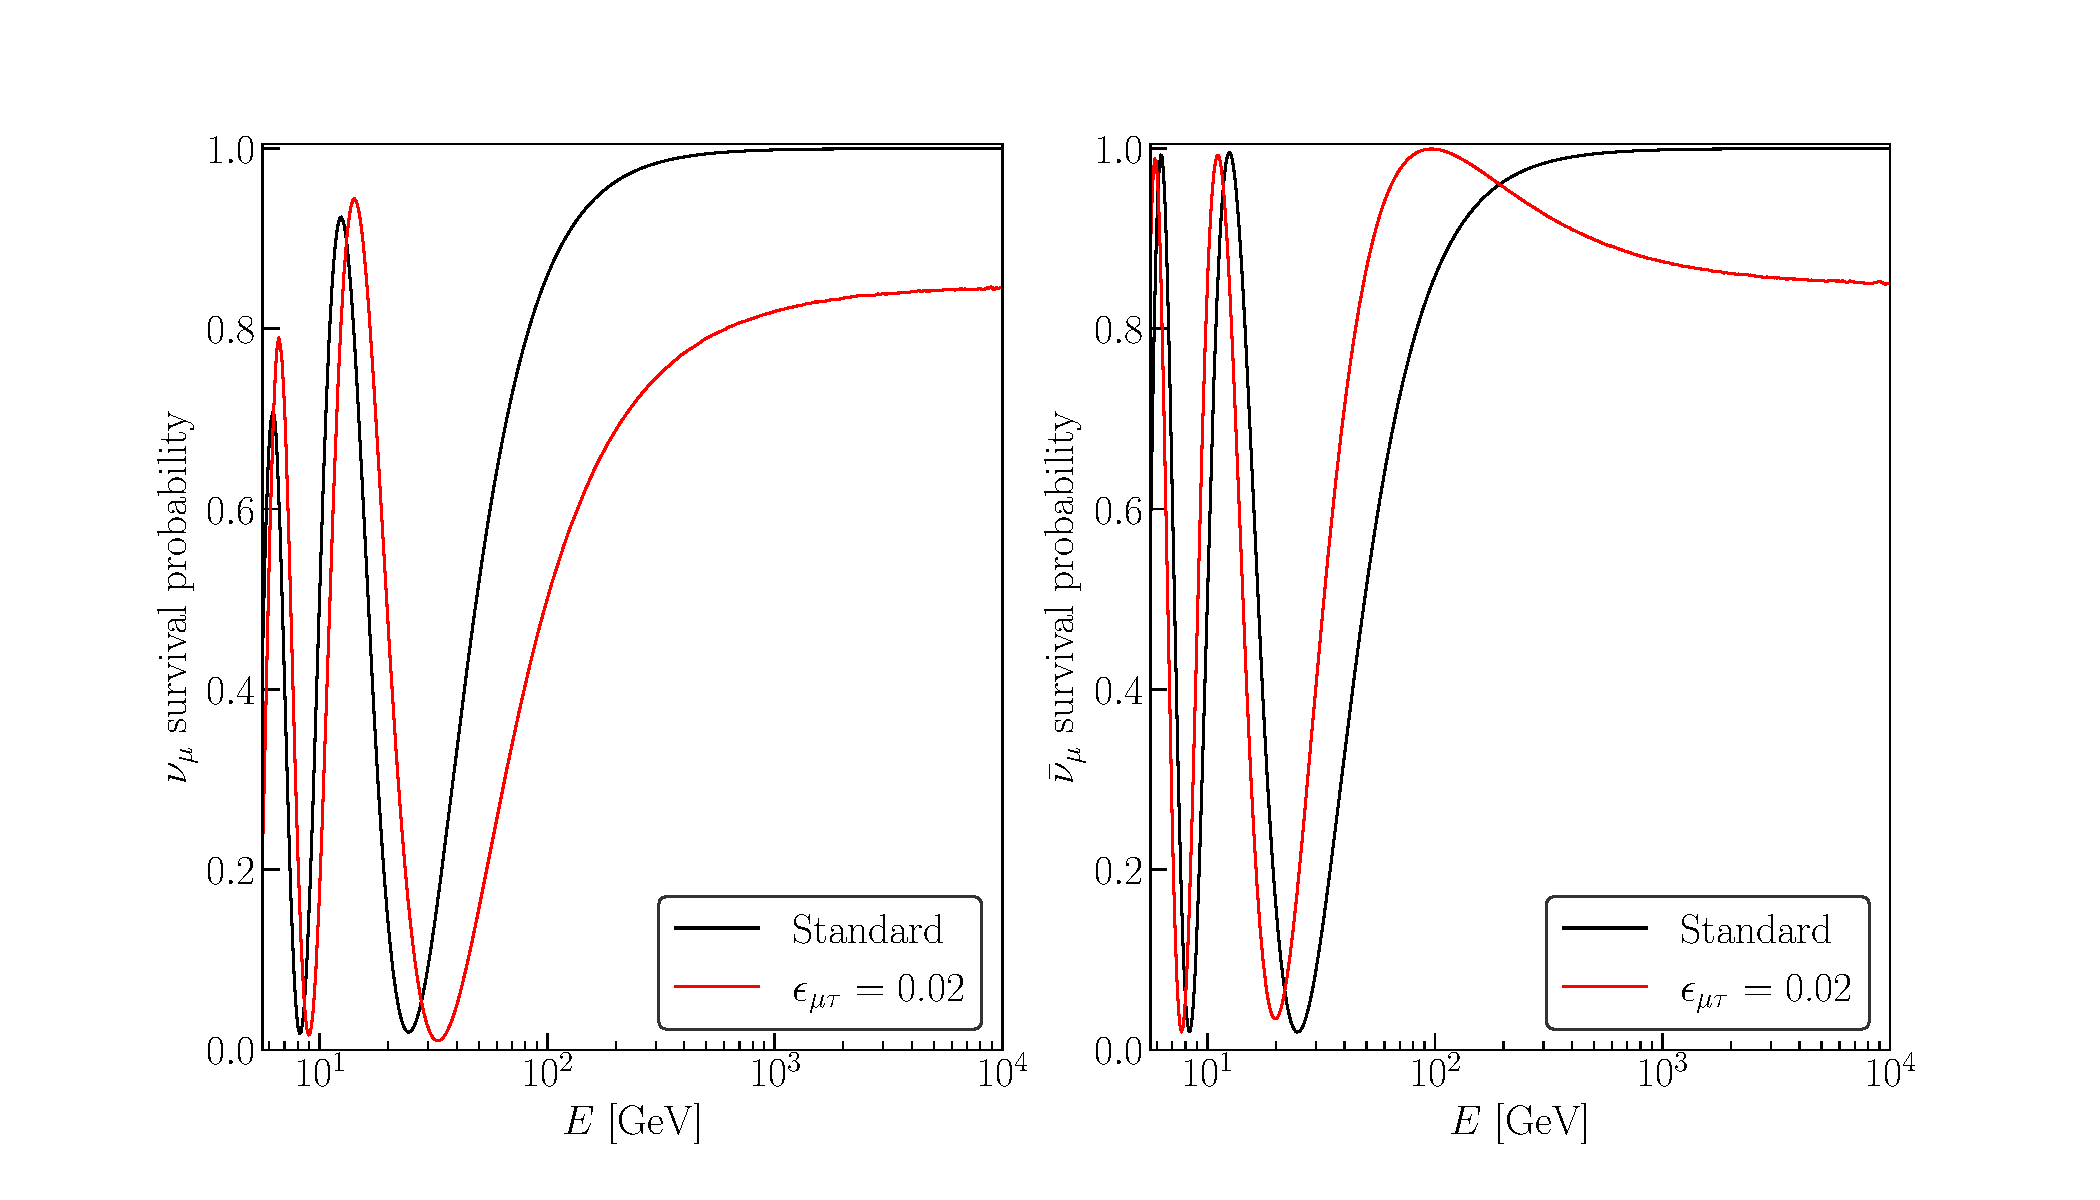
\includegraphics[width=0.99\textwidth]{figures/Pmm_emt_probs.pdf}
        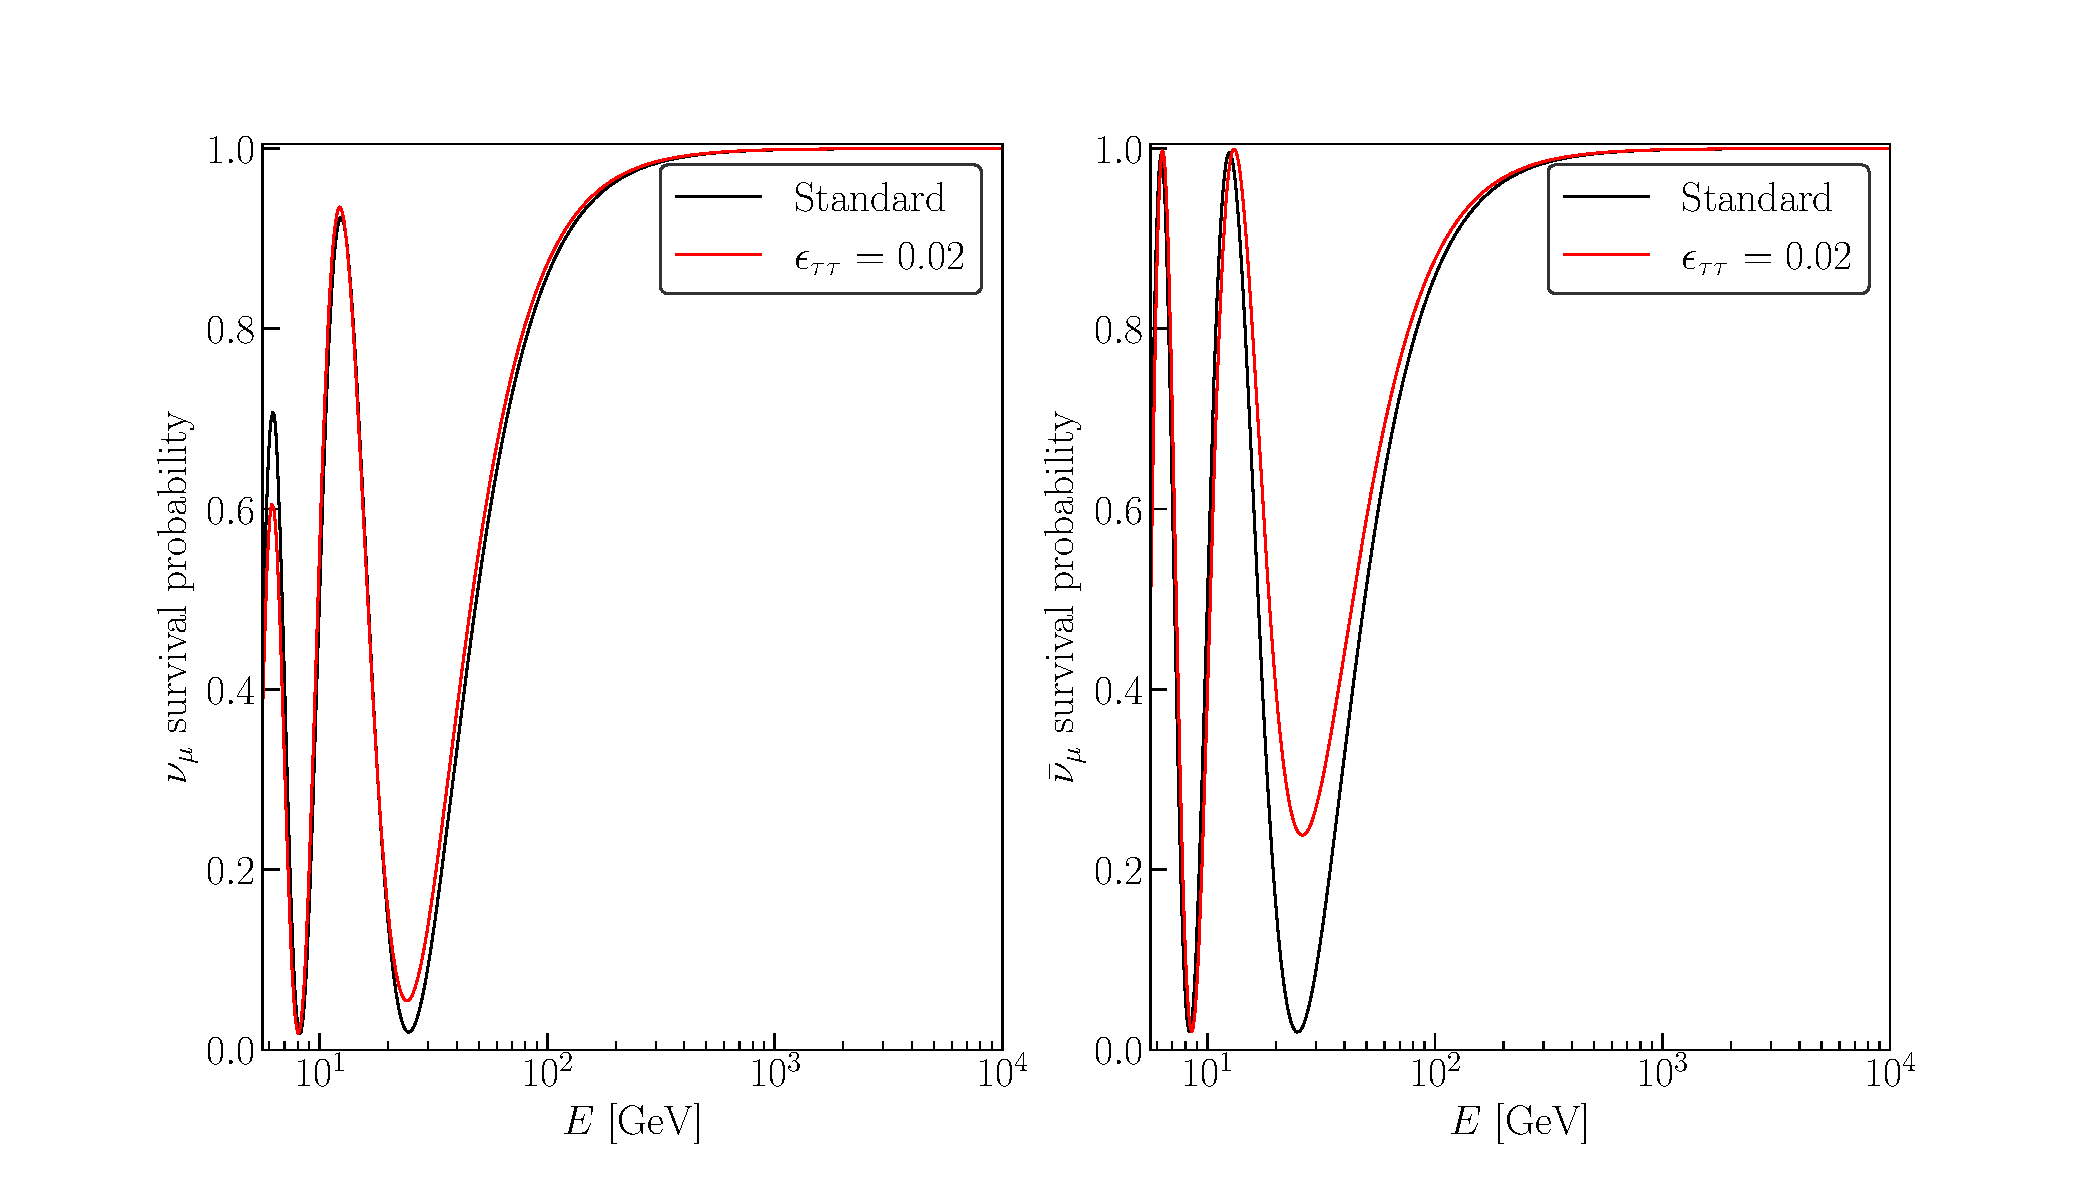
\includegraphics[width=0.99\textwidth]{figures/Pmm_ett_probs.pdf}
        \caption{\emph{Top panel:} Muon neutrino and antineutrino survival probabilities for
        $\ztrue = -1$ when $\emt = 0.02$. All other NSI parameters are fixed to zero. In the \si{\GeV} range, $\emt$ shifts the oscillations to the right for $\nm$, and to the left for $\anm$. At \si{\TeV} energies, both probabilities simply get shifted down, resulting in a net reduction of track events.
        \emph{Bottom panel:} Muon neutrino and antineutrino survival probabilities for
        $\ztrue = -1$ when $\ett = 0.05$. All other NSI parameters are fixed to zero. $\ett$ does not affect the probabilities above \SI{100}{\GeV} and this parameter is thus unable to be constrained by tracks in IceCube in our study. However, the dampening of the $\anm$ survival probability will be visible to DeepCore and PINGU, since it occurs within their energy ranges.}
        \label{fig:emt_ett_probs}
    \end{center}
\end{figure}


\begin{figure}
    \begin{center}
        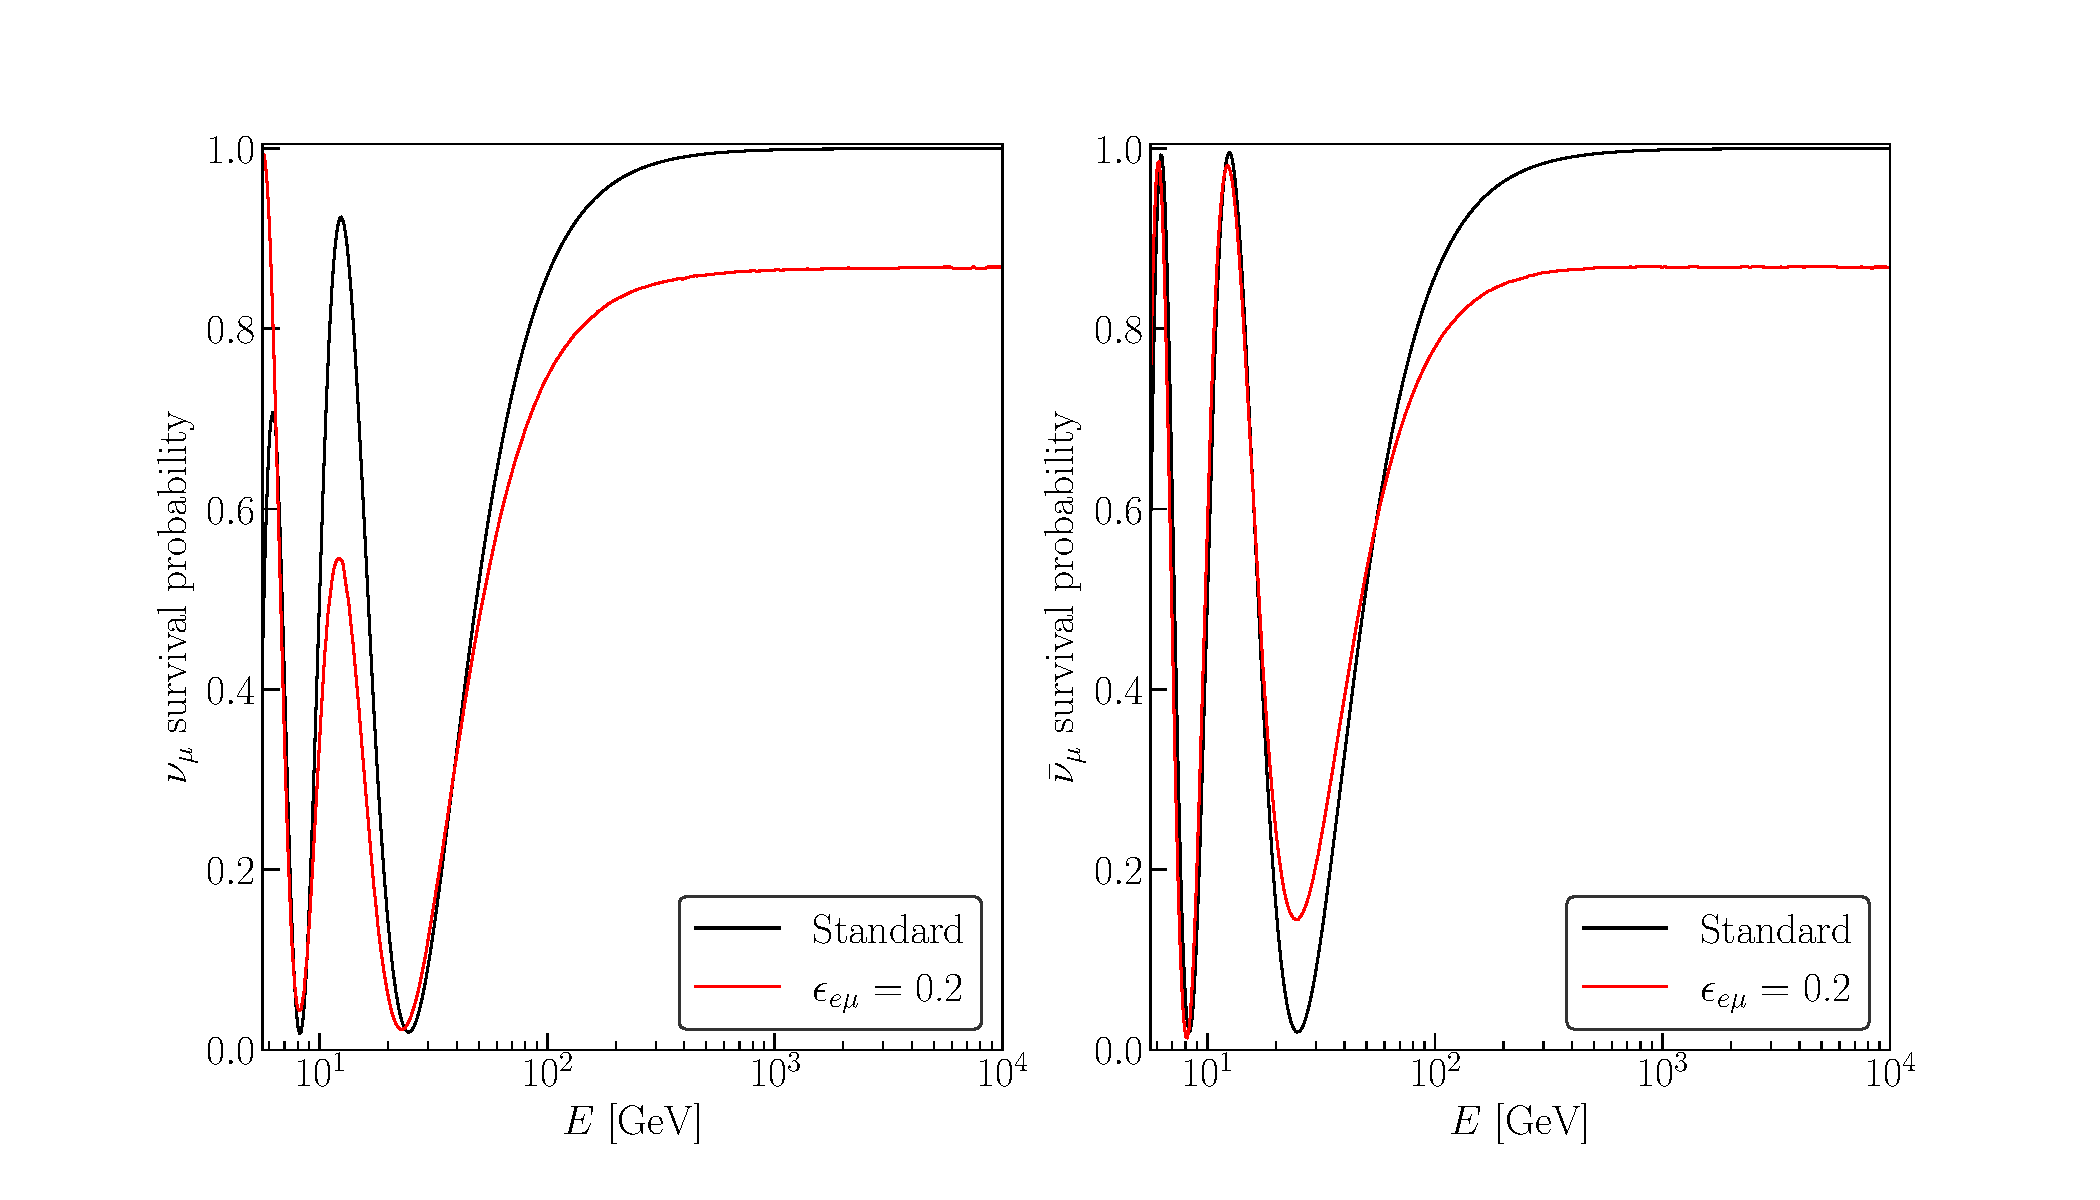
\includegraphics[width=0.99\textwidth]{figures/eem_probs.pdf}
        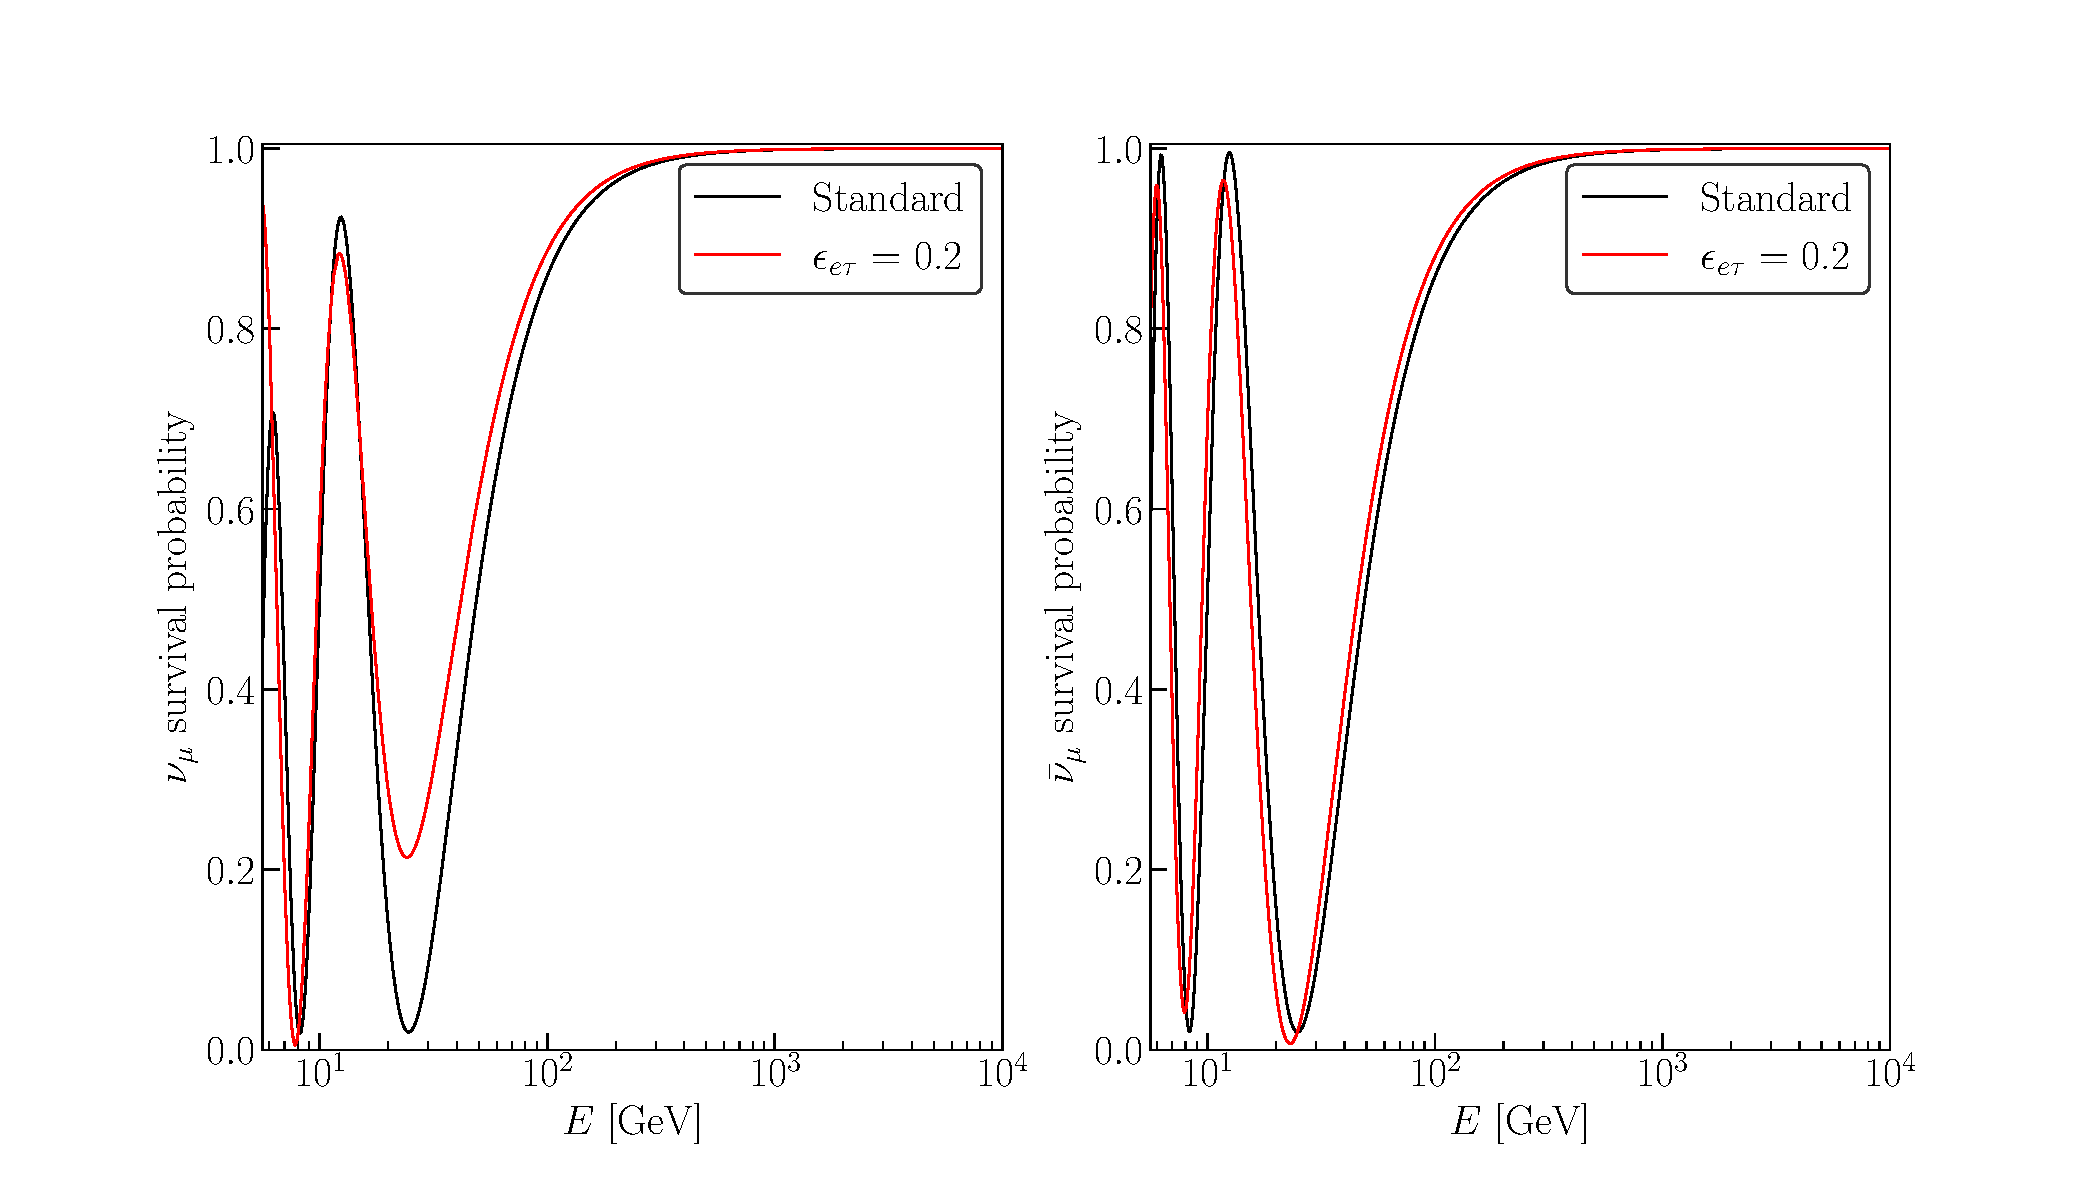
\includegraphics[width=0.99\textwidth]{figures/eet_probs.pdf}
        \caption{Muon neutrino and antineutrino survival probabilities for
        $\ztrue = -1$. \emph{Top panel:} $\eem = 0.2$. All other NSI parameters are fixed to zero. Instead of the oscillations shifting to the left or right, $\eem$ dampens an oscillation peak for low \si{\GeV}. At \si{\TeV}, the probability is shifted down, just as with $\emt$.
        \emph{Bottom panel:} $\eet = 0.2$. All other NSI parameters are fixed to zero. Here, we see a very weak shifting and a $\nm$ weaker dip at low \si{\GeV}, and again, no visible effect at \si{TeV} energies. }
        \label{fig:eem_eet_probs}
    \end{center}
\end{figure}


\subsection{DeepCore and PINGU Signals}
Now we repeat our probability analysis but for the DeepCore/PINGU region of \SIrange{5.6}{56}{\GeV}. As we previously saw,
we have rapid oscillations, which means that `indirect' modifications (i.e. $\eet$ will affect the $\Pmm$ channel)
will be more apparent, since all flavors are involved to a greater degree compared with the more stable region above \SI{500}{\GeV}, where 
many oscillations have averaged out.

Another feature of our DeepCore study includes the fact that we now have access to cascade events, in which $\ne$ and $\nt$ are more abundant.
Thus, we are no longer constrained to the $\mu$ channel alone, but we can now find interesting features in the other channels too. However, we 
remember that the $\nm$ flux is still the most abundant.

Fig.~\ref{fig:Pee_eet_probs} shows the electron neutrino and antineutrino survival probabilities, and here we see
a clear signal when turning on $\eet$. 

\begin{figure}
    \begin{center}
        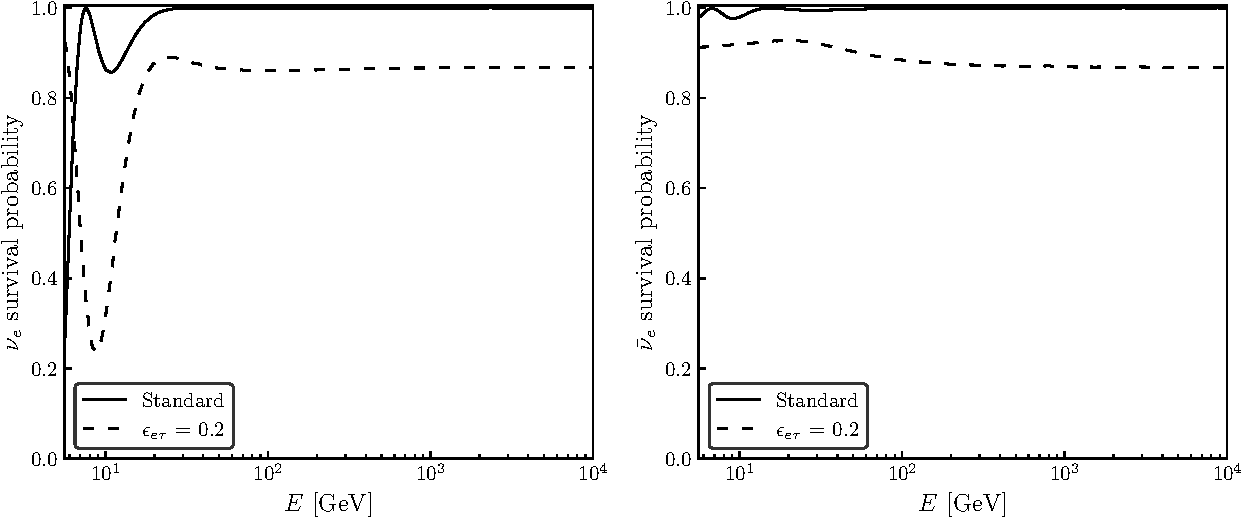
\includegraphics[width=0.9\textwidth]{figures/Pee_eet_probs.pdf}
        \caption{Electron neutrino and antineutrino survival probabilities for
        $\ztrue = -1$ when $\eet = 0.2$. All other NSI parameters are fixed to zero. Here we see a strong difference across the whole energy range, in contrast to the $\nm$ and $\anm$ plots in Fig~\ref{eem_eet_probs}.}
        \label{fig:Pee_eet_probs}
    \end{center}
\end{figure}

Fig.~\ref{fig:emt_ett_probs} shows that $\emt$ affects both $\Pmm$ and $\Pamam$ over the whole energy range. Since 
IceCube also sees this, we hope to be able to boost the constraining of $\emt$ by combining the two experiments.

Regarding $\ett$ in Fig.~\ref{fig:eem_eet_probs}, the signal mainly shows in the $\Pamam$ channel as
a shallower dip in the \SI{20}{\GeV} region. Thus, DeepCore/PINGU alone will be used to constrain this parameter.

$\eem$ in Fig.~\ref{fig:eem_eet_probs} causes a weaker dip for both $\nm$ and $\anm$. 


For $\eet$, we see a similar effect on the dip in $\Pmm$ as we did with $\ett$ for $\Pamam$. Hence, we should be able to 
see the $\eet$ effect in DeepCore/PINGU. Remember that we now have the option to look at the other flavor channels than $\mu$ since we 
have cascade events for DeepCore and PINGU. If we simulate 
$\Pme^{NSI}$ at three different energies, and let both $\eem$ and $\eet$ vary together between the values $\{-0.3,0.3\}$, we produce a two-dimensional grid of probabilities.
Subtract the regular $\Pme^{SI}$ (that is, no NSI), and take the absolute value of the difference. We see the result in Fig.~\ref{fig:eem_eet_prob}. 
The middle and right panels, which show the absolute probability difference at \si{25} and $\SI{50}{\GeV}$, respectively, are very bleak,
indicating that the impact of the NSI parameters $\eem$ and $\eet$ is not as strong at these energy levels. Turning to the left-most panel,
we see a region in which the difference again is close to zero, but now surrounded by fringes of very large differences, up to $50\%$ difference 
in the $\Pme$ probability. This indicating that the NSI parameters are much more influential at these energies, and that we should be able to 
constrain both $\eem$ and $\eet$ from $\SI{5}{\GeV}$ cascade events.

\begin{figure}
    \centering
    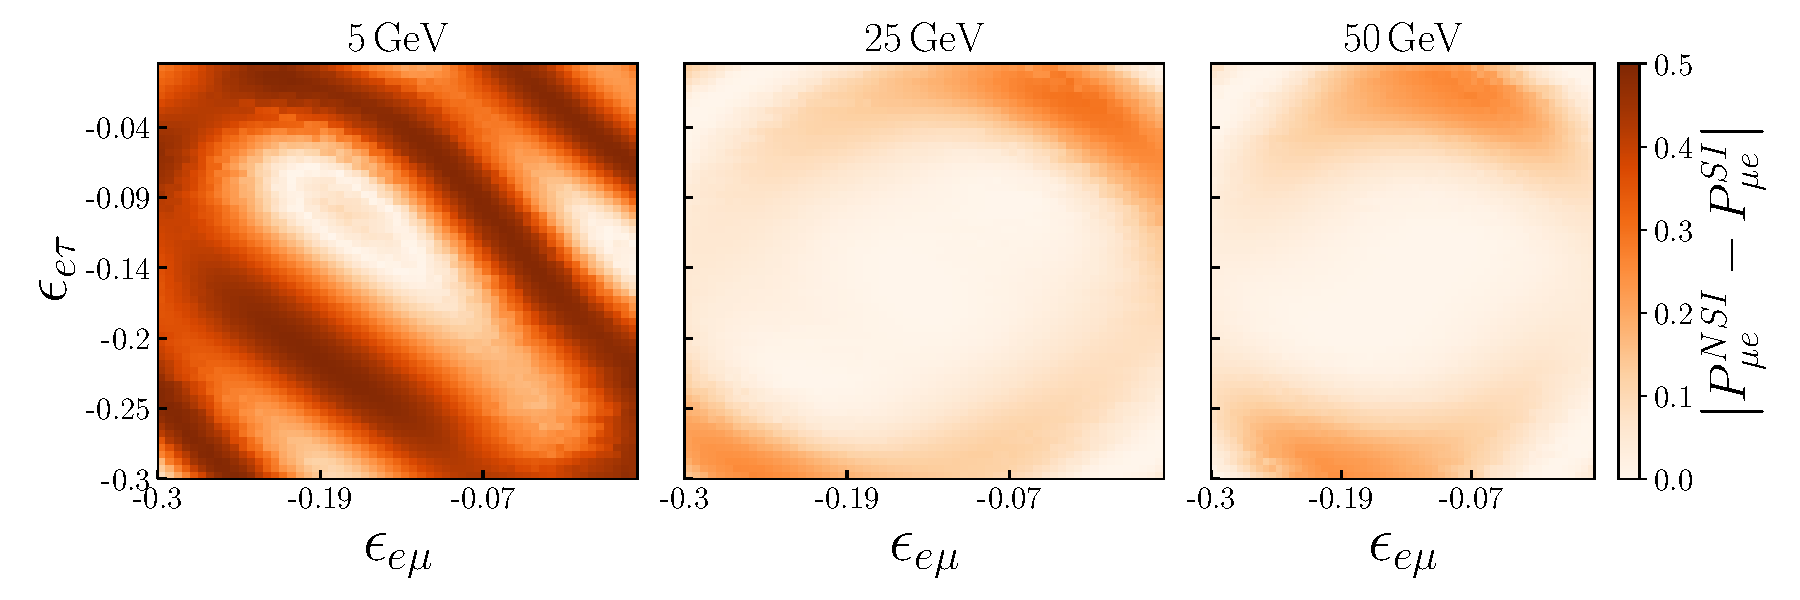
\includegraphics[width=1\textwidth]{figures/eem_eet_prob.pdf}
    \caption{The quantity $\abs{P_{\mu e}^{NSI} - P_{\mu e}^{SI}}$ when we let $\eem$ and $\eet$ independently vary over
    the range \{-0.3,0.3\} at \si{5}, \si{25}, and $\SI{50}{\GeV}$. At $\SI{5}{\GeV}$, we see strong deviations in the probabilities, showing
    a promising indication that constriction of $\eem$ and $\eet$ is possible using cascade events at these energies.}\label{fig:eem_eet_prob}
\end{figure}



\chapter{Results}\label{ch:results}
\section{The Sterile Hypothesis}\label{sec:sterileResults}
With the null ($3\nu$) hypothesis normalized to the IceCube Monte Carlo as in Eq.~\ref{eq:MC_norm}, we are now in good shape to study the sterile neutrino effect on the probabilities, and how that compares to data
\footnote{We do not consider DeepCore nor PINGU in the sterile neutrino analysis because the $\Pamam$ resonance does not appear in the \si{\GeV} region for \si{\eV^2}-scale $\dm[41]$, as shown in Fig.~\ref{fig:sterile_resonance}.
We bring DeepCore and PINGU back in the next section.}.
First, let us see how the collected data from Fig.~\ref{fig:IC_data} deviates from the predicted $3\nu$ oscillations.
\begin{figure}
    \centering
    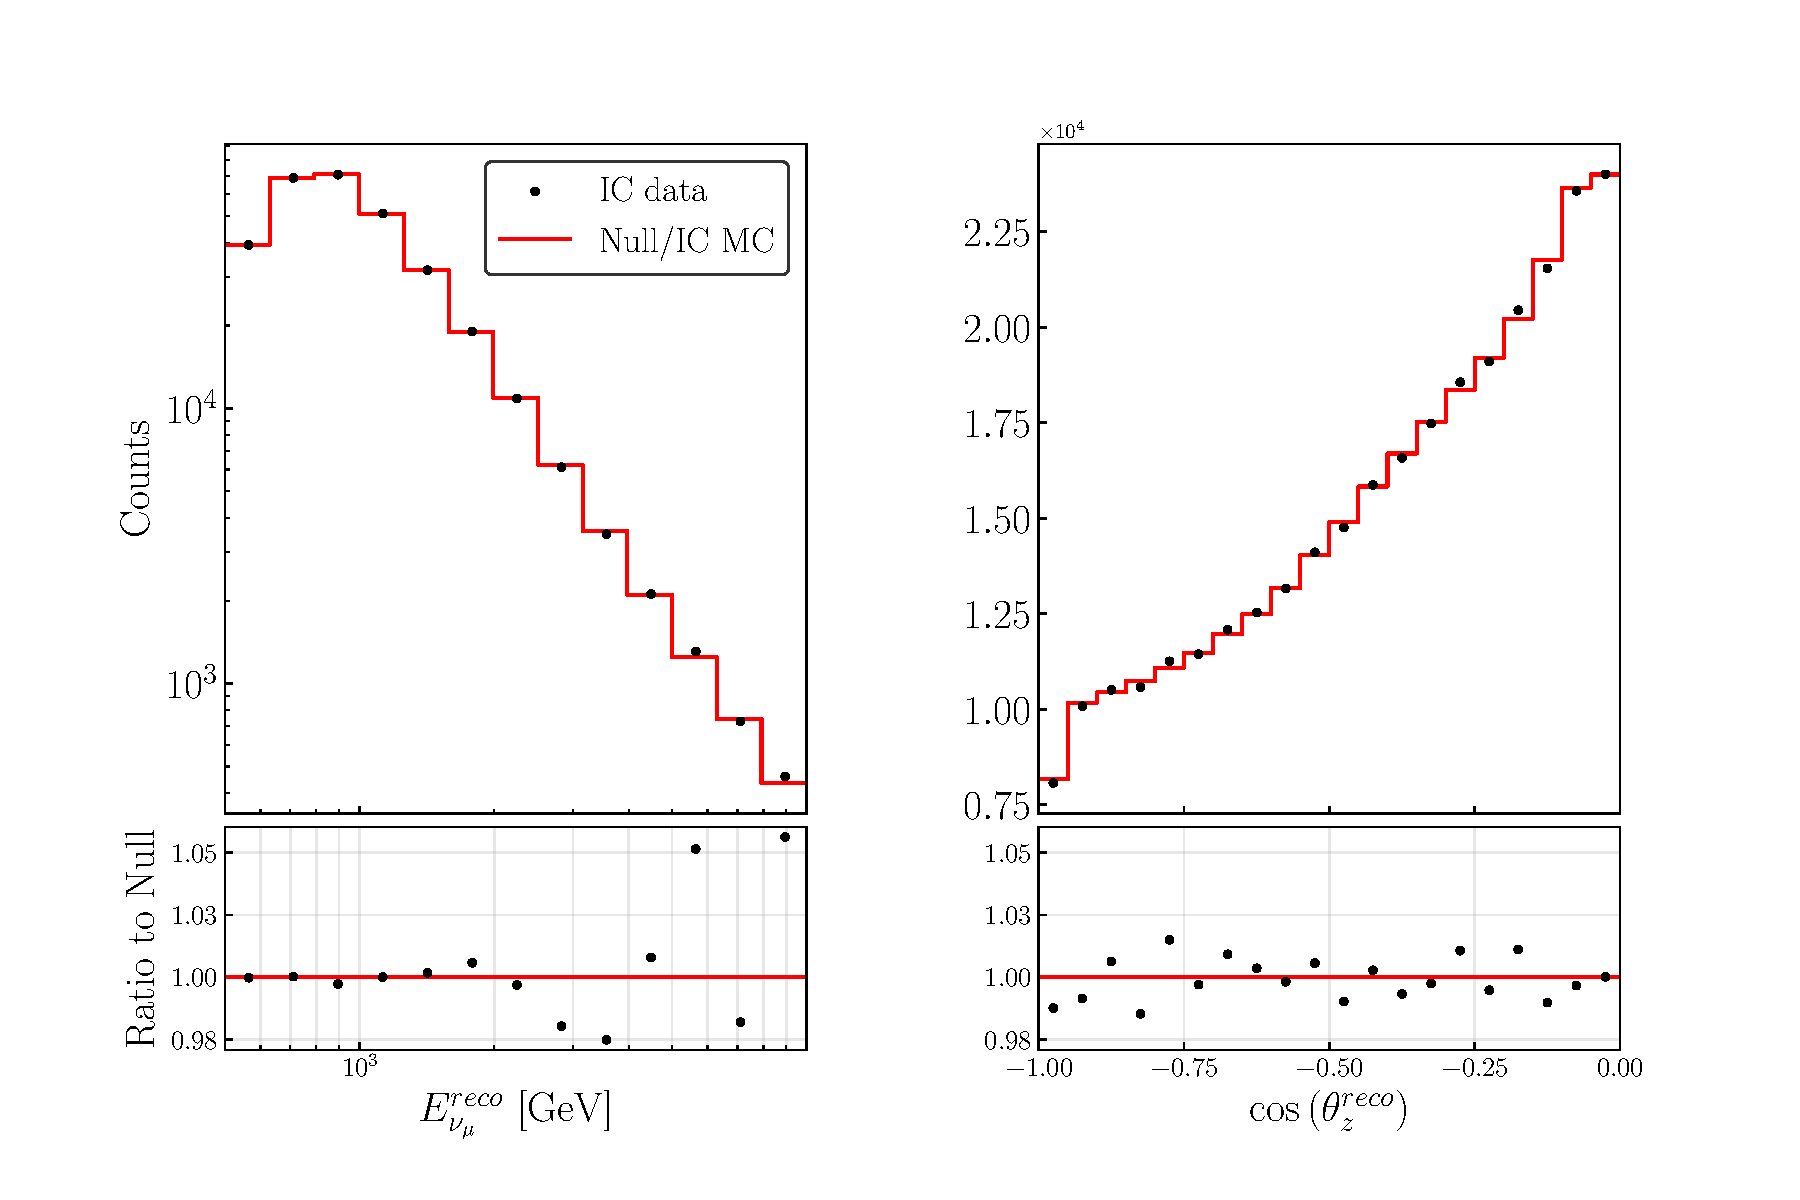
\includegraphics[width=1\textwidth]{figures/IC_rates.pdf}
    \caption{How the IceCube null hypothesis from~\cite{IC2020} compares to their collected data.}\label{fig:IC_rates}
\end{figure}
Fig.~\ref{fig:IC_rates} shows an impressive agreement to the standard $3\nu$ oscillation picture, with the largest deviations of $~6\%$
for neutrinos with high single-digit \si{\TeV} values. In zenith, the data only deviates $\pm 2\%$.


\subsection{\texorpdfstring{$\chi^2$}{Chi-squared} Minimization}
For our analyses, we define our $\chi^2$ as
\begin{align} \label{eq:chisq}
    \chi^{2}(\hat{\theta},\alpha,\beta)=\sum_{ij} \frac{\left(N^\text{th}-N^\text{data}\right)_{ij}^{2}}
    {\left(\sigma^\text{data}_{ij}\right)^{2} + \left(\sigma^\text{syst}_{ij}\right)^{2}}+ 
    \frac{(1-\alpha)^2}{\sigma_\alpha^2} + \frac{\beta^2}{\sigma_\beta^2}\,
\end{align}
where we minimize over the model parameters $\hat{\theta}$, the penalty terms $\alpha$ and $\beta$.
$N_{ij}^\text{th}$ is the expected number of events from theory, and $N_{ij}^\text{data}$ is the observed number of events in that bin. 
We set $\sigma_\alpha = 0.25$ as the atmospheric flux normalization error, and $\sigma_\beta = 0.05$ as the zenith angle slope error~\cite{hondapaper}. 
The observed event number has an associated Poissonian uncertainty $\sigma_{ij}^\text{data} = \sqrt{N_{ij}^\text{data}}$.
For IceCube, the event count takes the form
\begin{align}
    N^\text{th}_{ij} = \alpha\left[1+\beta (0.5 + \zreco_i )\right] N_{ij}(\hat{\theta})\,,
\end{align}
with $N_{ij}(\hat{\theta})$ from Eq.~\ref{eq:MC_norm}. Here, the term $ \beta (0.5 + \zreco_i )$ allows the event distribution to rotate with angle $\beta$ around the median zenith angle of $\zreco = -0.5$.
We also have an uncorrelated systematic error $\sigma_{ijk}^\text{syst}$. We set $\sigma_{ijk}^\text{syst} = f\sqrt{N_{ijk}^\text{data}}$, where $f$ is a factor of our own choosing.

The minimization of Eq.~\ref{eq:chisq} simply returns a value for each set of model parameters. We use this value to quantify to what extent
our theoretical simulations $N^\text{th}_{ij}$ agree with the data $N^\text{data}_{ij}$ within the error bounds provided by $\sigma_a,\sigma_b,$ and $f$.
We then select the set of $\chi^2$ values which are the smallest and our allowed parameters are then their associated $\hat{\theta}$.
We then translate the $\chi^2$ distribution by subtracting the best-fit point, and analyze $\Delta \chi^2 = \chi^2 - \chi^2_{min}$.
From the $\chi^2$-distribution, one can show that the $90\%$ confidence level has a value of $2.71$ for two degrees of freedom. When slicing through the 
two-dimensional grid of $\Delta \chi^2$ at this level, we then obtain a contour plot that tells us what parameter values are within our $90 \%$ confidence level and what regions are not.

\subsection{Sterile Mass and Mixing}
Let us start with looking at the best-fit event distribution resulting from the $\chi^2$ minimization.
Fig.~\ref{fig:final_rate_plot} now contains the best-fit event distribution assuming the 3+1 hypothesis.
The best-fit values are $\dm[41] = \SI{0.01}{\eV\squared}$ and 
$\sin(2\theta_{24})^2 = 0.67$ ($\theta_{24} = \SI{27.5}{\degree}$). %TODO: double check these
The contour plot shown in Fig.~\ref{fig:error_tuning} divides the parameter space into two regions.
To the right of the boundary, the $\Delta \chi^2$ has values above the confidence level, meaning that 
those parameter pairs can be excluded at a certain confidence level.

By tuning the scaling $f$ of the uncorrelated systematic error, we can shift the contour. We extract the contour from the 
IceCube sterile neutrino analysis~\cite{IC2020}, and compare in Fig.~\ref{fig:error_tuning}. We see that the contour in the 
higher $\dm[41]$ region above \SI{1}{\eV\squared} is very sensitive to the tuning, while the lower region between \SIrange[]{1e-1}{1}{\eV\squared}
remains fixed. In both cases, we obtain best-fit values of $\dm[41] = \SI{0.01}{\eV^2}$ and $\theta_{24} = 0.67$ ($\sin^22\theta_{24} = 0.95$) at 
a p-value of $33\%$.
\begin{figure}
    \centering
    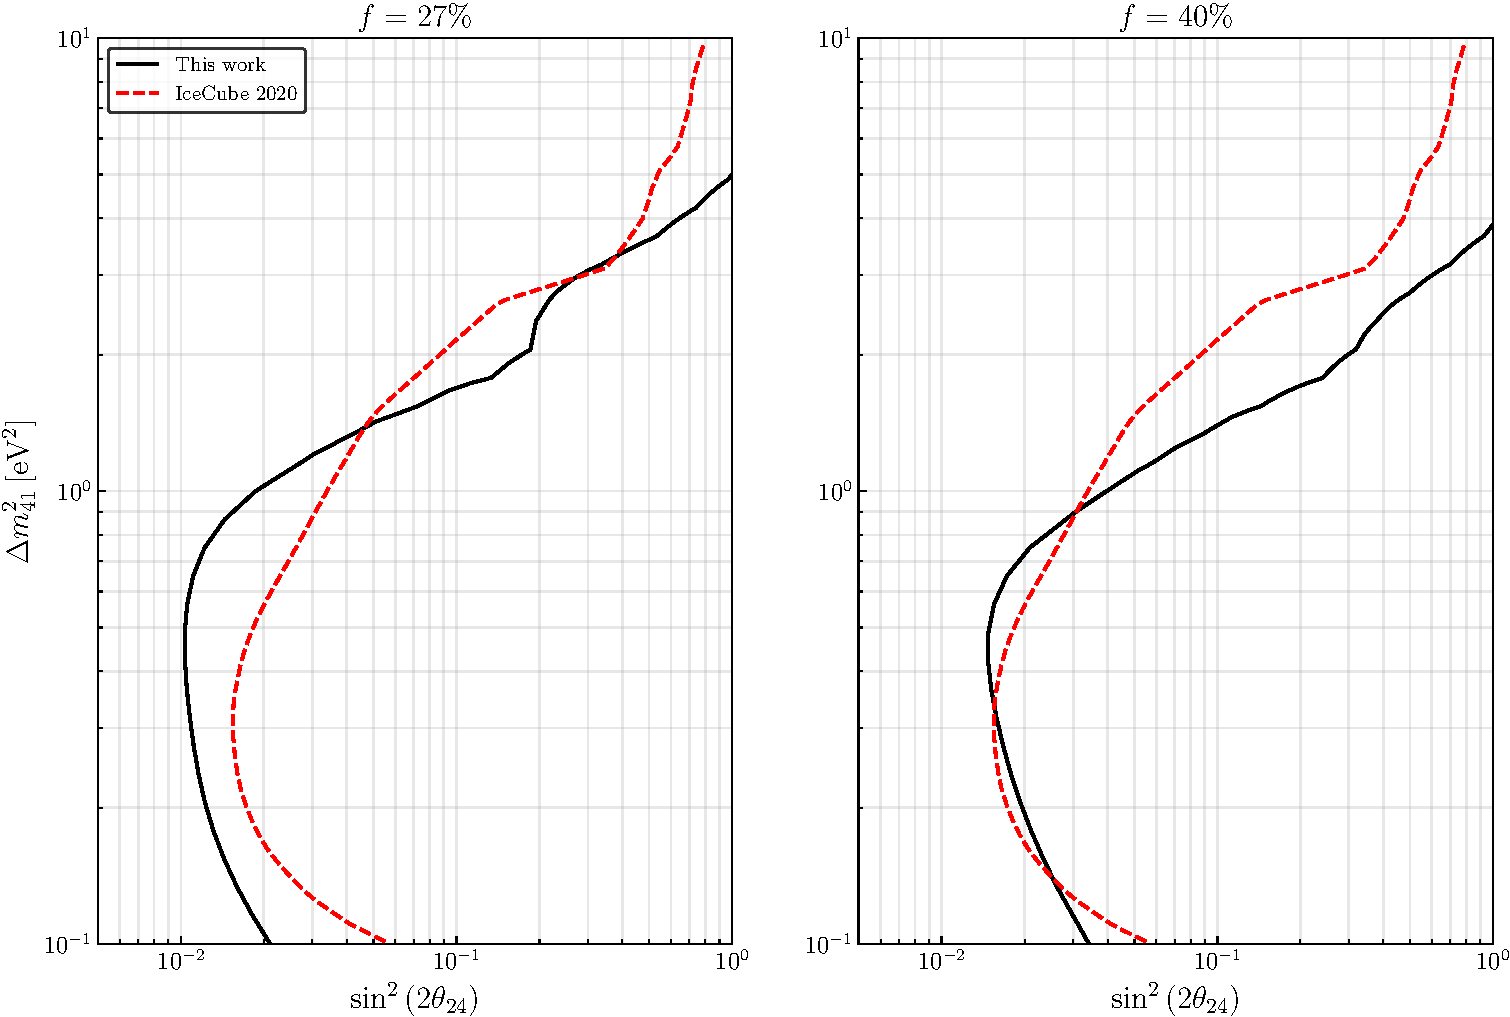
\includegraphics[scale=0.58]{figures/s24_error_tuning.pdf}
    \caption{The 90\% CL contour with two different systematic error scalings, compared 
    with the official IceCube result from~\cite{IC2020}.}\label{fig:error_tuning}
\end{figure}

We now in Fig.~\ref{fig:final_rate_plot} plot the best-fit 3+1 hypothesis with the data from Fig.~\ref{fig:IC_rates}, to finally see how the best 
3+1 hypothesis compares to data.
\begin{figure}
    \centering
    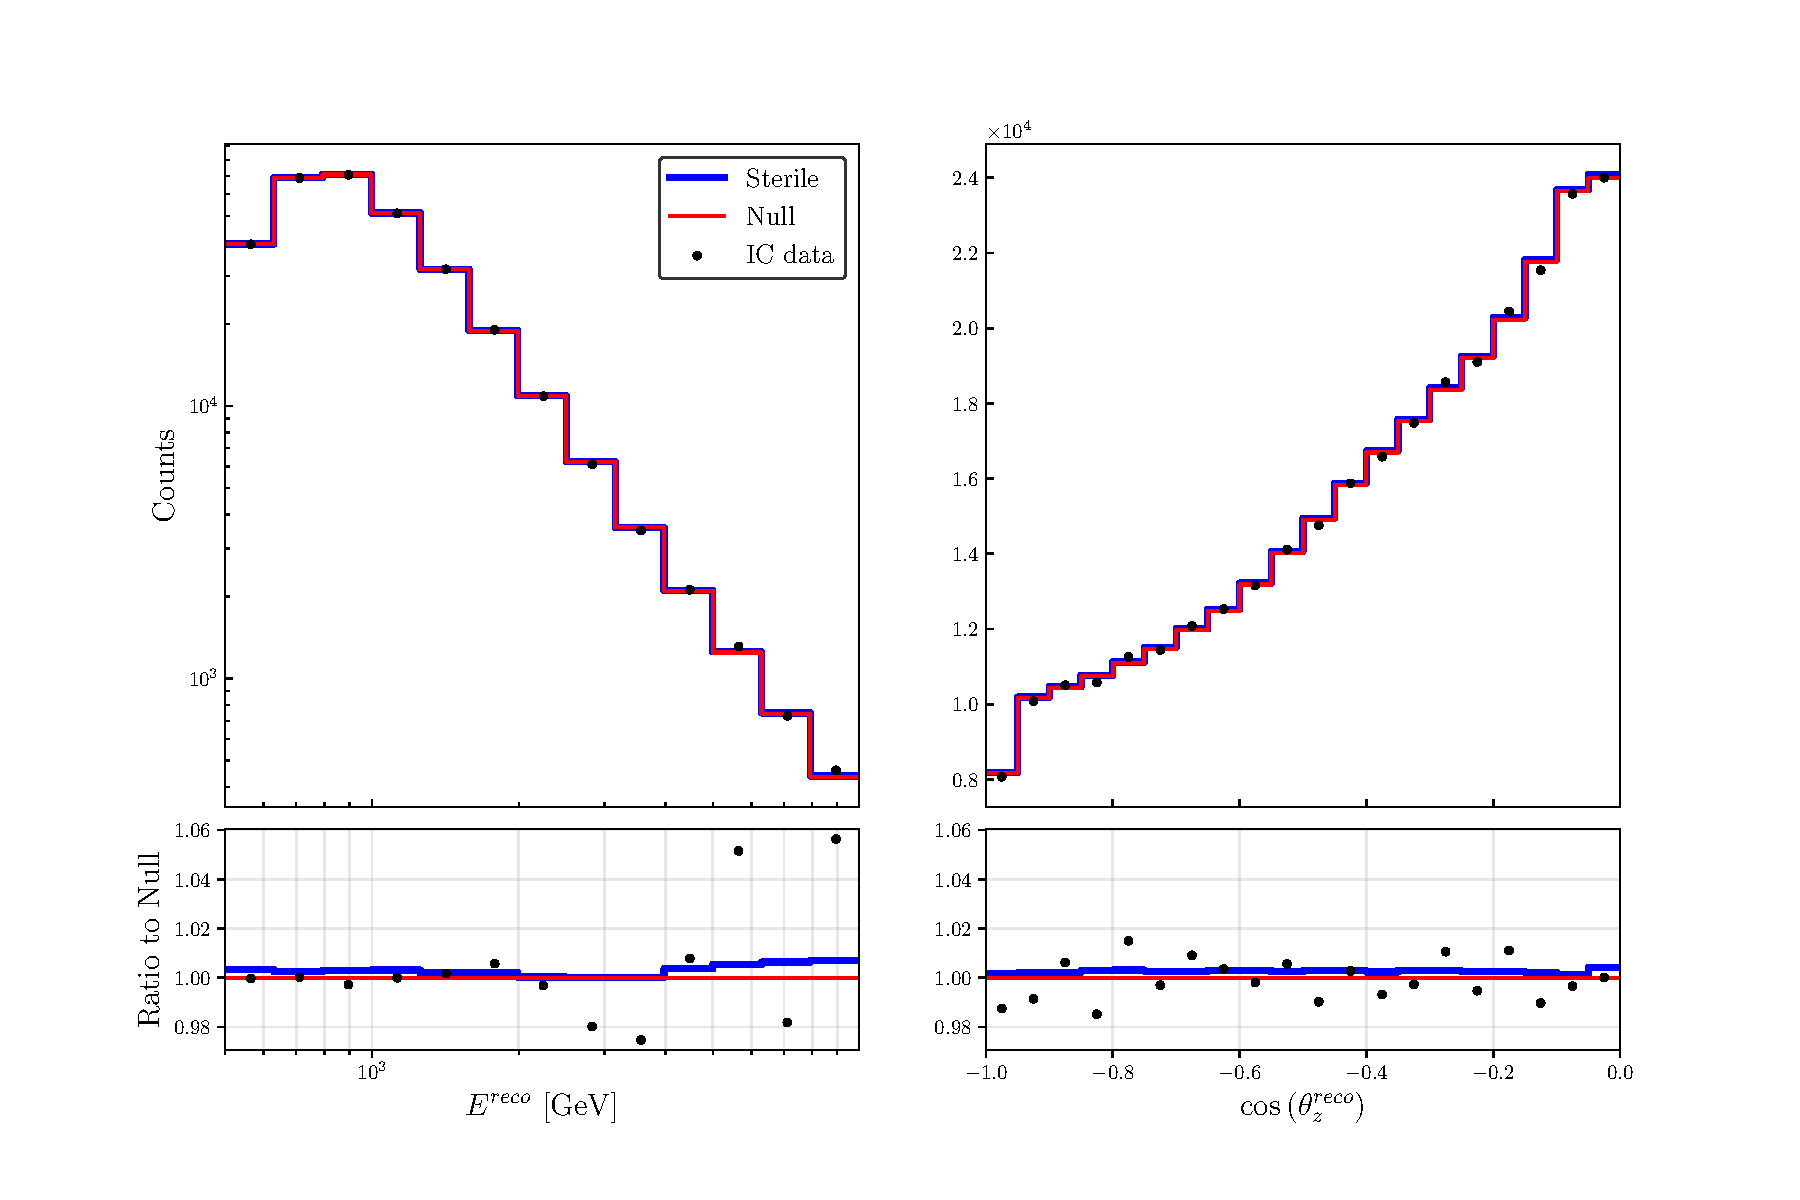
\includegraphics[width=1\textwidth]{figures/final_rate_plot.pdf}
    \caption{The predicted binned event count assuming our best-fit 3+1 hypothesis in blue with $\dm[41] = \SI{0.01}{\eV^2}$ and $\theta_{24} = 0.67$, compared with the 
    null 3+0 hypothesis in red and data points from ~\cite{IC2020} in black.}\label{fig:final_rate_plot}
\end{figure}

In Fig.~\ref{fig:final_rate_plot}, we see that the simulations are consistent with the 3+0 hypothesis with deviations of 6\% at high single-digit 
\si{\TeV} energies.
Wanting to investigate the effect of $\theta_[34]$, we also simulated the 3+1 hypothesis using $\theta_[24] = \theta_[34]$. However, we did not see 
a difference in the exclusion regions compared to the regions when $\theta_[34] = 0$. Thus, we conclude that on our work, IceCube was not able to 
distinguish any effect due to the $\theta_[34]$ parameter.
% \documentclass[draft=True]{thesis}
% \usepackage[margin=0.5in]{geometry}
% \usepackage{graphicx, slashed, siunitx}
% \usepackage[utf8]{inputenc}
% \usepackage{xr-hyper}
% \documentclass[a4paper,10pt,draft]{thesis}
\usepackage{physics,amsmath, amsfonts, siunitx, amssymb, graphicx, slashed,subcaption}
\usepackage[utf8]{inputenc}
\usepackage[margin=1in]{geometry}
\usepackage[hidelinks]{hyperref}
\usepackage{xr-hyper}
\newcommand{\n}[1]{\nu_{#1}}
\newcommand{\na}{\nu_\alpha}
\newcommand{\nb}{\nu_\beta}
\newcommand{\ana}{\bar{\nu}_\alpha}
\newcommand{\an}[1]{\bar{\nu}_{\text{#1}}}
\newcommand{\anb}{\bar{\nu}_\beta}
\renewcommand{\a}{\alpha}
\renewcommand{\b}{\beta}
\newcommand{\ab}{\alpha\beta}


\renewcommand{\ne}{\nu_e}
\newcommand{\nm}{\nu_\mu}
\newcommand{\nt}{\nu_\tau}
\newcommand{\ns}{\nu_s}

\newcommand{\ane}{\bar{\nu}_e}
\newcommand{\anm}{\bar{\nu}_\mu}
\newcommand{\ant}{\bar{\nu}_\tau}
\newcommand{\ans}{\bar{\nu}_s}

\newcommand{\nee}{\nu_e \to \nu_e}
\newcommand{\nem}{\nu_e \to \nu_\mu}
\newcommand{\net}{\nu_e \to \nu_\tau}
\newcommand{\nes}{\nu_e \to \nu_s}

\newcommand{\nme}{\nu_\mu \to \nu_e}
\newcommand{\nmm}{\nu_\mu \to \nu_\mu}
\newcommand{\nmt}{\nu_\mu \to \nu_\tau}
\newcommand{\nms}{\nu_\mu \to \nu_s}



\newcommand{\Pee}{P_{e  e}}
\newcommand{\Pem}{P_{e  \mu}}
\newcommand{\Pet}{P_{e  \tau}}
\newcommand{\Pes}{P_{e  s}}

\newcommand{\Pme}{P_{\mu  e}}
\newcommand{\Pmm}{P_{\mu\mu}}
\newcommand{\Pmt}{P_{\mu  \tau}}
\newcommand{\Pms}{P_{\mu  s}}


\newcommand{\Pte}{P_{P_{\tau e}}}
\newcommand{\Ptm}{P_{\tau  \mu}}
\newcommand{\Ptt}{P_{\tau  \tau}}
\newcommand{\Pts}{P_{\mu  s}}

\newcommand{\Paeae}{P_{\bar{e}  \bar{e}}}
\newcommand{\Paeam}{P_{\bar{e}  \bar{\mu}}}
\newcommand{\Paeat}{P_{\bar{e}  \bar{\tau}}}
\newcommand{\Paeas}{P_{\bar{e}  \bar{s}}}

\newcommand{\Pamae}{P_{\bar{\mu}  \bar{e}}}
\newcommand{\Pamam}{P_{\bar{\mu}  \bar{\mu}}}
\newcommand{\Pamat}{P_{\bar{\mu}  \bar{\tau}}}
\newcommand{\Pamas}{P_{\bar{\mu}  \bar{s}}}


\newcommand{\Patae}{P_{\bar{\tau}  \bar{e}}}
\newcommand{\Patam}{P_{\bar{\tau}  \bar{\mu}}}
\newcommand{\Patat}{P_{\bar{\tau}  \bar{\tau}}}
\newcommand{\Patas}{P_{\bar{\mu}  \bar{s}}}

\renewcommand{\th}[1][]{%
  \theta\ifx\\#1\\\else_\text{#1}\fi
}
\newcommand{\thm}[1][]{%
  \theta^\text{M}\ifx\\#1\\\else_\text{#1}\fi
}
\renewcommand{\t}[1]{\text{{#1}}}
\newcommand{\avg}[1]{\left\langle {#1} \right \rangle}
\newcommand*{\dm}[1][]{%
  \Delta m^2\ifx\\#1\\\else_\text{#1}\fi
}
\newcommand{\zreco}{\cos{(\theta_z^{reco})}}
\newcommand{\ztrue}{\cos{(\theta_z^{true})}}
\newcommand{\z}{\cos{(\theta_z)}}
\newcommand{\Ereco}{E^{reco}}
\newcommand{\Etrue}{E^{true}}
\newcommand{\Aeff}{A^\text{eff}}
\newcommand{\emm}{\epsilon_{\mu\mu}}
\newcommand{\emt}{\epsilon_{\mu\tau}}
\newcommand{\eet}{\epsilon_{e\tau}}
\newcommand{\eem}{\epsilon_{e\mu}}
\newcommand{\ett}{\epsilon_{\tau\tau}}
\newcommand{\ep}{\epsilon^\prime}

% \begin{document}
\section{Non-Standard Interactions}\label{sec:nsiResults}
\subsection{Constraining the NSI parameters}\label{sec:constraining}
In this section, we will constrain the four NSI parameters $\ett$, $\emt$, $\eem$, and $\eet$ by considering the detectors separately as well as jointly.
For our analyses, we define our $\chi^2$ as
\begin{align} \label{eq:chisq}
    \chi^{2}(\hat{\theta},\alpha,\beta, \kappa)=\sum_{ijk} \frac{\left(N^\text{th}-N^\text{data}\right)_{ijk}^{2}}
    {\left(\sigma^\text{data}_{ijk}\right)^{2} + \left(\sigma^\text{syst}_{ijk}\right)^{2}}+ 
    \frac{(1-\alpha)^2}{\sigma_\alpha^2} + \frac{\beta^2}{\sigma_\beta^2}\,
\end{align}
where we minimize over the model parameters $\hat{\theta} \in \{\dm, \theta_{23}, \epsilon\}$, the penalty terms $\alpha$ and $\beta$, and the free parameter $\kappa$.
$N_{ijk}^\text{th}$ is the expected number of events from theory, and $N_{ijk}^\text{data}$ is the observed number of events in that bin. 

In our simulations of $N_{ijk}^\text{th}$, we set all standard oscillation parameters to their current best-fit values of Eq.~\ref{eq:PINGUparams}, 
except for $\dm$ and $\theta_{23}$
which we vary over their $3\sigma$ limits \SIrange{2.435e-3}{2.598e-3}{\eV \squared} and \SIrange{40.1}{51.7}{\degree}, respectively.

We set $\sigma_\alpha = 0.25$ as the atmospheric flux normalization error, and $\sigma_\beta = 0.04$ as the zenith angle slope error~\cite{hondapaper}. 
The observed event number has an associated Poissonian uncertainty $\sigma_{ijk}^\text{data} = \sqrt{N_{ijk}^\text{data}}$.
For IceCube, the event count takes the form
\begin{align}
    N^\text{th}_{ij} = \alpha\left[1+\beta (0.5 + \zreco_i )\right] N_{ij}(\hat{\theta})\,,
\end{align}
with $N_{ij}(\hat{\theta})$ from Eq.~\ref{eq:ICevents}. Here, we allow the event distribution to rotate around the median cosine-zenith of $\zreco = -0.5$.

For DeepCore and PINGU, and the event count takes the form
\begin{align}
    N^\text{th}_{ijk} = \alpha\left[1+\beta \zreco_i \right] N_{ijk}(\hat{\theta}) + \kappa N_{ijk}^{\mu_{atm}}\,,
\end{align}
with $N_{ijk}(\hat{\theta})$ from Eq.~\ref{eq:MCevents}. $N_{ijk}^{\mu_{atm}}$ is the muon background, which is left to float freely in the DeepCore analysis.
The background at PINGU can be considered negligible to first order~\cite{PINGUdata}, and we thus put $\kappa=0$ when calculating the PINGU $\chi^2$.
For DeepCore and PINGU, the median cosine-zenith is $\zreco = 0$, and we allow the event count to rotate around this point.

We treat the uncorrelated systematic uncertanties differently for each detector. For IceCube, we set $\sigma_{ijk}^\text{syst} = f\sqrt{N_{ijk}^\text{data}}$.
We consider best, normal, and worst-case scenarios in IceCube using
$f=5\%$, $10\%$, and $15\%$ respectively. For PINGU, we use the same form but instead use $f=0\%$, $3\%$, and $5\%$. %TODO: maybe source/justification for these values?
For DeepCore, we use the provided systematic error distribution which accounts for uncertainties in the finite MC statistics and the data-driven 
muon background estimate~\cite{DC2019data}. This is summarized in Table~\ref{table:syst_errors}.  %TODO segue
{\renewcommand{\arraystretch}{1.2}
\begin{table}
   \begin{tabular}{lccc}
      \hline \hline
      Experiment & Best case & Baseline & Worst case \\
      \hline
      IceCube & $5\%$ & $10\%$ & $15\%$ \\
      PINGU & $0\%$ & $3\%$ & $5\%$ \\
      \hline \hline
   \end{tabular}
   \caption{Our definition of the best, baseline, and worst case scenarios considered in each experiment, modelled by $\sigma_{ijk}^\text{syst} = f\sqrt{N_{ijk}^\text{data}}$ with $f$ from the table.
   We do not consider different DeepCore scenarios because her systematic error distribution is already provided in the data release~\cite{DC2019data}.}\label{table:syst_errors}
\end{table}

For the joint analysis, we follow the parameter goodness-of-fit prescription~\cite{maltoni2003} and construct the joint $\chi^2$ as 
\begin{align}\label{eq:joint_chisq}
    \chi^2_\text{joint} = \sum_\text{exp}\chi^2_\text{exp} - \chi^2_\text{exp,min}\,
\end{align}
with test statistic $\chi^2_\text{joint,min}$. The $\Delta \chi^2_\text{joint}$ is then $\Delta \chi^2_\text{joint} = \chi^2_\text{joint} - \chi^2_\text{joint,min}$.

After the oscillation parameters have been marginalized out, we plot $\Delta \chi^2$ for each of the four NSI parameters in Fig.~\ref{fig:3D_NO}. 
The results are shown in Fig.~\ref{fig:IC_3D} and summarized in Tables~\ref{table:IC_DC_results} and~\ref{table:PINGU_joint_results}.

Comparing the PINGU and the DeepCore results in Fig.~\ref{fig:3D_NO}, we note that the best-fit for each NSI parameter for the PINGU experiment is expected to be zero. This is because the `data' we generated during 
the PINGU simulations assume no NSI since they have yet to be observed in nature. This introduces a non-NSI bias in all joint analyses which include PINGU,
since PINGU has stronger statistics than DeepCore and will thus pull the joint $\chi^2$ towards $\epsilon =0$.

\begin{figure}
   \begin{center}
      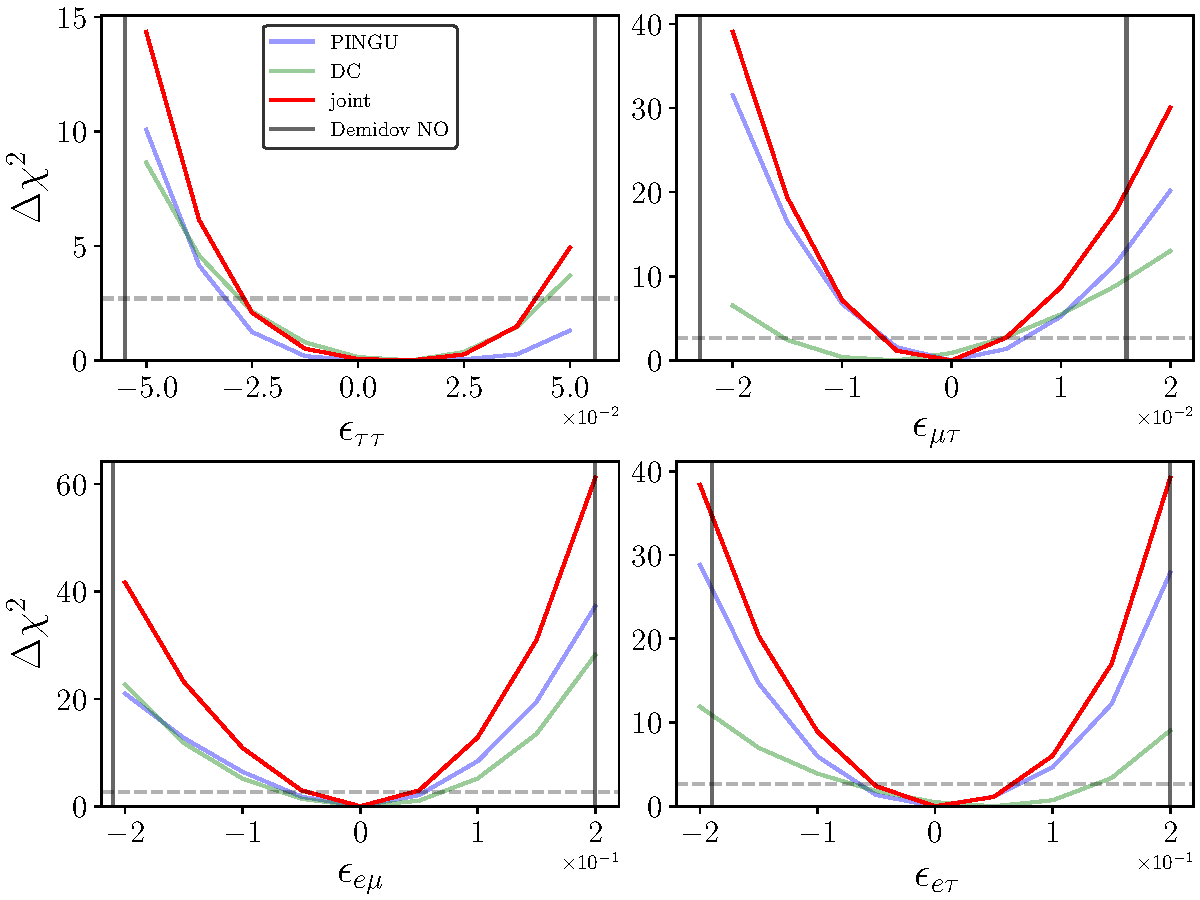
\includegraphics[width=0.6\textwidth]{figures/joint_3D_NO.pdf}
      \caption{PINGU and DeepCore best-case scenario, with their joint $\Delta \chi^2$ in black. $\dm$ and $\theta_{23}$ and have been marginalized out, and all other NSI 
      parameters not shown in each panel are fixed to zero. 
      IceCube tracks only reveal $\emt$, and are displayed separately in Fig.~\ref{fig:IC_3D}.}\label{fig:3D_NO}
   \end{center}
\end{figure} 
\begin{figure}
   \begin{center} 
      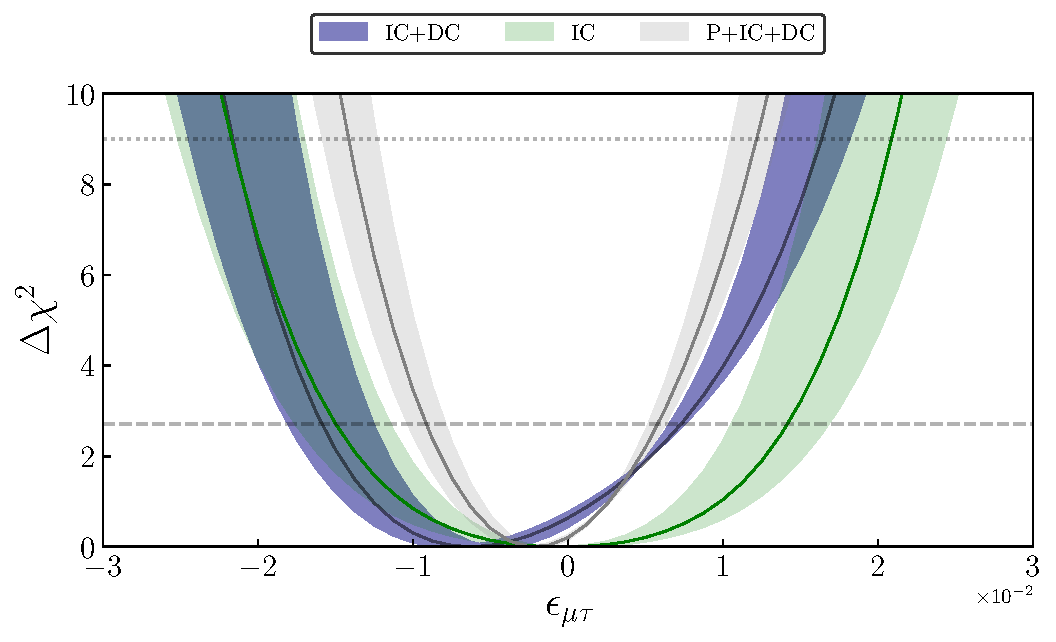
\includegraphics[width=0.6\textwidth]{figures/PID_3D_emt.pdf}
      \caption{$\emt$ $\Delta \chi^2$ regions for scenarios as defined in Table~\ref{table:syst_errors}.
    $\dm$ and $\theta_{23}$ and have been marginalized out, and all other NSI 
    parameters other than $\emt$ are fixed to zero.}\label{fig:IC_3D}
   \end{center}
\end{figure}



{\renewcommand{\arraystretch}{1.3}
 \begin{table}
   \begin{center}
   \begin{tabular}{lcccccc}
      \hline \hline
      Parameter & Best 90\% CL & Best $3\sigma$& Baseline 90\% CL & Baseline $3\sigma$ & Worst 90\% CL & Worst $3\sigma$\\
      \hline & \multicolumn{6}{c}{IceCube}  \\
      $\emt$ &  [-0.008, 0.009] &  [-0.014, 0.017] &   [-0.009, 0.01] &  [-0.015, 0.018] &   [-0.01, 0.011] &   [-0.017, 0.02] \\\\
      & \multicolumn{6}{c}{DeepCore}\\ [0.3em]
      $\ett$ &  [-0.044, 0.051] &  [-0.062, 0.069] &  [-0.046, 0.054] &         [-0.065] &  [-0.049, 0.057] &          [-0.07] \\
      $\emt$ &  [-0.008, 0.009] &  [-0.014, 0.017] &   [-0.009, 0.01] &  [-0.015, 0.018] &   [-0.01, 0.011] &   [-0.017, 0.02] \\
      $\eem$ &  [-0.079, 0.081] &   [-0.16, 0.14] &  [-0.11, 0.094] &  [-0.20, 0.16] &   [-0.14, 0.11] &   [-0.23, 0.18] \\
      $\eet$ &  [-0.079, 0.098] &  [-0.15, 0.16] &   [-0.10, 0.11] &  [-0.19, 0.18] &  [-0.13, 0.13] &  [-0.23, 0.12] \\\\
      &\multicolumn{6}{c}{IceCube + DeepCore}\\
      $\emt$ &  [-0.029, 0.007] &          [0.026] &  [-0.029, 0.007] &          [0.026] &  [-0.029, 0.007] &          [0.026] \\
      \hline
      \hline
   \end{tabular}
   \end{center}
   \caption{IceCube and DeepCore results from the $\Delta \chi^2$ in Fig.~\ref{fig:IC_3D}. Best, baseline, and worst refer to 
   the systematic uncertainty scenarios considered as in Table~\ref{table:syst_errors}.}\label{table:IC_DC_results}
\end{table}
\begin{table}
   \begin{tabular}{lcccccc}
      \hline \hline
      Parameter & Best 90\% CL & Best $3\sigma$& Baseline 90\% CL & Baseline $3\sigma$ & Worst 90\% CL & Worst $3\sigma$\\
      \hline & \multicolumn{6}{c}{PINGU} \\
      $\ett$ &  [-0.054, 0.067] &               [] &  [-0.054, 0.067] &               [] &  [-0.054, 0.067] &               [] \\
      $\emt$ &  [-0.029, 0.007] &          [0.026] &  [-0.029, 0.007] &          [0.026] &  [-0.029, 0.007] &          [0.026] \\
      $\eem$ &  [-0.12, 0.15] &  [-0.23, 0.24] &  [-0.12, 0.15] &  [-0.23, 0.24] &  [-0.12, 0.15] &  [-0.23, 0.24] \\
      $\eet$ &   [-0.084, 0.15] &  [-0.19, 0.21] &   [-0.084, 0.15] &  [-0.19, 0.21] &   [-0.084, 0.15] &  [-0.19, 0.21] \\\\
      & \multicolumn{6}{c}{DeepCore + PINGU} \\
      $\ett$ &  [-0.036, 0.046] &  [-0.056, 0.064] &  [-0.038, 0.048] &  [-0.058, 0.067] &   [-0.039, 0.05] &          [-0.06] \\
      $\emt$ &  [-0.009, 0.006] &  [-0.015, 0.013] &   [-0.01, 0.006] &  [-0.016, 0.014] &  [-0.011, 0.007] &  [-0.017, 0.015] \\
      $\eem$ &   [-0.06, 0.077] &  [-0.126, 0.127] &  [-0.071, 0.086] &  [-0.149, 0.141] &  [-0.082, 0.097] &  [-0.17, 0.16] \\
      $\eet$ &  [-0.052, 0.095] &  [-0.112, 0.144] &  [-0.061, 0.103] &  [-0.131, 0.155] &  [-0.067, 0.11] &  [-0.15, 0.17] \\\\
      & \multicolumn{6}{c}{IceCube + DeepCore + PINGU}  \\
      $\emt$ &  [-0.009, 0.006] &  [-0.015, 0.013] &   [-0.01, 0.006] &  [-0.016, 0.014] &  [-0.011, 0.007] &  [-0.017, 0.015] \\
      \hline
      \hline
   \end{tabular}
   \caption{PINGU and joint results from the $\Delta \chi^2$ in Fig.~\ref{fig:3D_NO}. Best, baseline, and worst refer to 
   the systematic uncertainty scenarios considered as in Table~\ref{table:syst_errors}.}\label{table:PINGU_joint_results}
\end{table}

\begin{table}
   \begin{center}
   \begin{tabular}{lccc}
           \hline \hline & \multicolumn{3}{c} {\text {Best fit}} \\
           \cline { 2 - 4 } Parameter & $\dm$ & $\theta_{23}$  & $\epsilon$  \\
           \hline \multicolumn{3}{c} {\hspace{2.5cm} DeepCore }  \\[0.1em]
           $\ett$ &  2.435 & 47.84 & 0.0125 \\
           $\emt$ &  2.435 & 43.97 & -0.005 \\
           $\eem$ &  2.435 & 43.97 & 0 \\
           $\eet$ &  2.435 & 43.97  & 0.05 \\\\
           \multicolumn{3}{c} {\hspace{2.5cm} IceCube } \\
           $\emt$ &  2.435 & 51.70 & 0 \\
           \multicolumn{3}{c} {\hspace{2.5cm} IceCube + DeepCore } \\
           $\emt$ &  2.517 & 43.97 & -0.01 \\
           \hline
           \hline
   \end{tabular}
   \end{center}
   \caption{Best fit points for $\dm$ and $\theta_{23}$ are given in units of $\si{10^{-3}\eV\squared}$ and
   degrees, respectively.}\label{table:bestfit}
\end{table}
\newpage


 \begin{figure}[t]
   \begin{center}
      \begin{subfigure}{0.38\textwidth}
         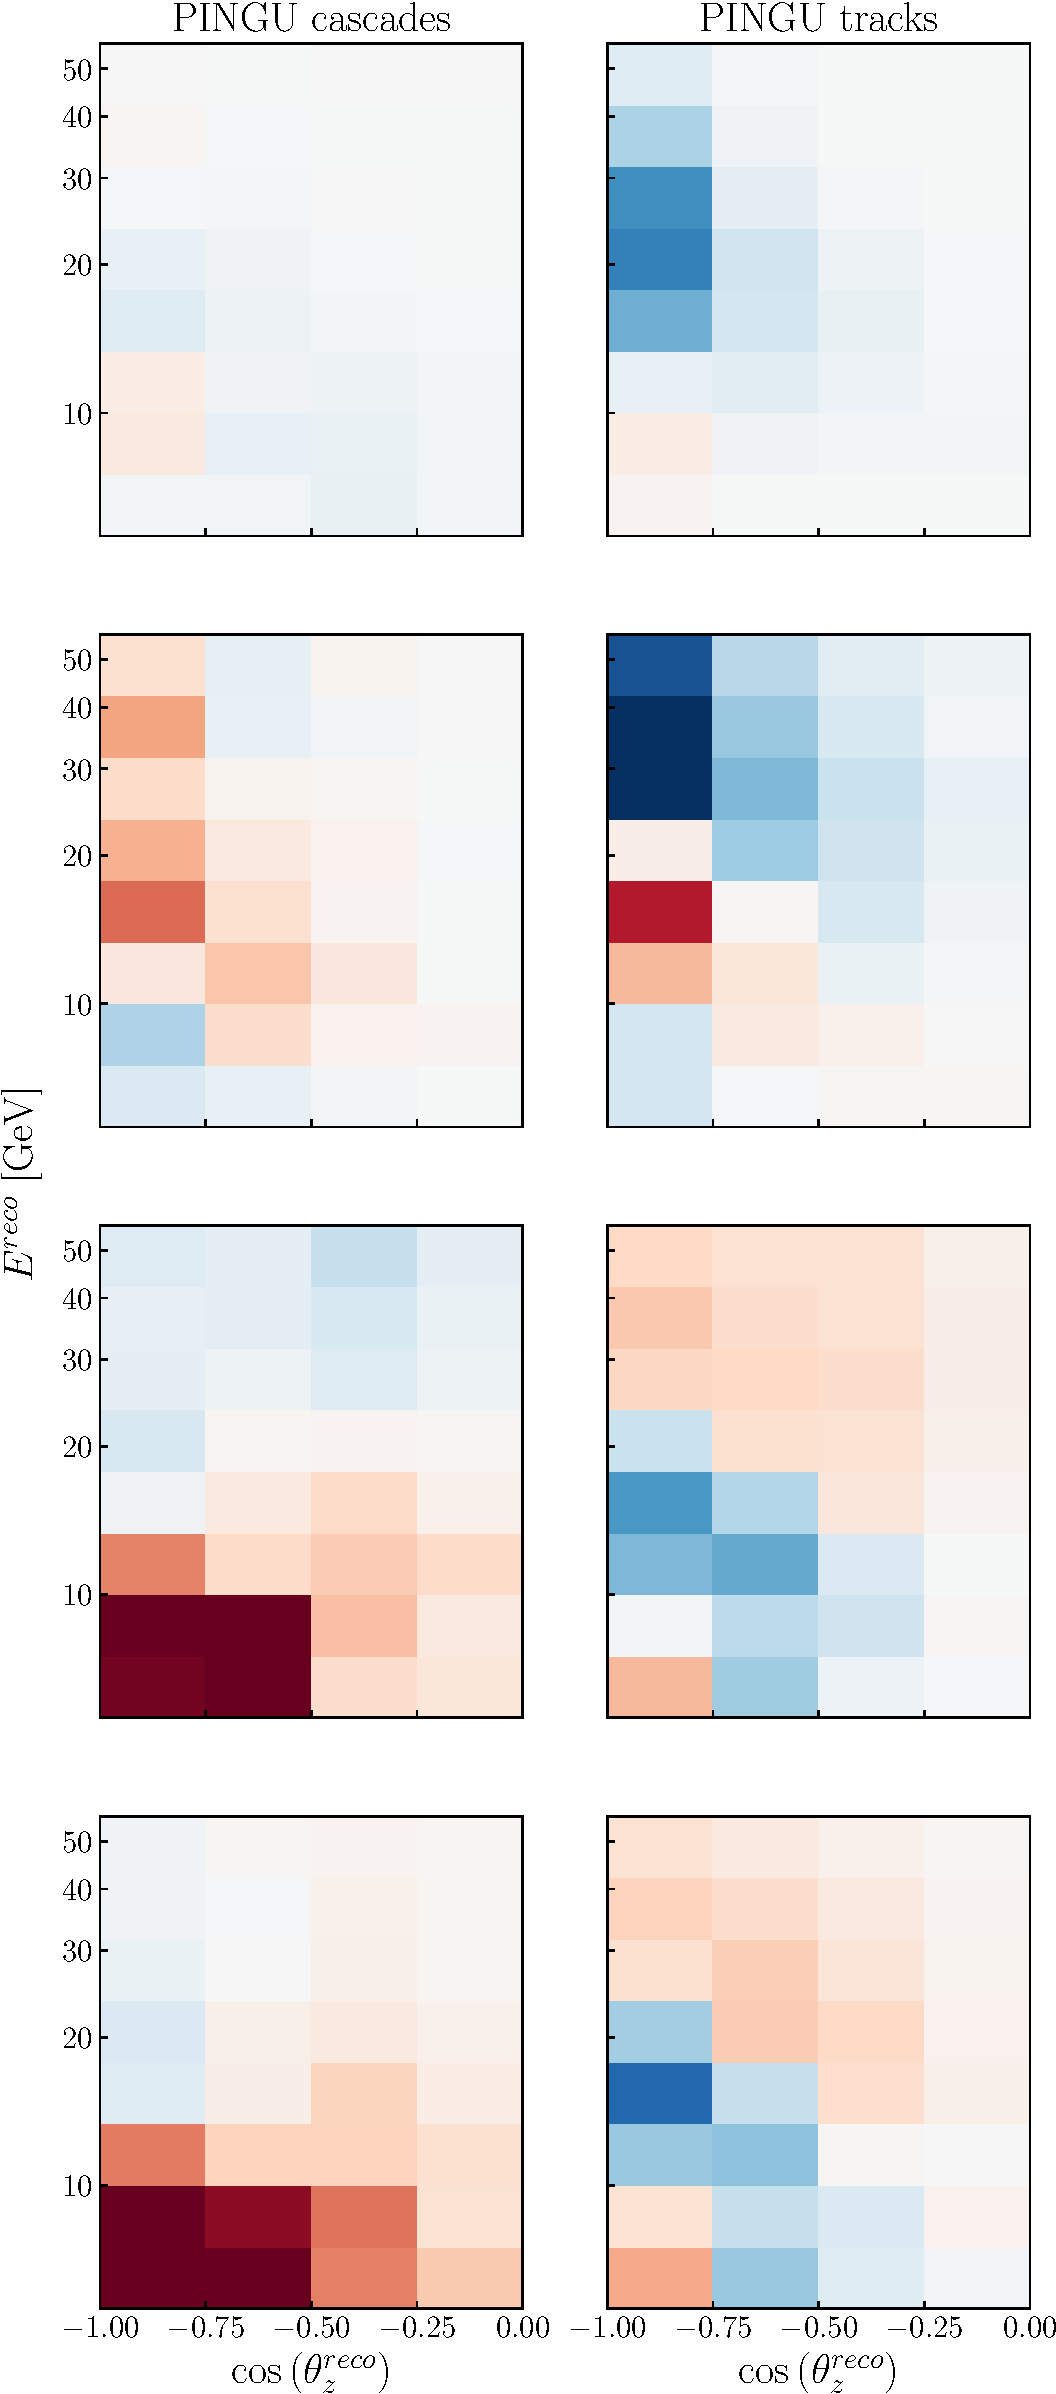
\includegraphics[width=1\linewidth]{figures/PINGU_event_pulls.pdf}
         \caption{PINGU}\label{fig:PINGU_event_pulls}
      \end{subfigure}
      \begin{subfigure}{0.4\textwidth}
         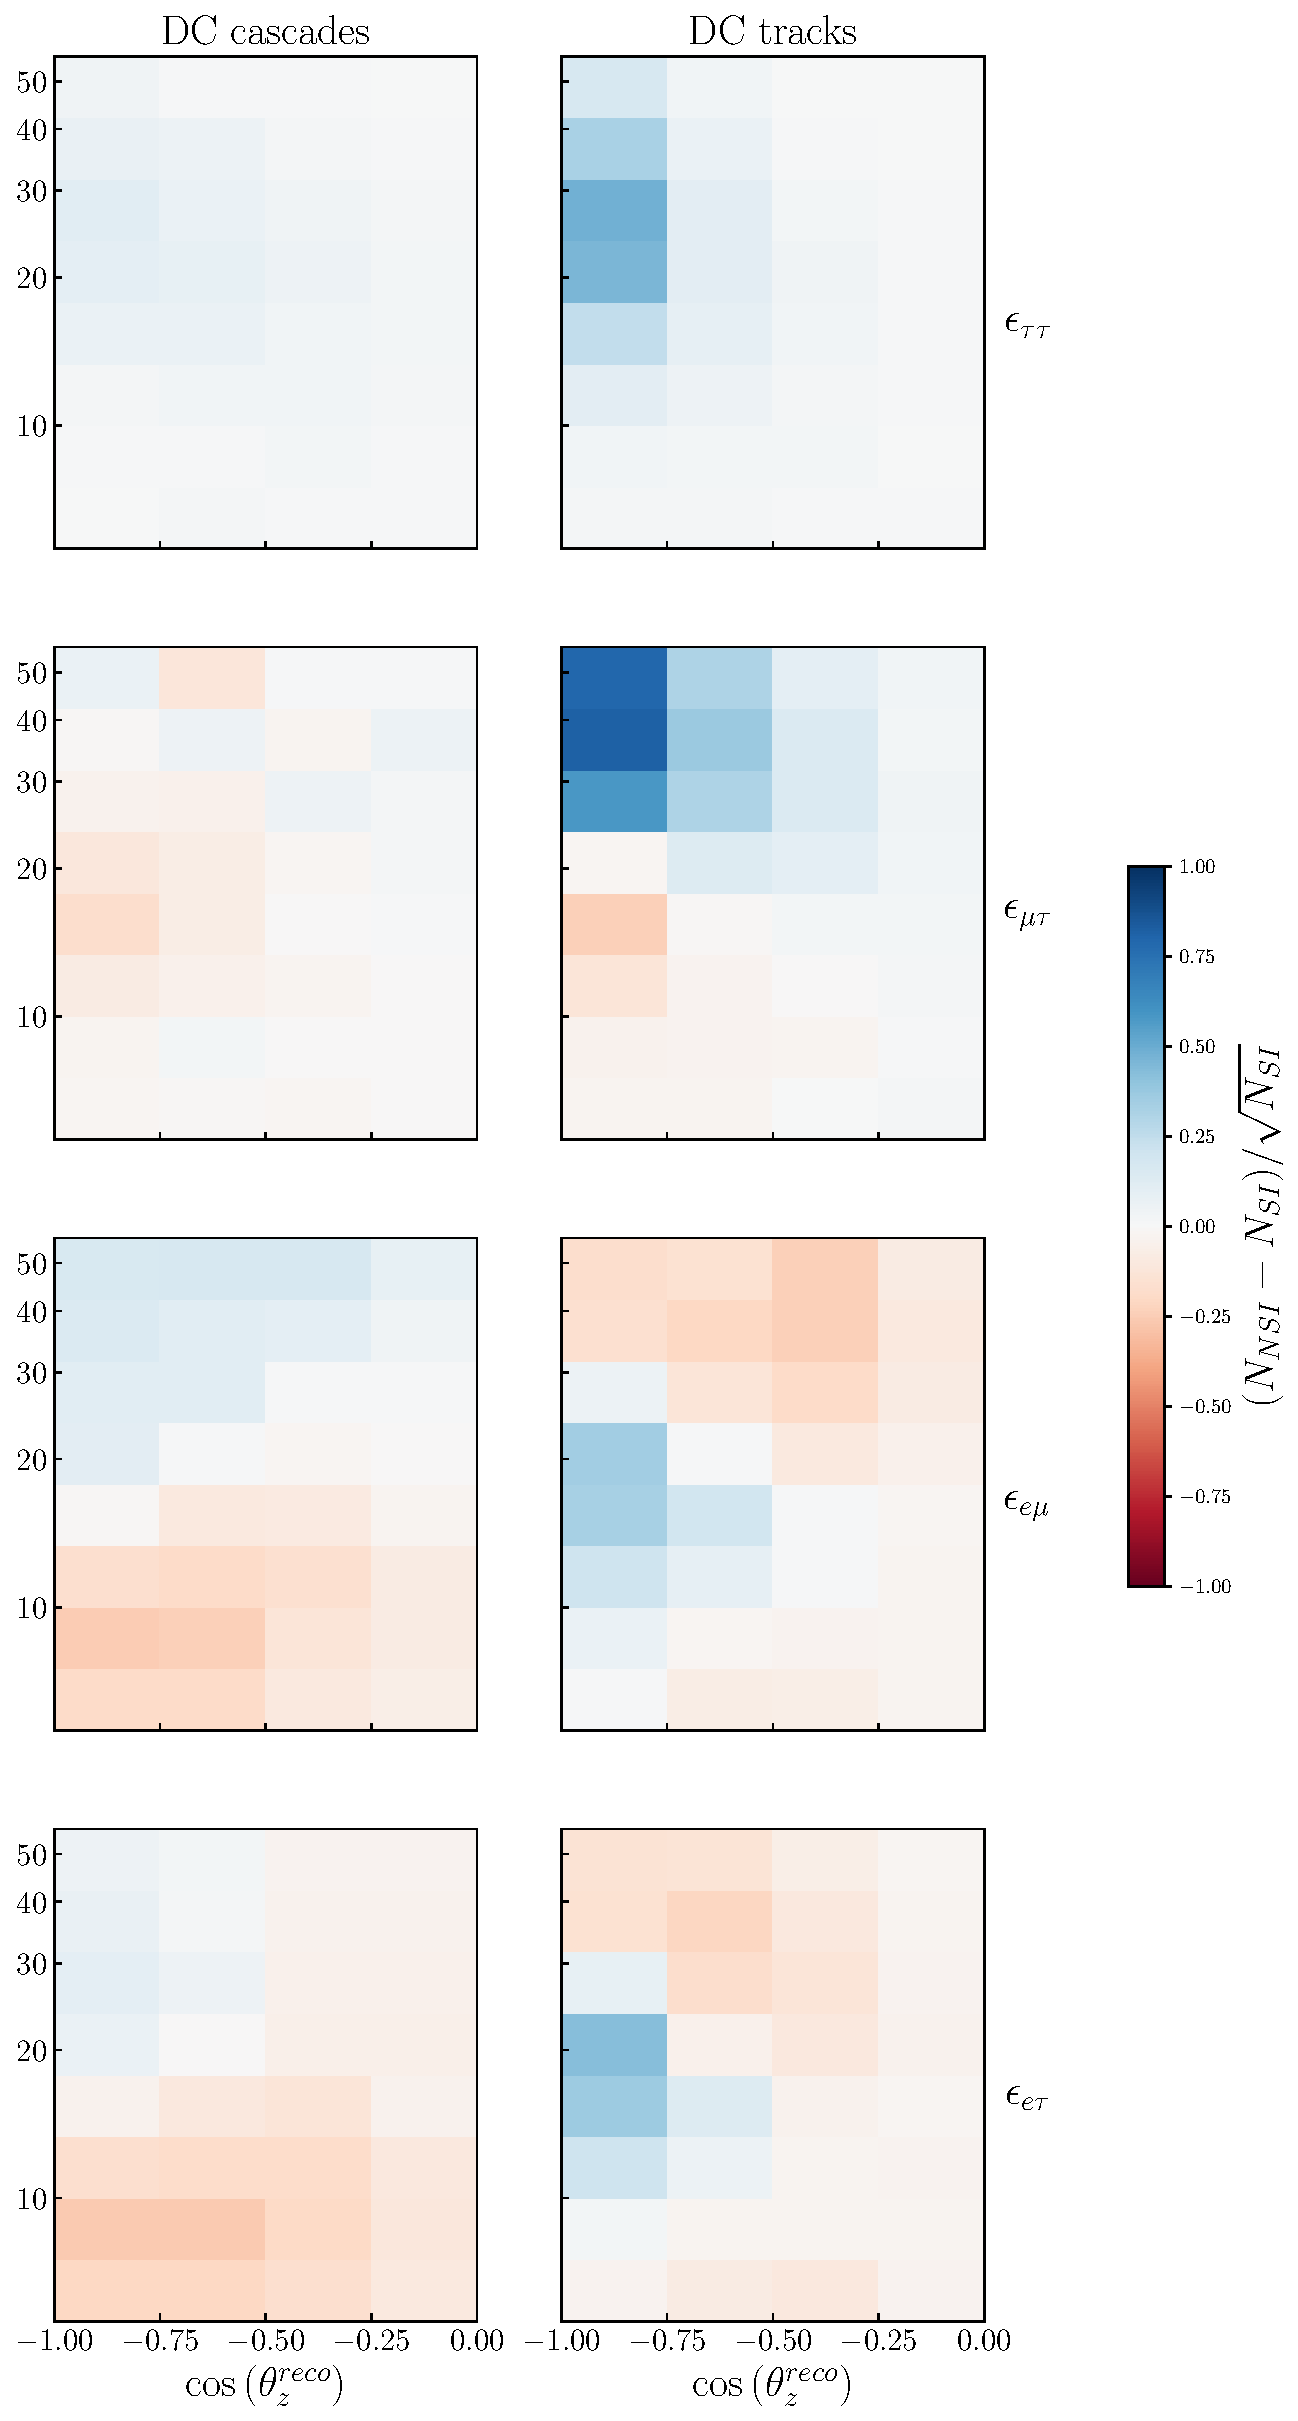
\includegraphics[width=1\linewidth]{figures/DC_event_pulls.pdf}
         \caption{DeepCore}\label{fig:DC_event_pulls}
      \end{subfigure}
    \end{center}
   \caption{Expected pulls of the form $(N_{NSI} - N_{SI})/\sqrt{N_{SI}}$ for PINGU and DeepCore after 3 years.}\label{fig:event_pulls} 
\end{figure}%TODO: redo these with same emt as flux_ratio? keep this, but align them better



%TODO: subsection about comparison between different papers. 

\begin{figure}
   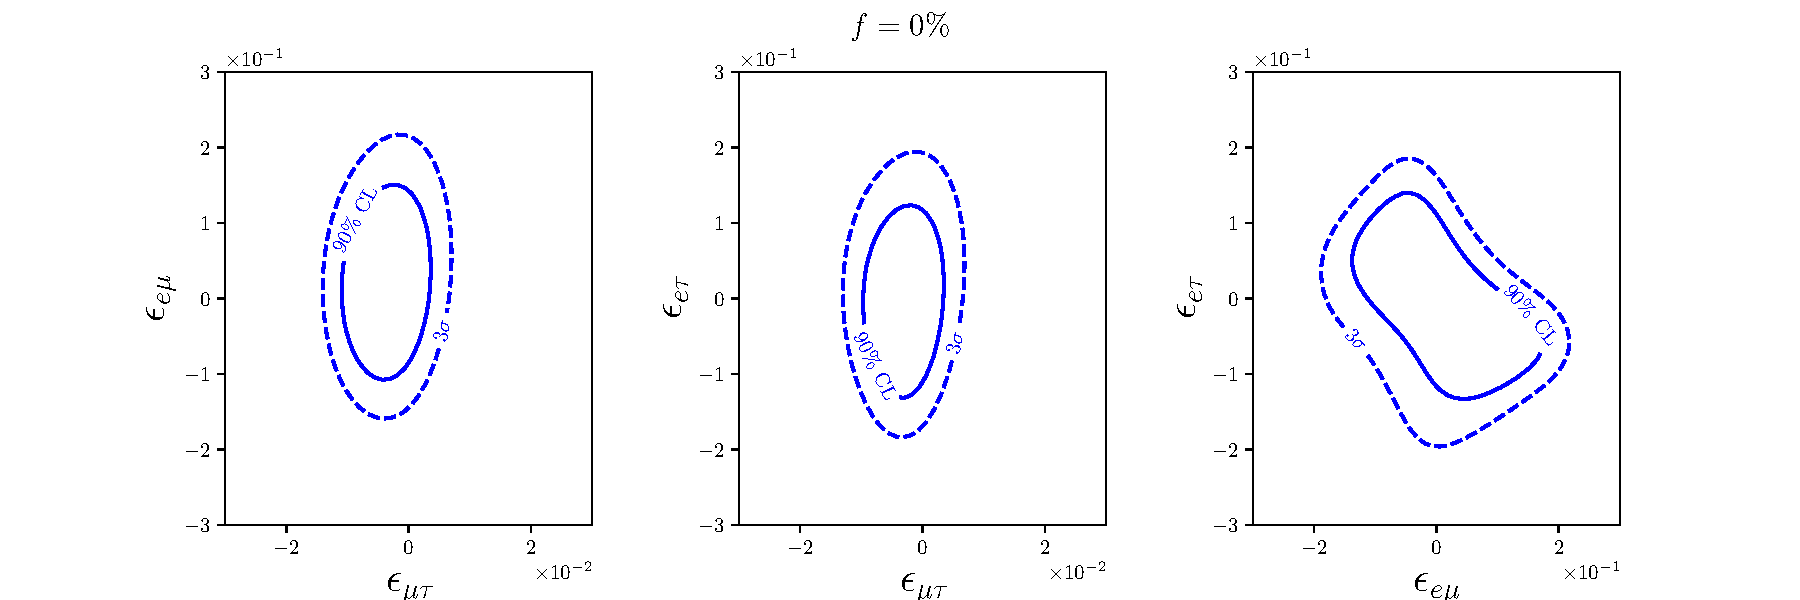
\includegraphics[width=0.9\textwidth]{figures/PINGU_2D_all_f0.pdf}
\end{figure}
\begin{figure}
   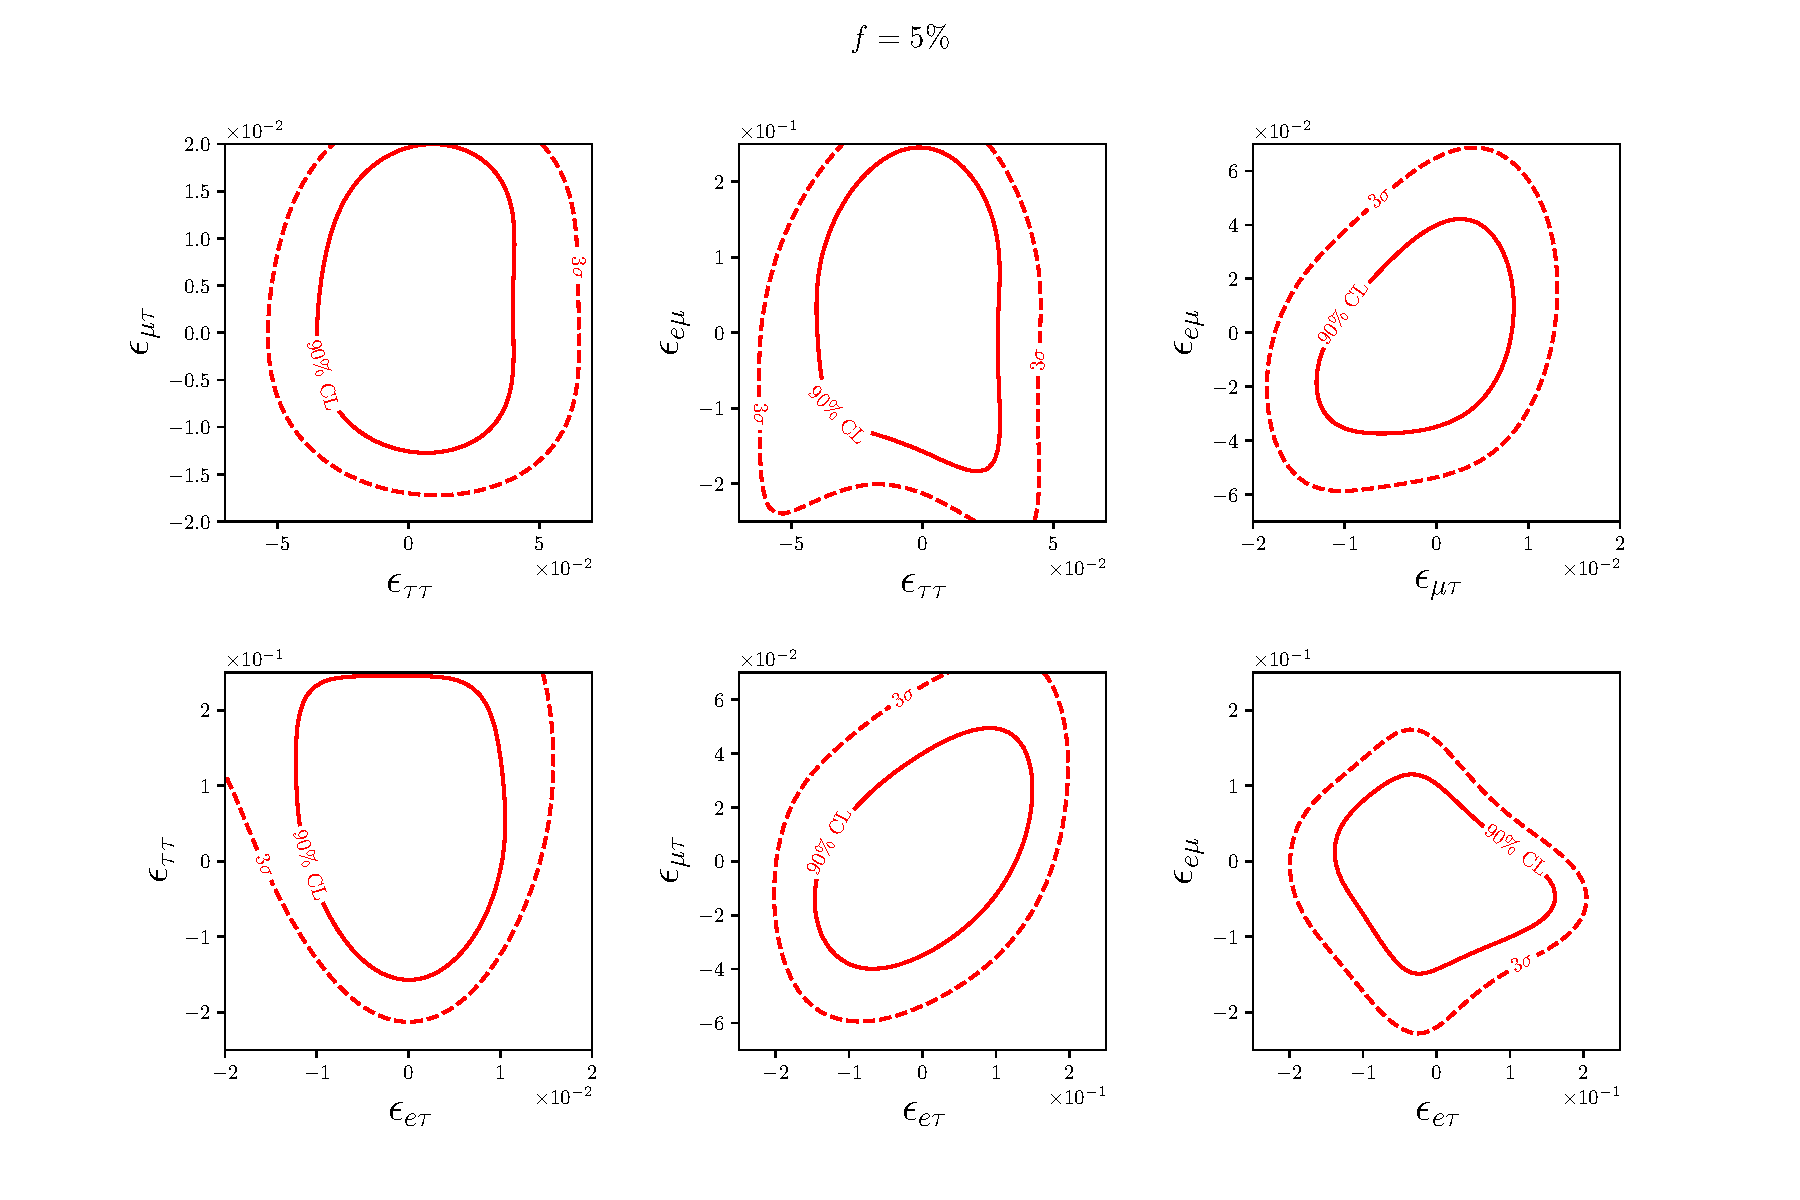
\includegraphics[width=0.9\textwidth]{figures/PINGU_2D_all_f5.pdf}
\end{figure}
\bibliographystyle{elsarticle-num}
\bibliography{article}

\newpage
\begin{tabular}{p{55mm}p{55mm}p{55mm}}
   DeepCore (2017)
      \begin{itemize}
         \item[$\checkmark$] Honda atmospheric fluxes
         \item[$\times$] Only look at tracks and $\emt$
         \vspace{1em}  
         \item[$\times$] DC Monte Carlo from an older dataset 
         \item[$\times$] 8 E bins from $\SI{6.3}{\electronvolt^2}$ to $\SI{56}{\electronvolt^2}$
         \item[$\times$] 8 z bins from -1 to 0 
         \item[$\times$] Use "Overall" and "relative $\ne$ to $\nm$" normalization
         \item[$\times$] Prior on spectral index
         \item[$\times$] No zenith angle normalization
         \item[$\checkmark$] No priors on $\dm, \theta_{23},\theta_{13}$
      \end{itemize} &
    Demidov (2020) DC analysis
      \begin{itemize}
         \item[$\checkmark$] Honda atmospheric fluxes
         \item[$\checkmark$] Looks at tracks + cascades for $\emt$ and $\ett$
         \item[$\checkmark$] Data and Monte Carlo from DC 2018
         \item[$\checkmark$] 8 E bins from $\SI{5.6}{\electronvolt^2}   $ to $\SI{56}{\electronvolt^2}$
         \item[$\checkmark$] 8 z bins from -1 to 1
         \item[$\times$] Use "Overall" and "relative $\ne$ to $\nm$" normalization
         \item[$\times$] Prior on spectral index
         \item[$\times$] No zenith angle normalization
         \item[$\checkmark$] No priors on $\dm, \theta_{23}$
         \item[$\checkmark$] Fixes $\Delta m^2_{21}, \theta_{12}, \theta_{13}$
         \item[$\times$] Uncertainty on hadron production in atmosphere
         \item[$\times$] Uncertainty on neutrino nucleon cross section 
      \end{itemize} &
    This DC+PINGU analysis
      \begin{itemize}
         \item[$\checkmark$] Honda atmospheric fluxes
         \item[$\checkmark$] Tracks and cascades for all flavors
         \vspace{1em} 
         \item[$\checkmark$] Reco $\to$ true mapping from Monte Carlo migration matrix
         \item[$\checkmark$] 8 E bins from $\SI{5.6}{\electronvolt^2}$ to $\SI{56}{\electronvolt^2}$
         \item[$\checkmark$] 8 zenith angle bins from -1 to 1
         \item[$\checkmark$] Flux normalization uncertainty of 25\%
         \item[$\checkmark$] Zenith angle uncertainty of 4\% 
         \item[$\checkmark$] No priors on oscillation parameters 
         \item[$\checkmark$] Marginalize $\dm$ and $\theta_{23}$. All other oscillation parameters are fixed.
      \end{itemize} 
\end{tabular}
\end{document}

% \end{document}

%% Bibliography 
% \cleardoublepage
% \phantomsection
% \addcontentsline{toc}{chapter}{Bibliography}
% \printbibliography
% \cleardoublepage
\bibliographystyle{elsarticle-num}
\bibliography{ref}
% \includepdf[pages={1-}]{papers/file1.pdf}
% \includepdf[pages={1-}]{papers/file2.pdf}

\end{document}